% \documentclass[report,a4paper,12pt,nomag]{jsbook} %環境が若干古い場合はこちら。但しabstractの挙動に注意。
\documentclass[a4paper,11pt,nomag]{jsreport} %2017年2月以降のTeX環境にある。

\usepackage[master]{thesis-sjis}

\begin{document}
%\layout
\題目={メタ学習に基づくInfrared Few-shot Open-set Recognitionを考慮した動物分類}
\学籍番号={K623009}           %%%  学籍番号
\氏名={岸 孝樹}             %%%  氏名
\提出{7}{1}{30}               %%%  提出年月日の順です.年は令和で.
\英文題目={Animal Classification Considering \\ Infrared Few-shot Open-set Recognition \\ Based on Meta-learning} %%%  英文のアブストラクトを書く場合.卒業論文ならコメントアウト.
\英文氏名={Koki Kishi}
\MakeTitle
\newpage
\begin{abstract}\hspace{0.5zw}
  % /01_draft/abstract/abstract_v2.tex

%英文のアブストラクトを書く場合.(200語程度)
Camera traps are crucial for cost-effective ecosystem monitoring.
In particular, there are high expectations for using infrared cameras to capture night images.
However, there are challenges with classifying infrared images, such as the lack of color information and insufficient training data.

This paper proposes the novel Infrared Few-shot Open-set Recognition (IFOR) framework for wildlife monitoring using camera traps.
The framework considers three key challenges: infrared image classification, limited training data, and unknown species detection.
We evaluated the effectiveness of meta-learning with different feature extractors (CNN and ViT) and transfer learning approaches within the IFOR framework.
Furthermore, to improve the multi-class classification accuracy for unknown animal species, 
k-means loss and Between-Class loss were introduced to minimize intra-class variance and maximize inter-class variance.
The experiments utilized data collected from different regions for training and evaluation and assessed the model's performance under domain shift conditions.
Experimental results showed that ViT with ImageNet pre-training and meta-learning was effective for IFOR, 
and the proposed loss functions effectively enhanced the classification accuracy of both known and unknown species.

The results of this research provide important insights for realizing effective wildlife monitoring systems under limited data conditions.
Moreover, they are expected to be a foundation for developing practical machine-learning models in ecological research.
\end{abstract}

% /01_draft/chapter1/chapter1_v3.tex

\chapter{序論}
\setcounter{page}{1}

生物多様性が生み出す生態的機能は,温室効果ガス,エネルギー,水などの物質・資源循環など,地球に不可欠な役割を多数持っており,人間社会の基盤となっている \cite{millennium-ecosystem2005,cardinale2011}.
生態的機能のうち,特に人間社会の便益につながるものを生態系サービスと呼ぶ.
しかしながら,昨今,人間による土地開発や気候変動によって,陸域生態系の劣化と生物多様性の損失は進行しており \cite{newbold2015,isbell2017},生態系サービスの享受が困難になっている.
したがって,生態系の劣化を低減し,生物多様性の損失を抑制することは,現代社会における根本的な社会課題であり,その解決が急務である.
これらの課題は持続可能な開発目標(SDG15: 陸の豊かさも守ろう)などの国際目標としても掲げられ,日本でも生物多様性国家戦略 \cite{biodiversity2023}をはじめとする様々な政策や企業の取り組みが開始されている.

これらの社会課題に対して,継続的な野生動物との共存を実現するため,生態系モニタリングが注目を集めている.
生態系モニタリングは,自然環境の空間的・時間的変化の把握に有効な方法であり,自然保護や環境保全に重要なデータを提供する.
モニタリング実施の効果として生態系に生じた異常の早期発見が可能であり,迅速な対策により生態系の回復期間の短縮やコスト削減へと繋がることが期待される.

費用対効果の高い生態系モニタリングを行う上で,カメラトラップの使用は極めて重要である \cite{jia2022}.
図 \ref{fig:cameratrap}にカメラトラップの例を示す.
% 
\begin{figure}[tbp]
  \centering
  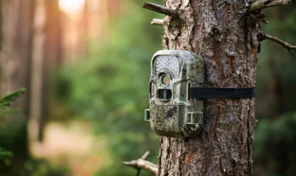
\includegraphics[width=0.5\linewidth, keepaspectratio]{image/cameratrap.png}
  \caption{カメラトラップの例}
  \label{fig:cameratrap}
\end{figure}
% 
カメラトラップは,赤外線センサなどを用いてカメラの前を通り過ぎる動物を感知し,自動的に撮影するため,動物にストレスを与えることなく,撮影者によるバイアスを排除したデータ収集が可能である\cite{newey2015,zhu2017}.
これらのカメラは,比較的低価格であり,限られた電力資源で効率的に動作するため,広範囲に長期間の撮影が可能である \cite{schneider2018, carl2020}.
また,赤外線カメラの使用により,夜間の撮影も可能である.
近年,カメラトラップによって膨大な画像や動画データが低コストで収集できるようになり,深層学習モデルを用いた野生動物の正確な検出と分類に期待が高まっている \cite{tan2022}.

野生動物画像の分類に関して,畳み込みニューラルネットワーク (Convolutional Neural Network,CNN) を用いた手法がいくつか提案されている \cite{manna2023,mohanty2022, agarwal2023, neeli2023}.
しかし,自然環境下における野生動物に対する分類タスク特有の課題として,特定地域における十分な量の学習用画像の収集コストが高いことや \cite{schneider2020},赤外線カメラによって撮影された画像は色情報が欠落していること \cite{kishimoto2023}などが挙げられる.
図 \ref{fig:camera}に撮影方法(カメラ)の違いによる物体の写り方の違いを示す.
既存の動物分類手法のほとんどは図 \ref{fig:color_deer}のような可視光画像に焦点を当てており,図\ref{fig:infrared_deer}のような赤外線画像に対して取り組んだ研究は少ない.
また,赤外線画像と可視光画像では物体の写り方が大きく異なるため,既存の可視光画像に対する手法を赤外線画像に対して適用した場合,精度が大きく低下する.

\begin{figure}[tbp]
  \centering
  \begin{subfigure}[b]{0.45\linewidth}
    \centering
    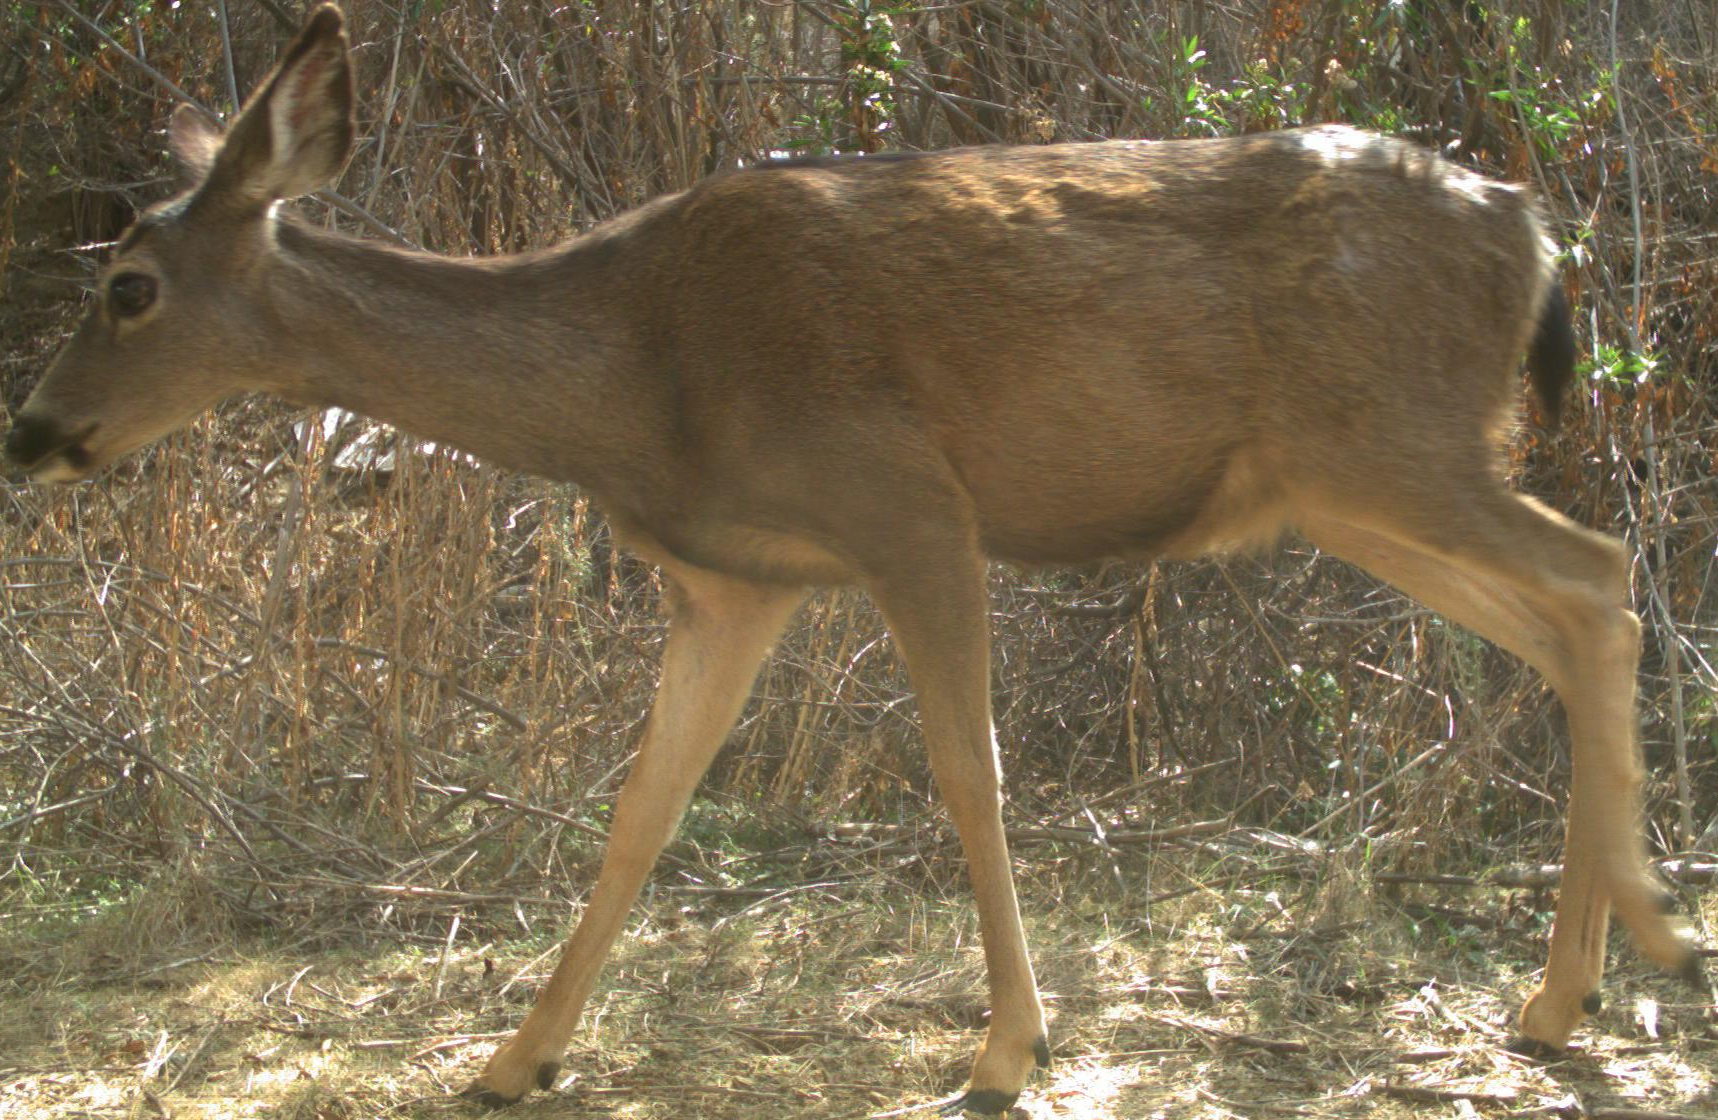
\includegraphics[height=0.7\linewidth, keepaspectratio]{image/cct_color_deer.png}
    \caption{可視光画像}
    \label{fig:color_deer}
  \end{subfigure}
  \hfill
  \begin{subfigure}[b]{0.45\linewidth}
    \centering
    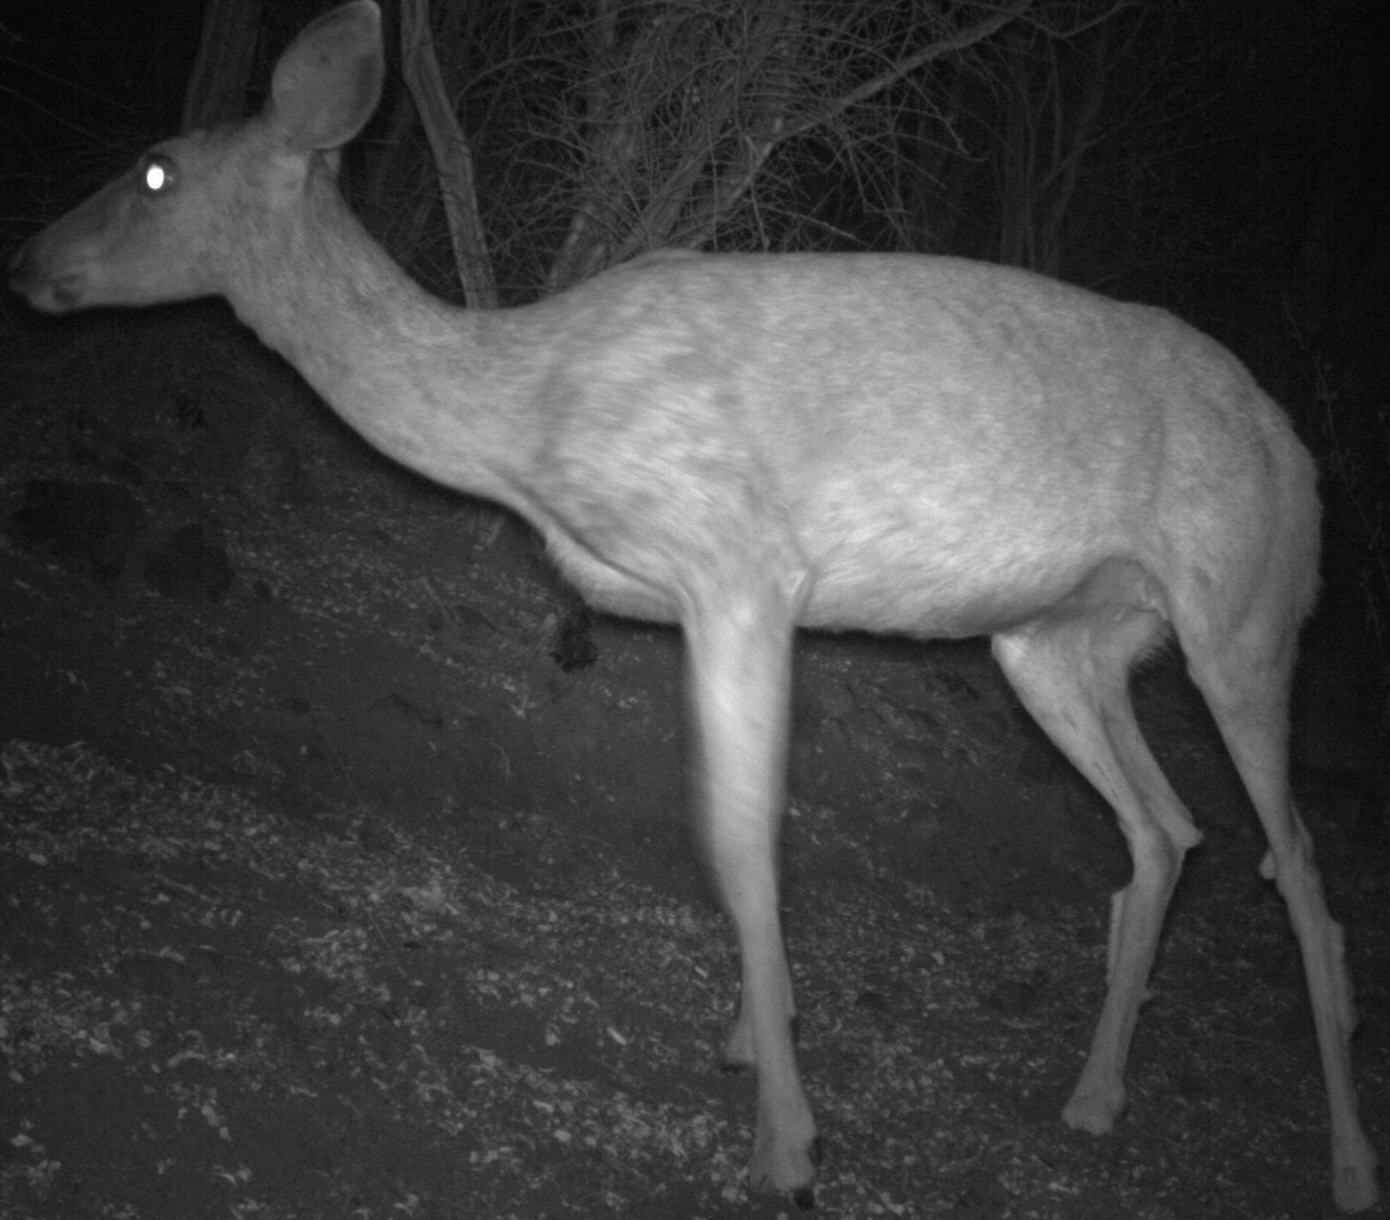
\includegraphics[height=0.7\linewidth, keepaspectratio]{image/cct_infrared_deer.png}
    \caption{赤外線画像}
    \label{fig:infrared_deer}
  \end{subfigure}
  \caption{撮影方法(カメラ)の違いによる物体の写り方}
  \label{fig:camera}
\end{figure}

このような課題を解決するため,少数の赤外線画像を深層学習モデルの学習に用いた動物分類に関する研究が行われている \cite{kishimoto2023}.
しかし,既存研究では,評価時に分類対象となる動物種は全て学習済みであると仮定しているが,実運用において,深層学習モデルを特定の地域に適用する際,モデルが対象地域に生息する全ての動物種を学習しているとは限らない.
このような状況において,未学習の動物種は学習済みの動物種に強制的に誤分類され,モデルの性能は著しく低下することが知られており,
この問題はオープンセット問題 (Open-Set Problem) \cite{osr} と呼ばれる.
このオープンセット問題に対処するため,学習済みクラスの分類を行いつつ,
未学習クラスを検出するオープンセット認識 (Open-Set Recognition,OSR) 手法が提案されている \cite{sun2020, sagar2022}.

さらに近年では,少数データでもオープンセット認識を可能にする Few-Shot Open-Set Recognition (FSOSR) \cite{peeler} が注目を集めている.
代表的なFSOSR手法として,少数データ学習 (Few-Shot Learning,FSL) 分野で有効な手法とされているメタ学習をOSRに拡張することによりFSLとOSRを同時に実現したPEELER \cite{peeler}や,
変換の一貫性に基づき未学習クラスを検出することによって,擬似的な未学習クラスサンプルを必要としないSnaTCHer \cite{snatcher}が挙げられる.
しかし,これらの手法は可視光画像を対象としており,赤外線画像に対する性能評価が行われていない.
また,FSOSRでは未学習クラスを単一種として扱っているが,新しい動物種に対するアノテーションや追加学習に要するコストを考慮すると,実用的には未学習クラスも複数種に分類できることが望ましい.

本論文では,夜間の野生動物モニタリングの実現を目的とした,より実用的な問題設定である「Infrared Few-shot Open-set Recognition (IFOR)」を提案する.
IFORでは少量の赤外線画像データのみを用いて,特定地域に生息するモデルに学習済みの動物種を正確に分類し,かつ,未学習の動物種の検出を可能にすることを目指す.
加えて,IFORではドメインシフトに対する頑健性の評価も必要である.
ドメインシフトとは,学習データと評価データが異なる地域で収集された場合に生じる課題であり,背景や撮影環境の違い,同じ動物種の地域差による外見の違いなどによってモデルの性能が低下する現象を指す.
ドメインシフトを考慮することにより,地理的条件に依存せず,様々な場所に適用可能な汎用性の高いシステムの実現が期待される.

本論文では,IFORの実現に向けて,赤外線画像に有効な既存手法の特定に加え,既存のFSOSR手法の1つであるメタ学習フレームワークがIFORに対して効果的であるか検証を行う.
まず,赤外線画像に有効な特徴抽出器を特定するため,テクスチャ特徴に焦点を当てているCNNや,
形状特徴 \cite{feature}を重視することで知られている Vision Transformer (ViT) \cite{vit}などの代表的な特徴抽出器の有効性を赤外線画像に対して評価する.
次に,IFORフレームワーク内のFSLタスクに有効なアプローチの1つである転移学習について検証する.
転移学習では,事前学習のタスクと本番環境でのタスクの類似度が重要だと考えられている.
そこで,一般的なImageNetデータセットを用いた事前学習と並行して,事前学習に色情報を持たないフラクタル画像を用いるFormula-Driven Supervised Learning (FDSL) \cite{fdsl}の有効性を探る.
最後に,赤外線画像を分類する際,小規模データセットから汎用的な特徴抽出を行うための学習戦略であるメタ学習のIFORにおける有効性を,ドメインシフトの条件下で評価する.
特に,IFORにおいては学習済みクラスの正確な画像分類と未学習クラスの検出が不可欠であるため,メタ学習による有効性を従来の学習方法であるミニバッチ学習と比較する.

さらに,IFORを発展させ,未学習クラスに対する多クラス分類の精度向上にも取り組む.
特徴空間上で各学習済みクラスの分布がコンパクトに表現されることにより,未学習データに対しても多クラス分類が容易になると仮定し,
クラスタリングに基づく損失関数を用いてクラス内分散の最小化・クラス間分散の最大化を図る.
クラス内分散の最小化では,異常検知タスクで用いられているk-means損失 \cite{k-means} を導入する.
クラス間分散の最大化では,k-meansクラスタリングによって得られる各クラスタ中心を利用した損失関数であるBetween-Class損失(BC損失)を提案する.

以下,第2章では深層学習を用いた動物分類に関する既存研究について述べる.
第3章では夜間の野生動物モニタリングの実現に向けてより実用的な問題設定を提案し,様々な手法の有用性について述べる.
第4章では評価実験を行い,その結果及び考察を多面的な方向から述べる.
最後に第5章では結論を述べる.
% /01_draft/chapter1/chapter1_v3.tex

\chapter{深層学習を用いた動物分類に関する既存研究}

\section{赤外線画像に対する動物分類に関する既存研究}

気候変動や人口増加が生態系に与える影響を把握し,野生動物と人間の持続可能な共存を実現することは重要な課題である.
この課題を解決するため,生態系モニタリングの重要性が世界的に高まっている \cite{zwerts2021, bandaru2024}.
生態系モニタリングの手法として,監視カメラなどを用いた観測が広く採用されており,特定地域における動物種の個体数推定だけでなく,固有の環境に対する各動物種の生態観察や研究が行われている \cite{trolliet2014}.
特に,カメラトラップは,観察者による直接的な介入を最小限に抑えることが可能であり,観察者の存在が個体の行動に与える影響を軽減することができるため,
野生動物の監視ツールとして広く活用されている \cite{本郷2018, abood2023}.
カメラトラップは,赤外線センサなどを用いた自動撮影により人的労力を削減することができ,近年のデジタルカメラの高性能化に伴い長期間にわたる連続的なモニタリングが可能である.
一方で,カメラトラップを使用した生態系モニタリングでは,複数箇所にカメラトラップを設置するため膨大な画像枚数を取得することも多く \cite{kays2020, si2014},
記録された画像・動画中に対する人手による動物の有無や種の推定は多大なアノテーションコストを要する \cite{thangaraj2023}.
加えて,種の分類には専門的な知識が必要であることも作業員確保によるコスト面での課題である.
さらに,技術革新は今後も進むと予想されるのに対し,アノテーションコストを著しく下げることは困難であるため,このギャップは今後一層拡大していくと予想される \cite{安藤2019}.
したがって,これらの課題を解決するため,カメラトラップによって撮影された画像・動画中から自動で動物を検出・識別する手法の実現が望まれている.

近年では,画像処理技術と機械学習を用いた野生動物の自動識別手法が研究されている \cite{manna2023, mohanty2022}.
国際的な画像認識アルゴリズム性能コンペティションとして知られるImageNet Large Scale Visual Recognition Challenge (ILSVRC) の2012年大会において,
AlexNet \cite{alexnet}が画期的な成功を収めて以降,画像処理分野の様々なタスクにおいてCNNに基づく手法が盛んに研究されている \cite{mohanty2016, sue2020}.
また,その多くのタスクでCNNは高い性能を実現しており,カメラトラップによる動物識別に関する研究においてもCNNを用いた手法がいくつか提案されている \cite{agarwal2023, neeli2023, abood2023, thangaraj2023}.
Tanら \cite{tan2022}は,2014年から2020年にかけて撮影された約25,000枚の自作データセットを用いて,YOLO-V5 \cite{yolov5},FCOS (Fully Convolutional One-Stage Object Detection) \cite{fcos},
Cascade R-CNN \cite{cascade}の3つの検出ネットワークでの比較検証,及び映像に適用した動物認識の性能を評価している.
Tabakら \cite{tabak2019}は,全米5箇所で撮影された約300万枚のカメラトラップ画像を用いて,独自のCNNにより動物の画像分類を行っている.

しかしながら,上記のような既存研究の分類モデルを学習するために用いられた大規模なデータセットは,多くの撮影場所や数年間に及ぶ長期間の撮影によって蓄積された画像で構成されている.
そのため,これらの既存研究は個人的な利用での撮影や狭い範囲の地域での撮影など,十分な画像データを収集できない状況には適しておらず,実用面での課題が残る.
また,夜間に行動する動物の撮影には赤外線カメラを用いることが有効であるが,赤外線カメラで撮影された画像は色情報を含まないなど,可視光カメラで撮影された画像とは映り方が異なる.
したがって,真に実用的な生態系モニタリングシステムの実現に向けて,赤外線カメラによって撮影された少数の学習用データから,効率的に学習可能な深層学習モデルの開発が急務である.

このような既存研究の課題解決に向けた研究として,少数の赤外線画像を用いた動物分類が検討されている.
Kishiら \cite{kishimoto2023}は,米国南西部の140箇所で撮影された画像3,000枚を用いて,CNNによる少数の赤外線画像を用いた動物分類を行っている.
この先行研究では,少数データを用いた効率的な深層学習モデルの学習を目的とするFSLの分野において有効な手法である転移学習とデータ拡張の赤外線画像に対する有効性が検証された.
まず,転移学習は,事前に大量のデータを用いて学習したモデルを新しいタスクに適用する手法である.
この先行研究では,画像認識タスクで一般的に用いられるImageNetデータセット,ImageNetデータセットを擬似赤外線化した画像,
さらに数式から生成されたフラクタル画像による転移学習の有効性が検証された.
一方,データ拡張については,一般的な幾何学変換や色変換などの画像変換に加え,画像の一部をマスクし隠すことでモデルの汎化性能を向上させるRandom Erasingや,
複数の画像処理を組み合わせることで新しい画像を生成しモデルの頑健性を向上させるAugmixなどの有効性が検証された.
実験の結果,転移学習では疑似赤外線画像,フラクタル画像,ImageNetの順に効果が高いことが示され,データ拡張についてはAugMixが特に有効であることが明らかになった.

Kishiらの研究では,新規地域に対する深層学習モデルの適用開始時の状況を想定しており,学習に使用する画像は1クラスあたり50枚としている.
しかし,実運用を想定すると1クラスあたり50枚程度の画像収集すら困難な場合も考えられる.
また,評価実験における評価用データセットでは学習用データセットと同じ動物種のみが使用されており,モデルの適用地域に生息する全ての動物種がモデルに登録されている閉集合が仮定されている.
しかし,モデルの実運用開始時において,対象地域に生息する全ての動物種のデータを網羅的に収集することは現実的ではない.
従来の分類モデルでは,学習データに含まれていないモデルに未登録の動物を正しく識別できず,登録済みのクラスに強制的に分類されてしまうオープンセット問題が存在する.
図 \ref{fig:non_osr}は,従来の分類モデルが未登録の動物を識別できない例を示している.
% 
\begin{figure}[tbp]
  \centering
  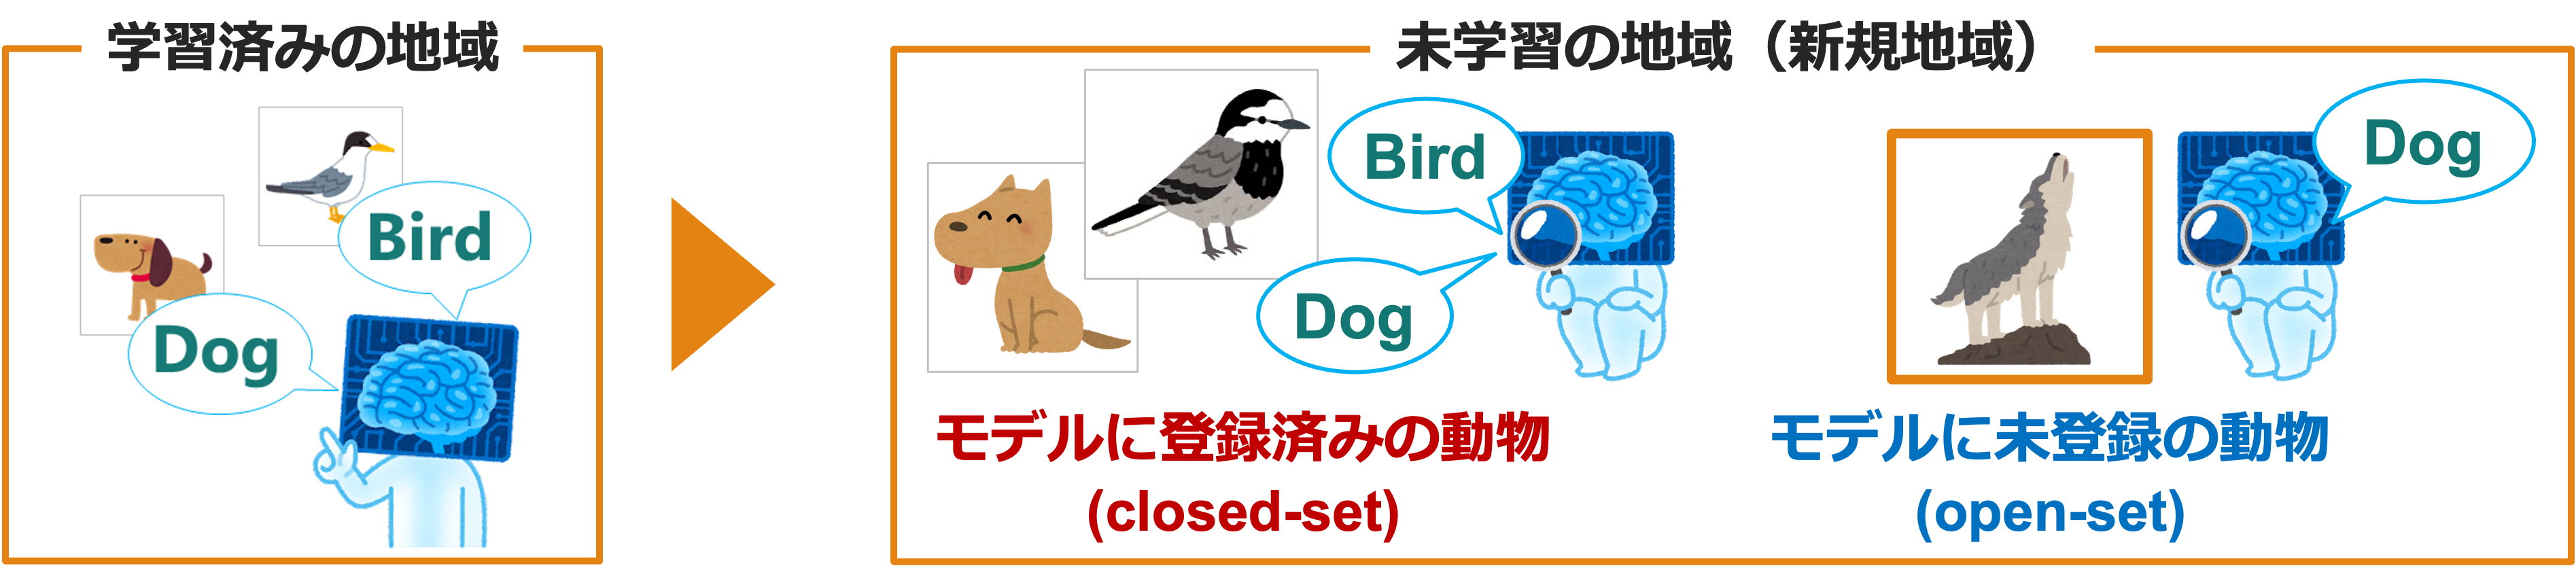
\includegraphics[width=\linewidth, keepaspectratio]{image/non_osr.png}
  \caption{従来の分類モデルによるオープンセット問題の例}
  \label{fig:non_osr}
\end{figure}
% 
図 \ref{fig:non_osr} に示される通り,犬と鳥のみを学習したモデルを新規地域に適用した場合,モデルに登録済みの犬や鳥は分類できるが,未登録の動物であるオオカミは登録済みの動物種に強制的に分類されてしまう.
このような誤分類はモデルの精度低下へと繋がるため,未登録の動物種を適切に検出できるOSRモデルの開発が急務となっている.
なお,本論文では,モデルに登録されているクラスセットをクローズドセット (closed-set),モデルに未登録のクラスセットをオープンセット (open-set)と呼ぶ.


\section{Few-Shot Open-Set Recognitionに関する既存研究}

昨今の第3次AIブームにおける機械学習システムの高い性能や実用的な成果は,主にクローズドセットタスクにおいて達成されてきた.
これらのシステムでは,学習用データセットと評価用データセットに同一のクラスが含まれることを前提としており,システムの評価は学習時に登録されたオブジェクトクラスのみを対象として実施される.
しかしながら,より実用的なシステムの実現を目指す場合,現実的な問題設定としてオープンセット問題への対応が不可欠である \cite{geng2021survey}.
機械学習ベースのシステムの利用が進むにつれ,幅広いアプリケーションにおいて高い頑健性を備えた手法が要求されており,OSR技術に注目が集まっている \cite{sun2023survey}.
OSRは,学習時に想定していないクラスのデータが入力された場合でも,システムを頑健に機能させるためのアプローチの1つとして位置付けられている.
図 \ref{fig:osr}にOSRにおける未登録データの検出プロセスの一例を示す.
% 
\begin{figure}[tbp]
  \centering
  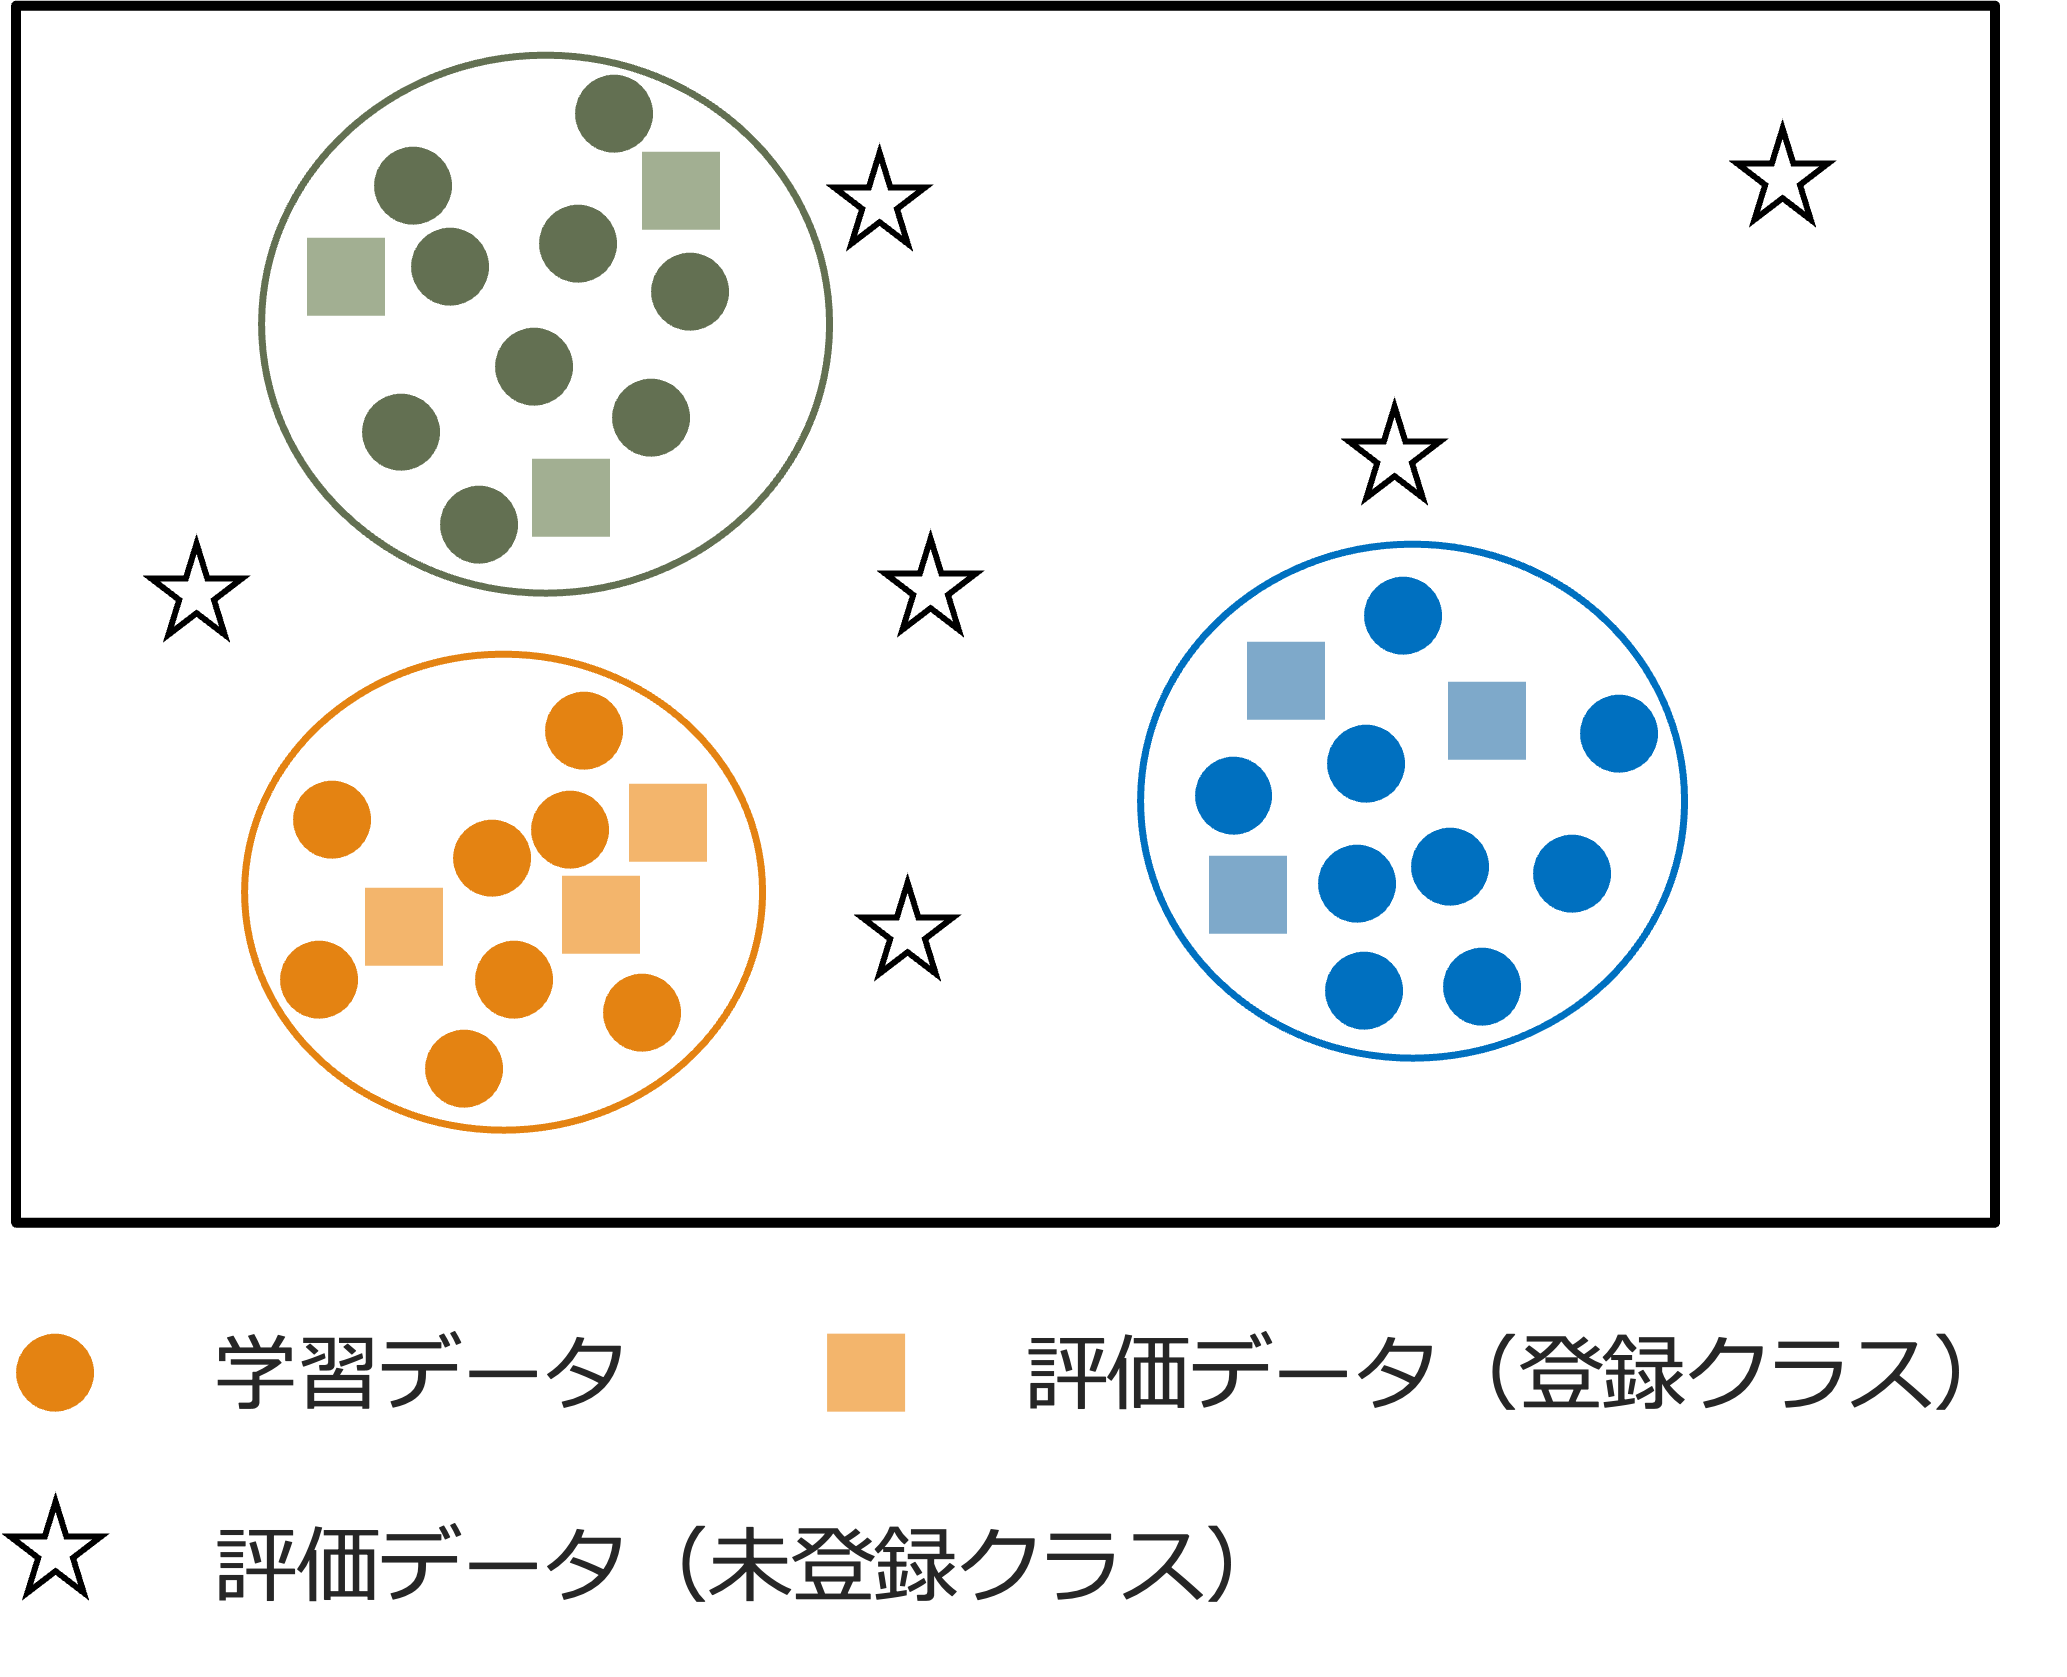
\includegraphics[width=0.6\linewidth, keepaspectratio]{image/osr.png}
  \caption{OSRにおける未登録データの検出プロセスの一例}
  \label{fig:osr}
\end{figure}
% 
既存の分類モデルでは未登録データを登録クラスに分類してしまう課題があったが,分類対象の画像の特徴量と登録クラスの類似度が特定の閾値を下回る場合に未登録クラスとして検出することで,
この課題を解決することが可能となった.

実世界における動的な環境下での認識・分類タスクに対して,より実用的なモデルを構築するためには未登録クラスへの対応が不可欠である.
% これを考慮しない場合,システムの不適切な開発につながり,その有用性が著しく制限されることとなる.
しかし,学習時に想定されていないクラスは無数に存在する可能性があり,それら全てを事前に予測して学習データに含めることは現実的ではない \cite{mahdavi2021survey}.
特に,深層学習モデルはデータ駆動型のアプローチのため,適切な帰納バイアスを獲得するために大量の学習データを必要とする.
同様に,既存のOSR手法においても大量の学習データの利用を前提としており,その適用範囲は局所的な場面に限定されている \cite{wang2023}.

この課題に対し,近年ではFew-Shot Open-Set Recognition (FSOSR) という新たな研究分野が注目を集めている \cite{peeler, che2023}.
FSOSRは,少数の画像データからの効率的な学習による正確な分類を行うことと,学習データに存在しないデータを未登録クラスとして検出・拒絶できるモデルの構築を目的とした研究分野である.

Jeongら \cite{snatcher}は,変換一貫性 (transformation consistency) という概念に基づき,未登録クラスを検出するSnaTCHerを提案した.
これは,類似した入力データは特徴空間での変換後も近い位置関係を保つという性質を利用している.
未登録クラスの入力データは,登録クラスとは異なる特徴空間を形成する傾向があるため,変換後の特徴量は登録クラスのプロトタイプから大きく離れることが期待される.
プロトタイプとは,登録クラスを代表する特徴ベクトルのことであり,登録クラスから得られた特徴量の平均値を求めることによって生成される.
この手法の最大の利点は,疑似的な未登録クラスサンプルを必要としない点である.
OSRなどにおける従来手法が未登録クラスの分布を直接推定するのに対し,SnaTCHerは特徴量の相対的な変換問題として扱うことで,より効率的な学習を実現した.
また,様々な特徴量変換手法との組み合わせ実験により,分類性能を低下させることなく,未登録クラスサンプルの検出性能を向上させることが確認された.

一方で,Huangら \cite{tane}は,閾値の設定に依存しない新しい手法としてTask-Adaptive Negative Envision (TANE) を提案した.
TANEは,登録クラスのプロトタイプから負例のプロトタイプを生成し,これを用いてタスクに応じた動的な拒絶境界を学習する.
具体的に,登録クラスの代表点に注意機構を適用して負例のプロトタイプを生成し,入力データとの類似度が計算される.
もし全ての登録クラスに対する予測スコアが負例プロトタイプに対するスコアよりも低い場合,その入力データは未登録クラスとして拒絶される.

本論文では,限られたデータに対する赤外線動物分類の実現に向けて新しい問題設定を提案するとともに,今後の赤外線動物分類タスクの発展に向けて様々な手法の有効性を検証する.
% /01_draft/chapter3/chapter3_v3.tex

\chapter{メタ学習に基づくInfrared Few-shot Open-set Recognitionを考慮した動物分類}

\section{Infrared Few-shot Open-set Recognition (IFOR)}
\label{sec:ifor}

夜間に活動する動物を撮影するためには赤外線カメラを用いる必要があり,その結果として得られる画像は赤外線画像に限定される.
しかし,既存の分類モデルのほとんどは可視光画像を対象としており,色情報を持たない赤外線画像への適用可能性については未だに検証の余地が残されている.
本論文では,夜間における生態系モニタリングの実現に向けて,より実用的なモデルの構築支援を目的とし,
少数の赤外線画像を用いた動物分類と未登録の動物識別という新たな問題設定Infrared Few-shot Open-set Recognitionを提案する.
IFORでは,特定の地域に生息する野生動物の画像を大量に収集することが困難である現状を考慮し,モデルの学習に使用できるデータが限られている環境下でのシステムの運用を想定している.
そのため本論文では,より実用的な夜間の生態系モニタリングに向けて,
各クラス当たり1枚から30枚程度の少数画像を学習に用いた分類を行う.

また,収集されるデータが限られているという制約により,モデルの学習データは特定の地域に生息する動物を網羅的に含んでいない可能性が高い.
したがって,実運用の際には学習データに含まれない動物が出現する可能性が考えられる.
このような状況下では,モデルが未登録の動物を認識できずに登録済みのクラスに誤って分類してしまうため,未登録の動物種を正しく検出するシステムの実現が望まれている.

加えて,IFORでは,モデルの性能評価において,学習に用いたデータセットとは異なる地域で収集されたデータセットを評価時に使用する.
これにより,地域間における環境や動物種の差異など,新規地域に対するモデルの適応能力を評価することが可能となる.
このように,学習用データセットと評価用データセットのデータ分布が異なる状況はドメインシフトと呼ばれる.
IFORでは,この地域間のドメインシフトを意図的に導入することにより,モデルの頑健性と汎用性を定量的に評価し,
より広範な地域に対して適用可能なモデルの開発を推進する.

\section{IFORに対して有効な一手法の提案}
\label{sec:detection_approach}

本節では \ref{sec:ifor}節で提案したIFORフレームワークに対する効果的な手法について論じる.
提案手法は,IFORを構成する「赤外線画像」,「少数データ学習」,「未登録クラスの検出」という三つの要素に着目し,
各要素に対して効果的なアプローチを組み合わせることで,より高度な動物分類の実現を目指すものである.
第一に,赤外線画像における特徴抽出に関して,CNNとViT \cite{vit}という異なる特性を持つ二種類の特徴抽出器の有効性を検証する.
第二に,少数データの問題に対しては,ImageNetやFDSLなどの大規模データセットを用いた転移学習により,モデルの汎化性能の向上を図る.
第三に,未登録データへの対応として,メタ学習アルゴリズムを導入し,少数データにおける分類精度と未登録クラスの検出能力の向上を実現する.

\subsection{特徴抽出器}

画像処理分野において,深層学習技術の登場以降,様々な分野においてCNNを用いた手法が盛んに研究されている.
これらの手法は様々なタスクにおいて高い精度を実現しており,従来のハンドクラフト特徴量に基づいた識別手法によるアプローチから,
大規模な画像データセットを用いて学習されたCNNの使用へと顕著なパラダイムシフトをもたらした.

CNNの一種であるResidual Networks (ResNet) \cite{resnet}は深い畳み込みニューラルネットワークを効率的に訓練するために開発された深層学習モデルである.
本研究では,畳み込みニューラルネットワークの層が18層であるResNet18を使用する.
ResNet18は層が比較的浅く,小規模なデータセットにおいて有効性が示されているため,本研究の特徴抽出器として採用する.

一方,近年CNNに対する新たなアプローチとして,畳み込みを使用しないViTが注目を集めている.
ViTは,自然言語処理タスクで成功を収めたTransformerを画像処理タスクに応用したものであり,画像認識の多くの分野においてCNNよりも高い性能を発揮している.
ただし,ViTが最大限のモデルパフォーマンスを発揮するためには大規模なデータセットで学習を行う必要があり,
転移学習を行わない場合にはCNNと比較して性能が低下することが知られている \cite{vit}.

先行研究において,CNNはテクスチャ特徴の抽出に優れているのに対し,ViTは形状特徴の抽出に重点を置いていることが示されている \cite{feature}.
本研究で対象とする赤外線画像は色情報を欠いているため,分類時には形状特徴がより重要な手がかりとなる.このことから,形状特徴の抽出に優れたViTは赤外線画像の分類により適していると考えられる.
そこで,異なる特性を持つ2つの特徴抽出器としてResNet18及びViTを用いて,赤外線画像に対する有効性を比較検証する.

さらに本論文では,赤外線画像に対して基盤モデルを用いた意味的な特徴抽出にも取り組む.
上述したようなCNNやViTは画像のみを用いた学習を行うため,獲得できる表現能力に制限があった.
しかし近年の研究では,テキストと画像のペアを用いた学習によって,より効果的な画像表現の学習が可能であることが示された.
特に,Alecらはウェブから得た膨大なテキストと画像のペアを学習することにより,様々な下流タスクに転用可能な基盤モデル Contrastive Language-Image Pre-training (CLIP) を提案した \cite{clip}.
図 \ref{fig:clip-a}にCLIPの事前学習の概要を示す.
% 
\begin{figure}[tbp]
  \centering
  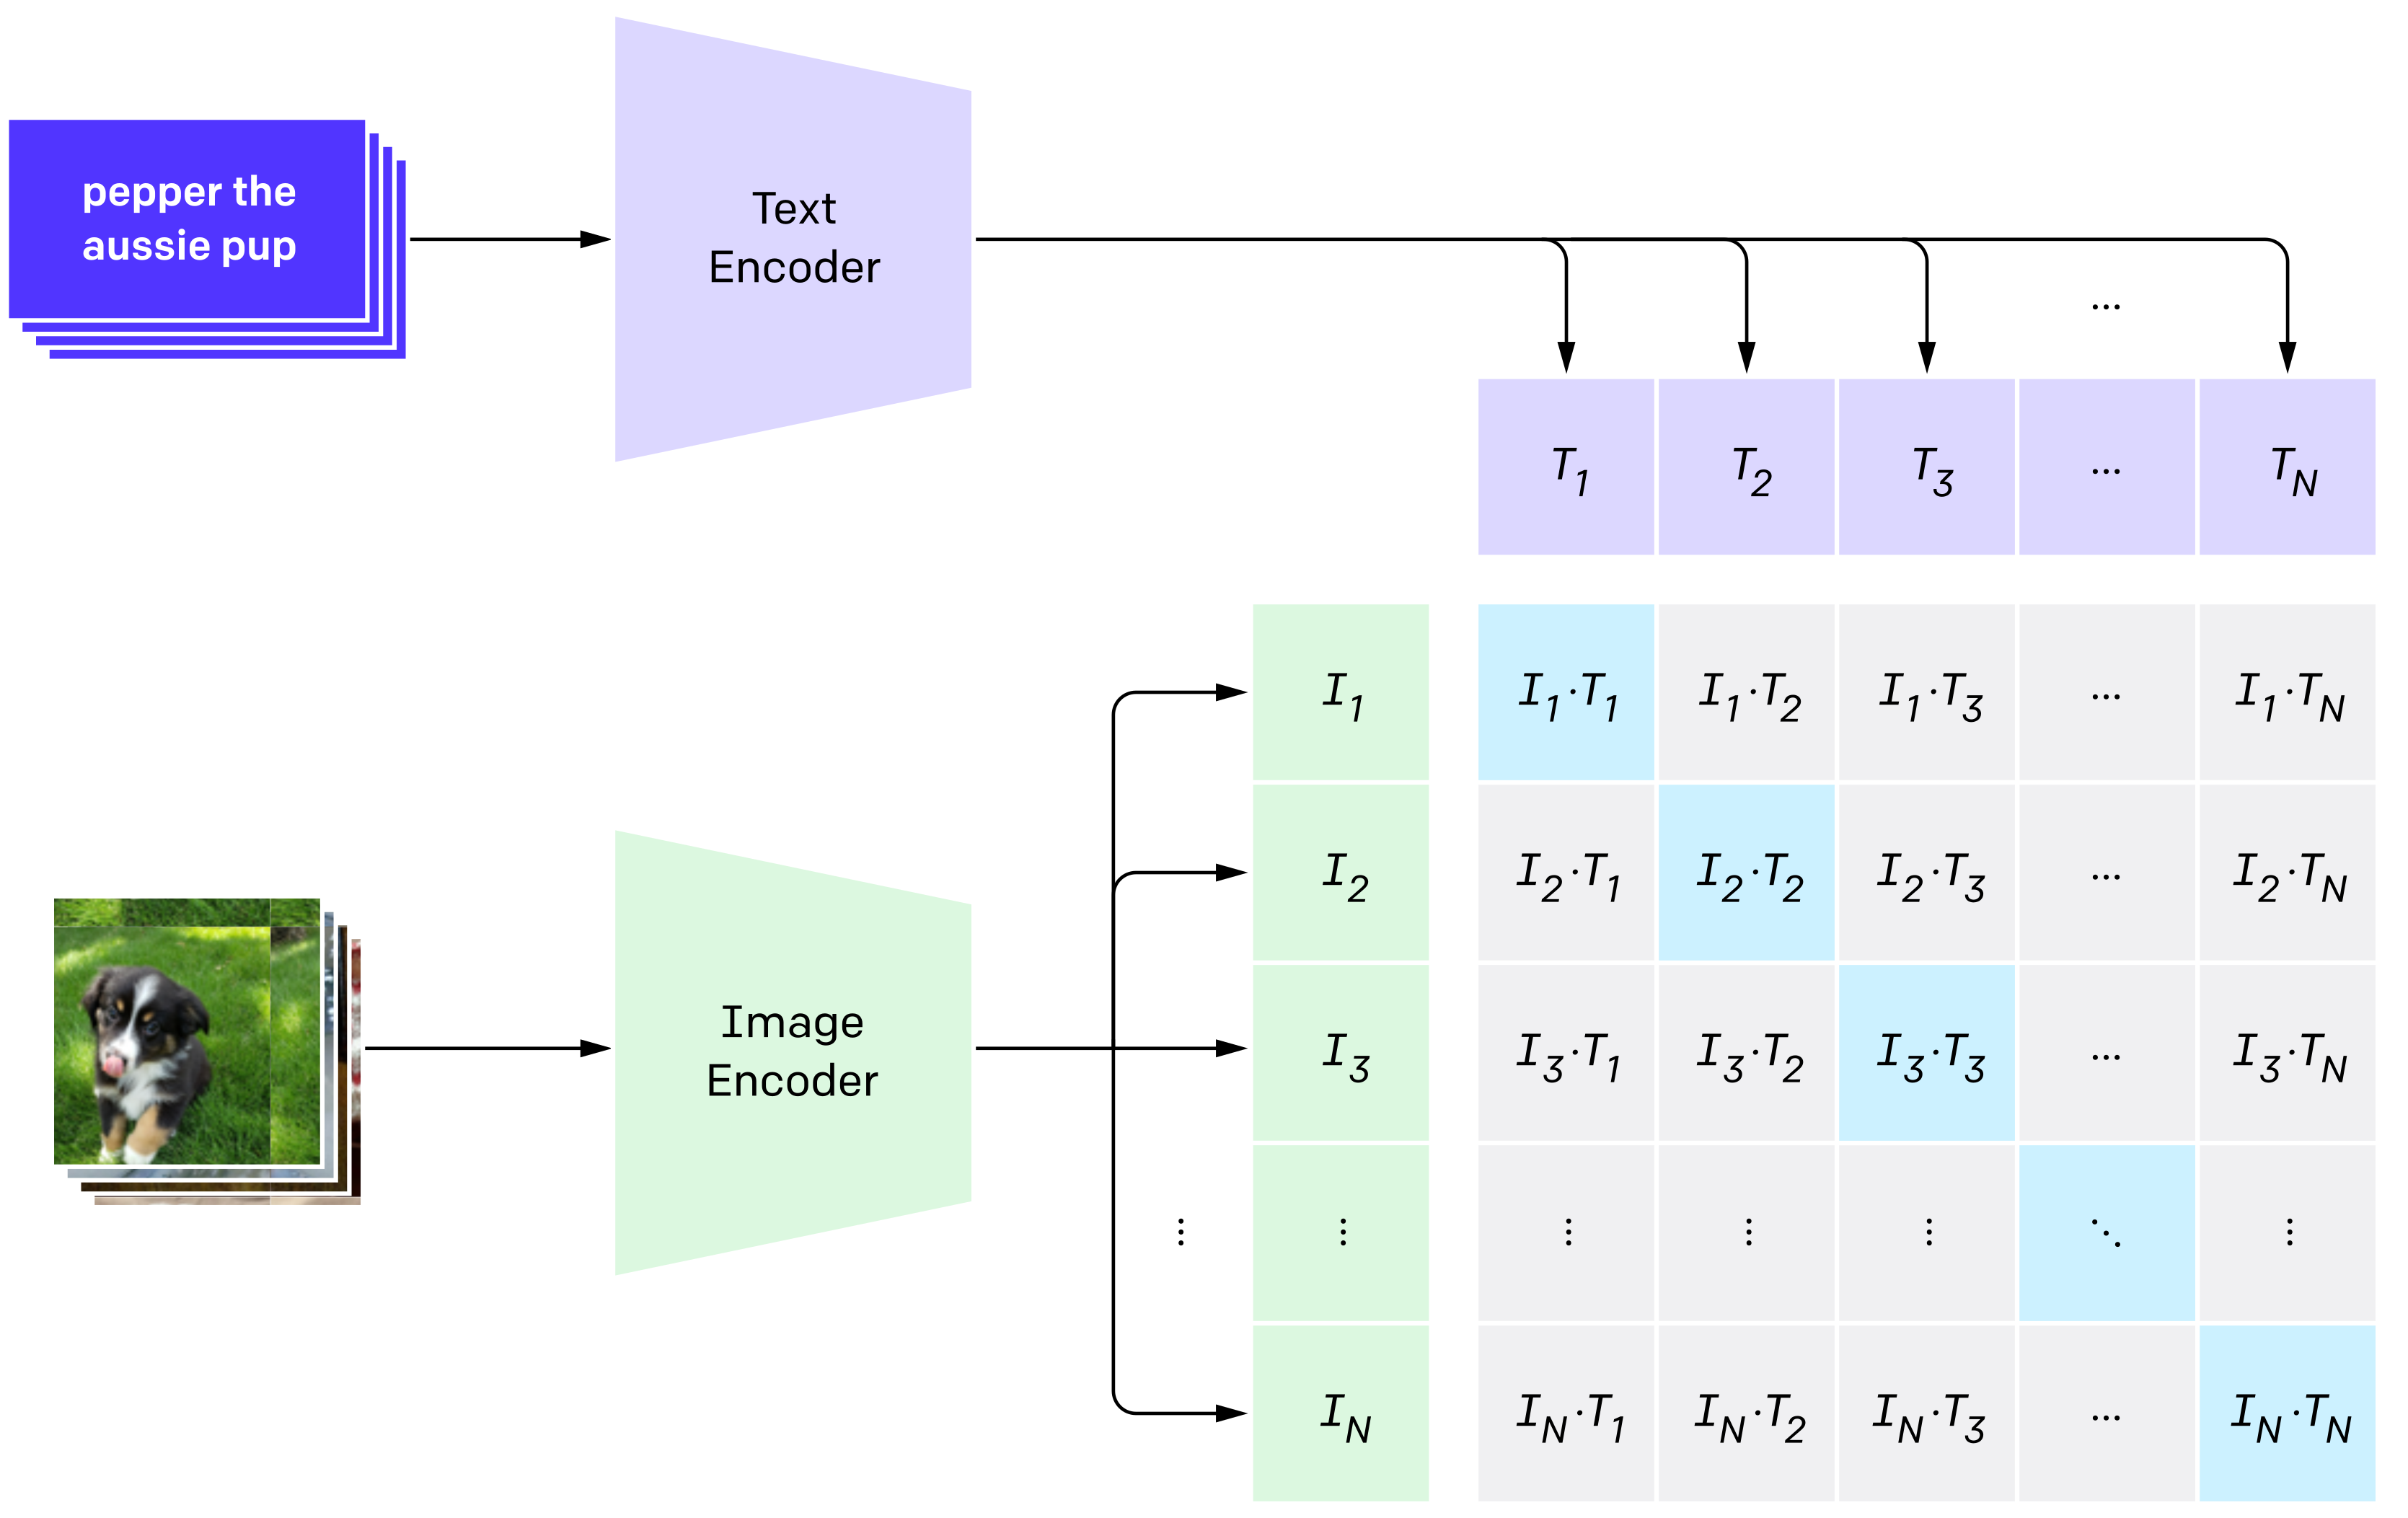
\includegraphics[width=\linewidth, keepaspectratio]{image/clip-a.png}
  \caption{CLIPの事前学習 \cite{clip}}
  \label{fig:clip-a}
\end{figure}
% 
CLIPは対照学習 (Contrastive Learning) と呼ばれる学習手法を採用しており,類似した特徴量間(正例)の類似度は大きく,類似していない特徴量間(負例)の類似度は小さくなるように学習が行われる.
具体的には,$N$個のテキストと画像のペアが入力され,画像エンコーダ (Image Encoder) やテキストエンコーダ (Text Encoder) によって,それぞれの特徴量が埋め込まれる.
$N$枚の画像から得られる特徴量は$I_1, I_2, \ldots, I_N$と,$N$個のテキストから得られる特徴量は$T_1, T_2, \ldots, T_N$と表される.
次に,埋め込まれた特徴量間のコサイン類似度が計算され,正例のコサイン類似度 $I_1 \cdot T_1, I_2 \cdot T_2, \ldots, I_N \cdot T_N$ を最大化し,負例のコサイン類似度を最小化するように画像エンコーダとテキストエンコーダのパラメータを更新する.
この対照学習により,CLIPは画像のみの学習では表現が困難であった,意味的な特徴抽出が可能となる.
また,CLIPは膨大な量の画像とテキストのペアを学習したことにより,タスク固有のデータセットによる追加学習を必要としないZero-Shotタスクに対して高いパフォーマンスを示すことが確認されている.

本研究では,テキストを用いた対照学習によって意味的な特徴表現が可能であるCLIPのIFORに対する有効性を検証する.
ただし,本研究では大規模なテキストと画像による対照学習が行われたCLIPモデルについて,画像エンコーダのみを特徴抽出器として採用する.

\subsection{転移学習}

一般的に,深層学習モデルは大規模なデータセットを用いた学習により高い汎化能力を獲得することが知られている.
一方で,学習用データを十分に確保できない場合,過学習が起こる可能性が高く,モデルが十分な汎化性能を得ることは極めて困難である.
実世界のタスクにおいては,多くの場合,大規模な学習データセットの構築が現実的に困難である.

これらの問題に対して,小規模なデータセットを用いて効率的にモデルの学習を行うFSLタスクでは,転移学習が重要な解決策として知られている.
図 \ref{fig:transfer_image}に転移学習の概要を示す.
% 
\begin{figure}[tbp]
  \centering
  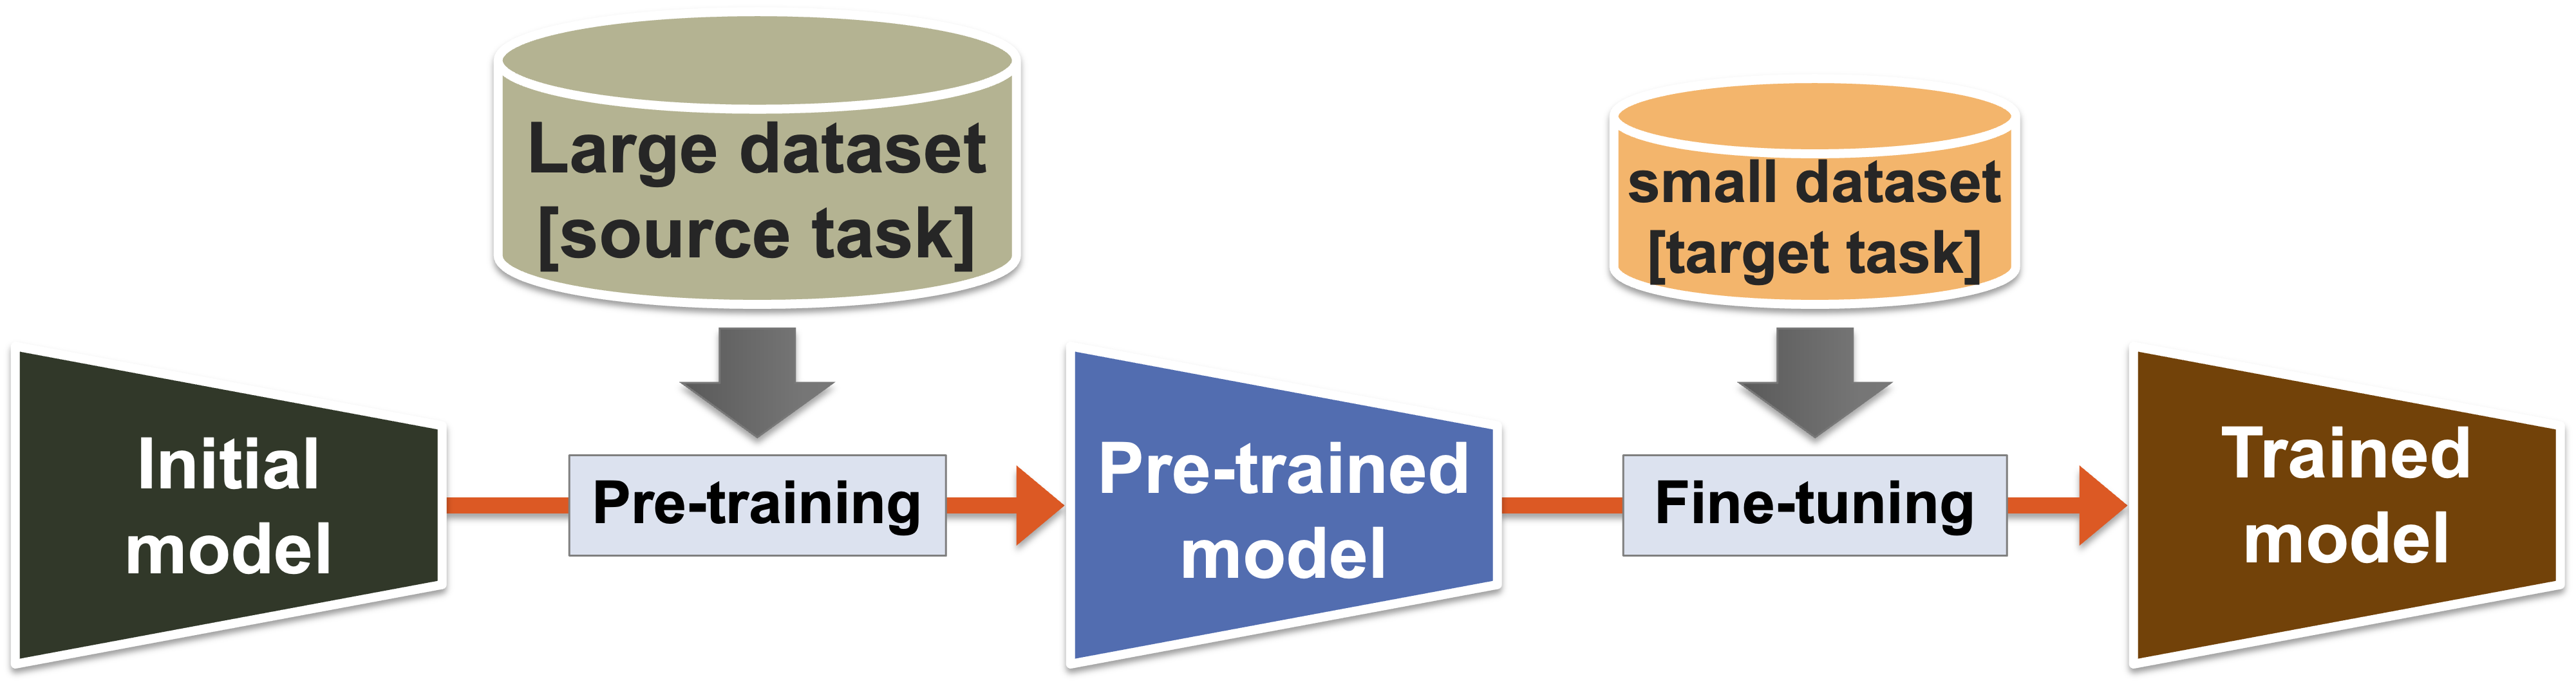
\includegraphics[width=\linewidth, keepaspectratio]{image/transfer_learning.png}
  \caption{転移学習の概要}
  \label{fig:transfer_image}
\end{figure}
% 
転移学習とは,事前に別のタスクから得られた知識を活用し,関連する新しいタスクに対して深層学習モデルの汎化性能を向上させる手法である.
この手法により,広範な学習データから得られた汎用的なモデルの知識を転移させることで,少量の学習データしかない場合においても深層学習モデルは高精度な分類が可能となる.

本研究ではIFORフレームワークにおける転移学習の有効性について検証を行う.
転移学習による性能向上において,事前学習のタスク(ソースタスク)と本番環境でのタスク(ターゲットタスク)の類似性は重要な要素である.
そこで,IFORのターゲットタスクが赤外線画像であることを考慮し,色情報を含まないフラクタル画像を事前学習に用いるFormula-Driven Supervised Learning (FDSL) \cite{fdsl}の適用可能性について評価を行う.
また,事前学習データセットとして様々な画像認識タスクで標準的に用いられており,包括的な画像を含んだ大規模データセットImageNetを用いた事前学習の有効性についても検証を行う.
図 \ref{fig:transfer_learning}に,それぞれのデータセットにおける画像の例を示す.
FDSLでは,数式によって生成されたフラクタル幾何画像を用いており,色情報が含まれないため,形状特徴を強調した特徴抽出器の学習が期待できる.

\begin{figure}[tbp]
  \centering
  \begin{subfigure}[b]{0.45\linewidth}
    \centering
    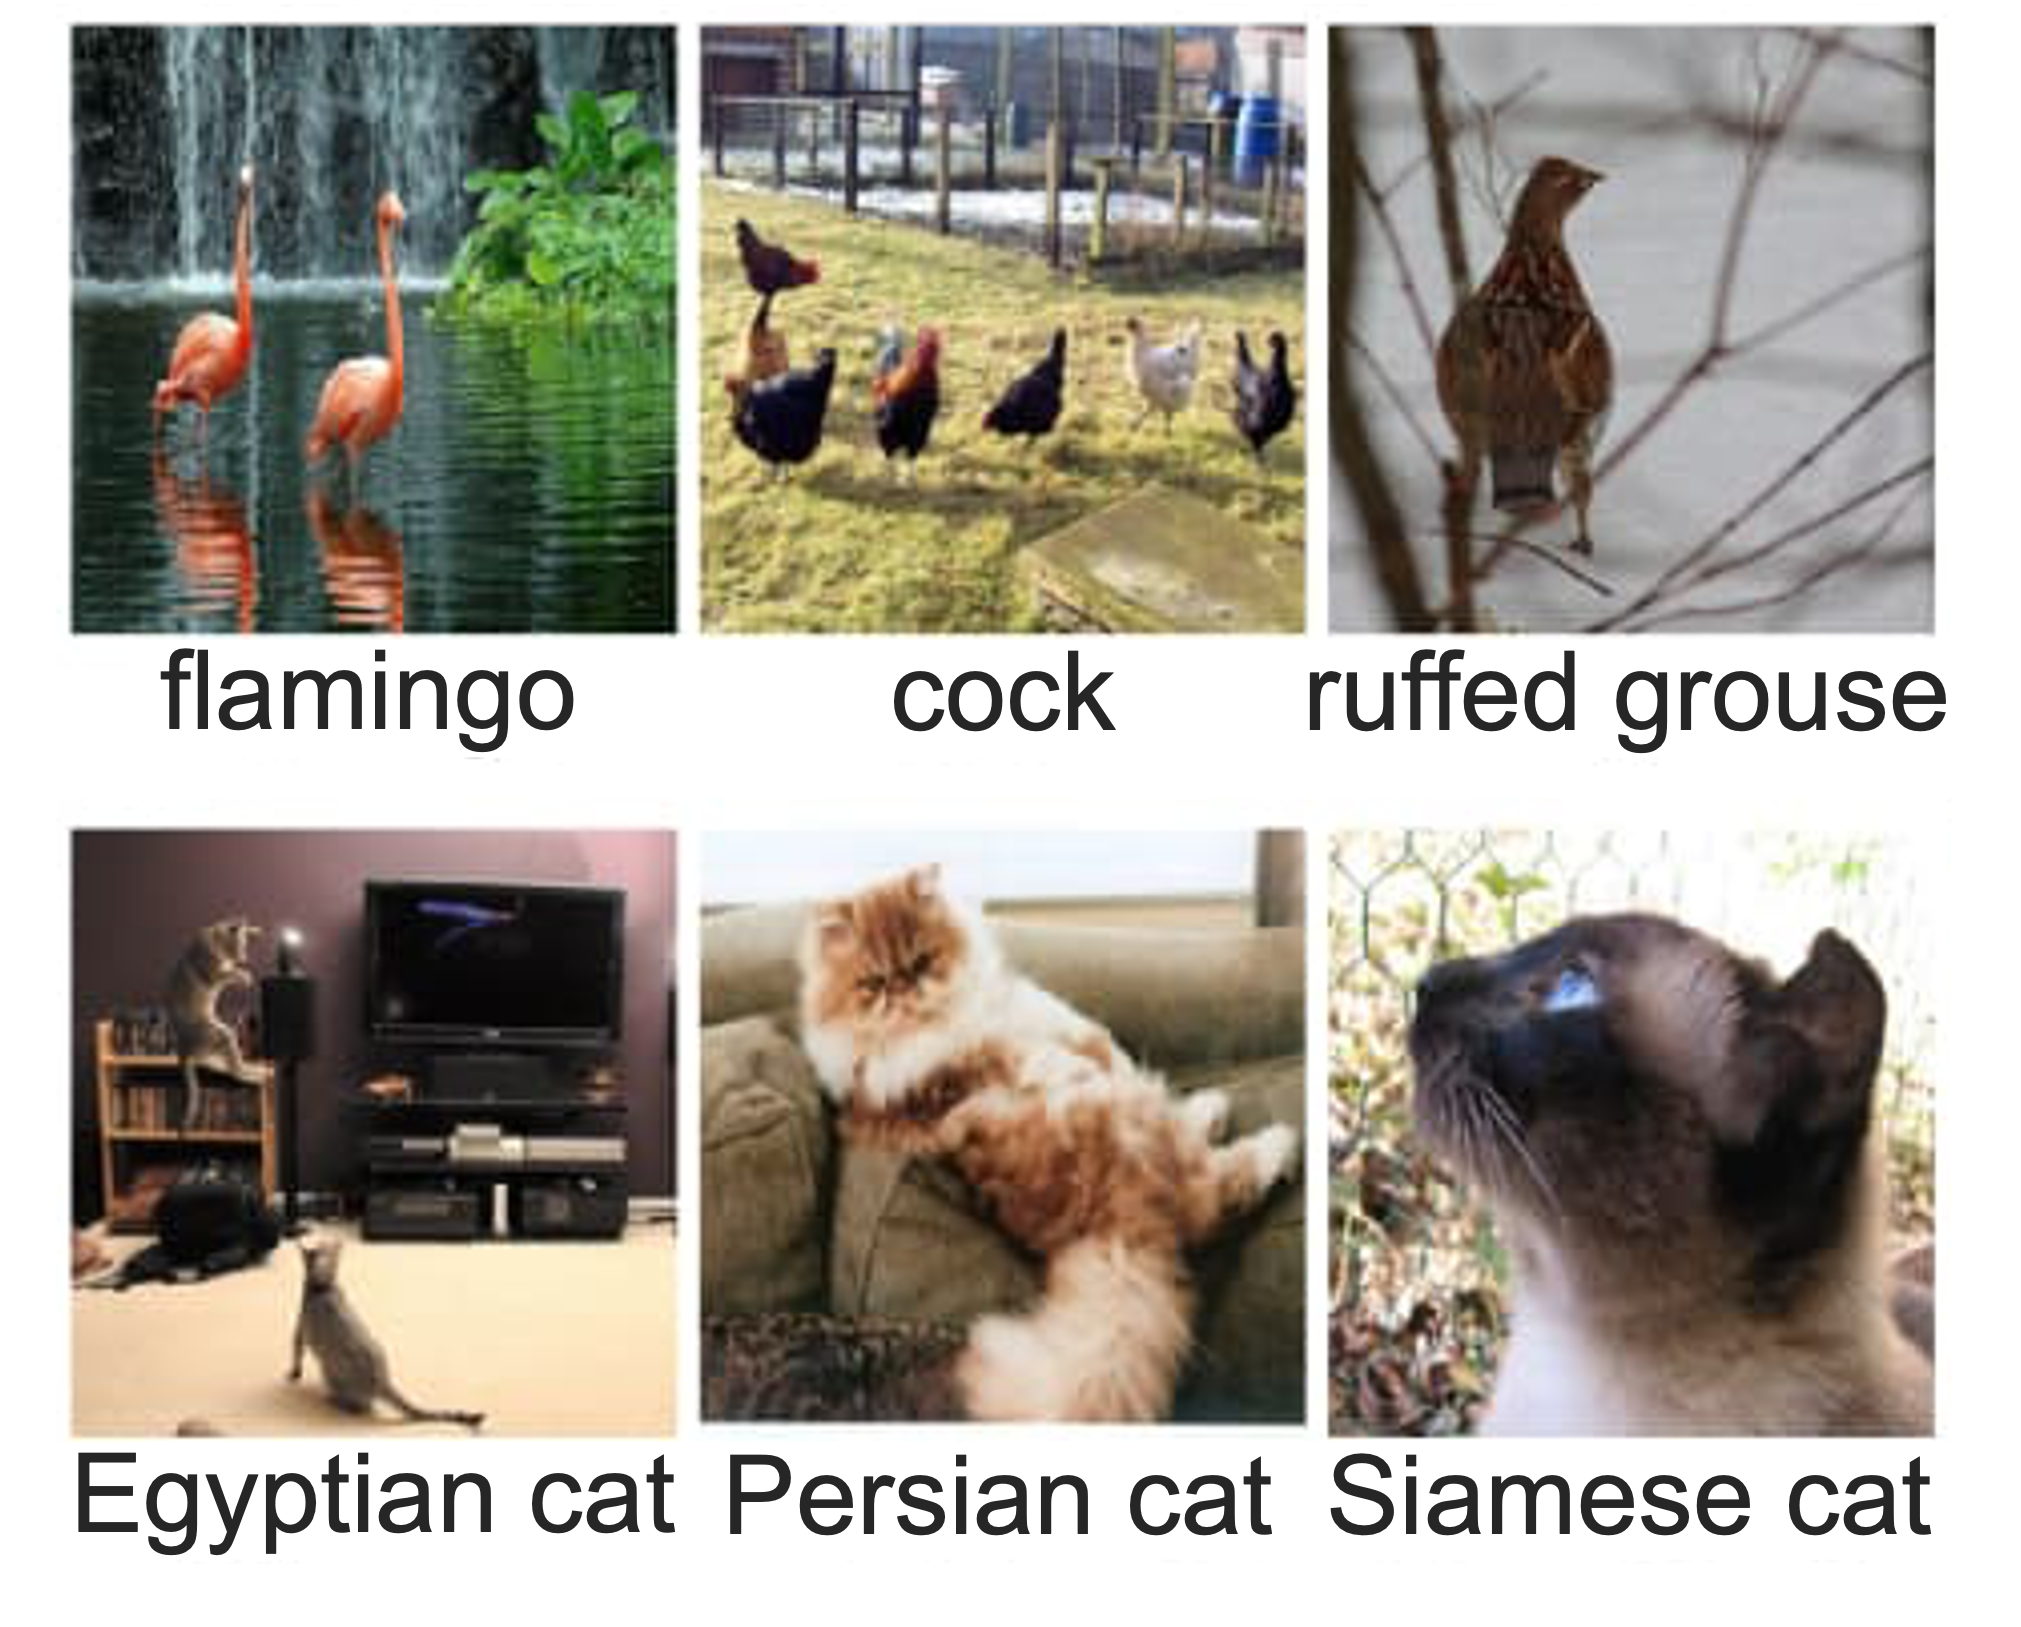
\includegraphics[height=0.9\linewidth, keepaspectratio]{image/imagenet.png}
    \caption{ImageNetの画像例}
    \label{fig:imagenet}
  \end{subfigure}
  \hfill
  \begin{subfigure}[b]{0.45\linewidth}
    \centering
    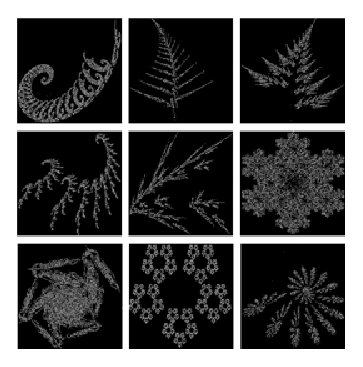
\includegraphics[height=0.9\linewidth, keepaspectratio]{image/fdsl.eps}
    \caption{FDSLの画像例}
    \label{fig:fdsl}
  \end{subfigure}
  \caption{ImageNetとFDSLの画像例}
  \label{fig:transfer_learning}
\end{figure}

\subsection{メタ学習}

メタ学習は,学習方法の学習として知られており,FSLにおける効率的なアプローチとして広く認識されている.
図 \ref{fig:meta-learning}にメタ学習の概要図を示す.
% 
\begin{figure}[tbp]
  \centering
  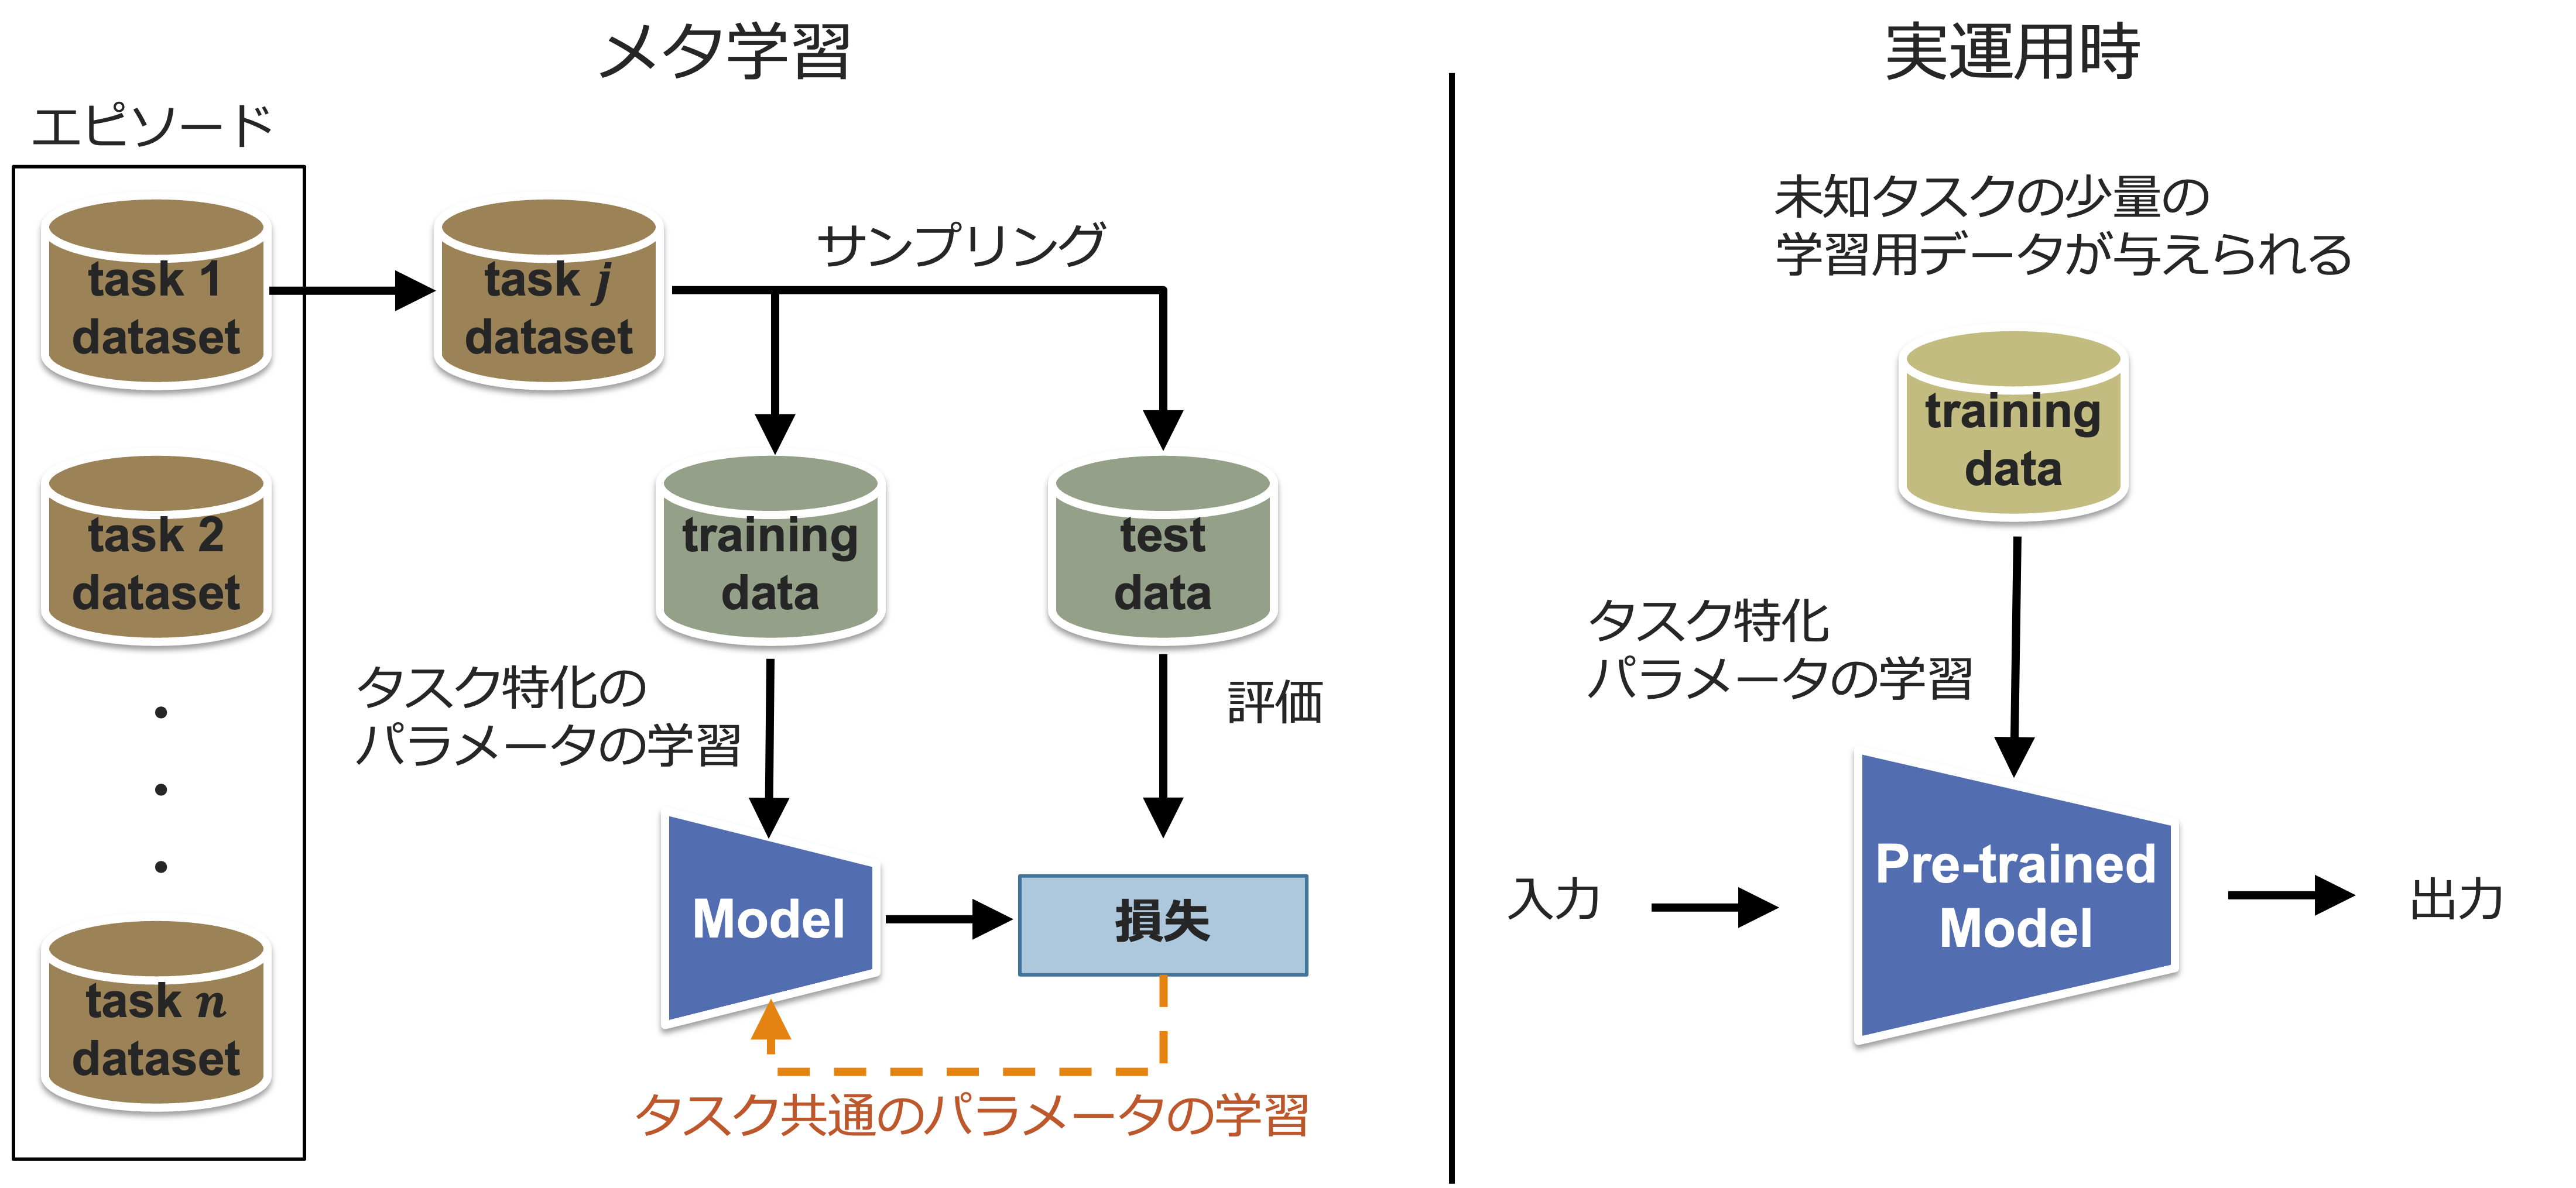
\includegraphics[width=\linewidth, keepaspectratio]{image/meta-learning.png}
  \caption{メタ学習の概要}
  \label{fig:meta-learning}
\end{figure}
% 
メタ学習では,様々なタスクによって構成される学習単位をエピソードと呼び,深層学習モデルは複数のエピソードを通じて学習アルゴリズムを改善し,
限られたデータに対する汎化性能を強化する.
各タスクは,それぞれ$K$個のデータを持つ$N$個のクラスで構成されており,このタスク設定は``$N$-Way, $K$-Shot分類''と呼ばれる.

メタ学習の各エピソードでは,ランダムに選択された学習タスクに基づいてモデルパラメータが更新される.
このプロセスにより,モデルは各エピソードで異なるタスクへの対応を求められ,特定のサブセットではなくより一般的な特徴表現の獲得が期待される.

Snellらは,FSLの代表的なメタ学習手法であるPrototypical Networks (ProtoNet) を提案した \cite{protonet}.
ProtoNetの概要を図 \ref{fig:protonet}に示す.
% 
\begin{figure}[tbp]
  \centering
  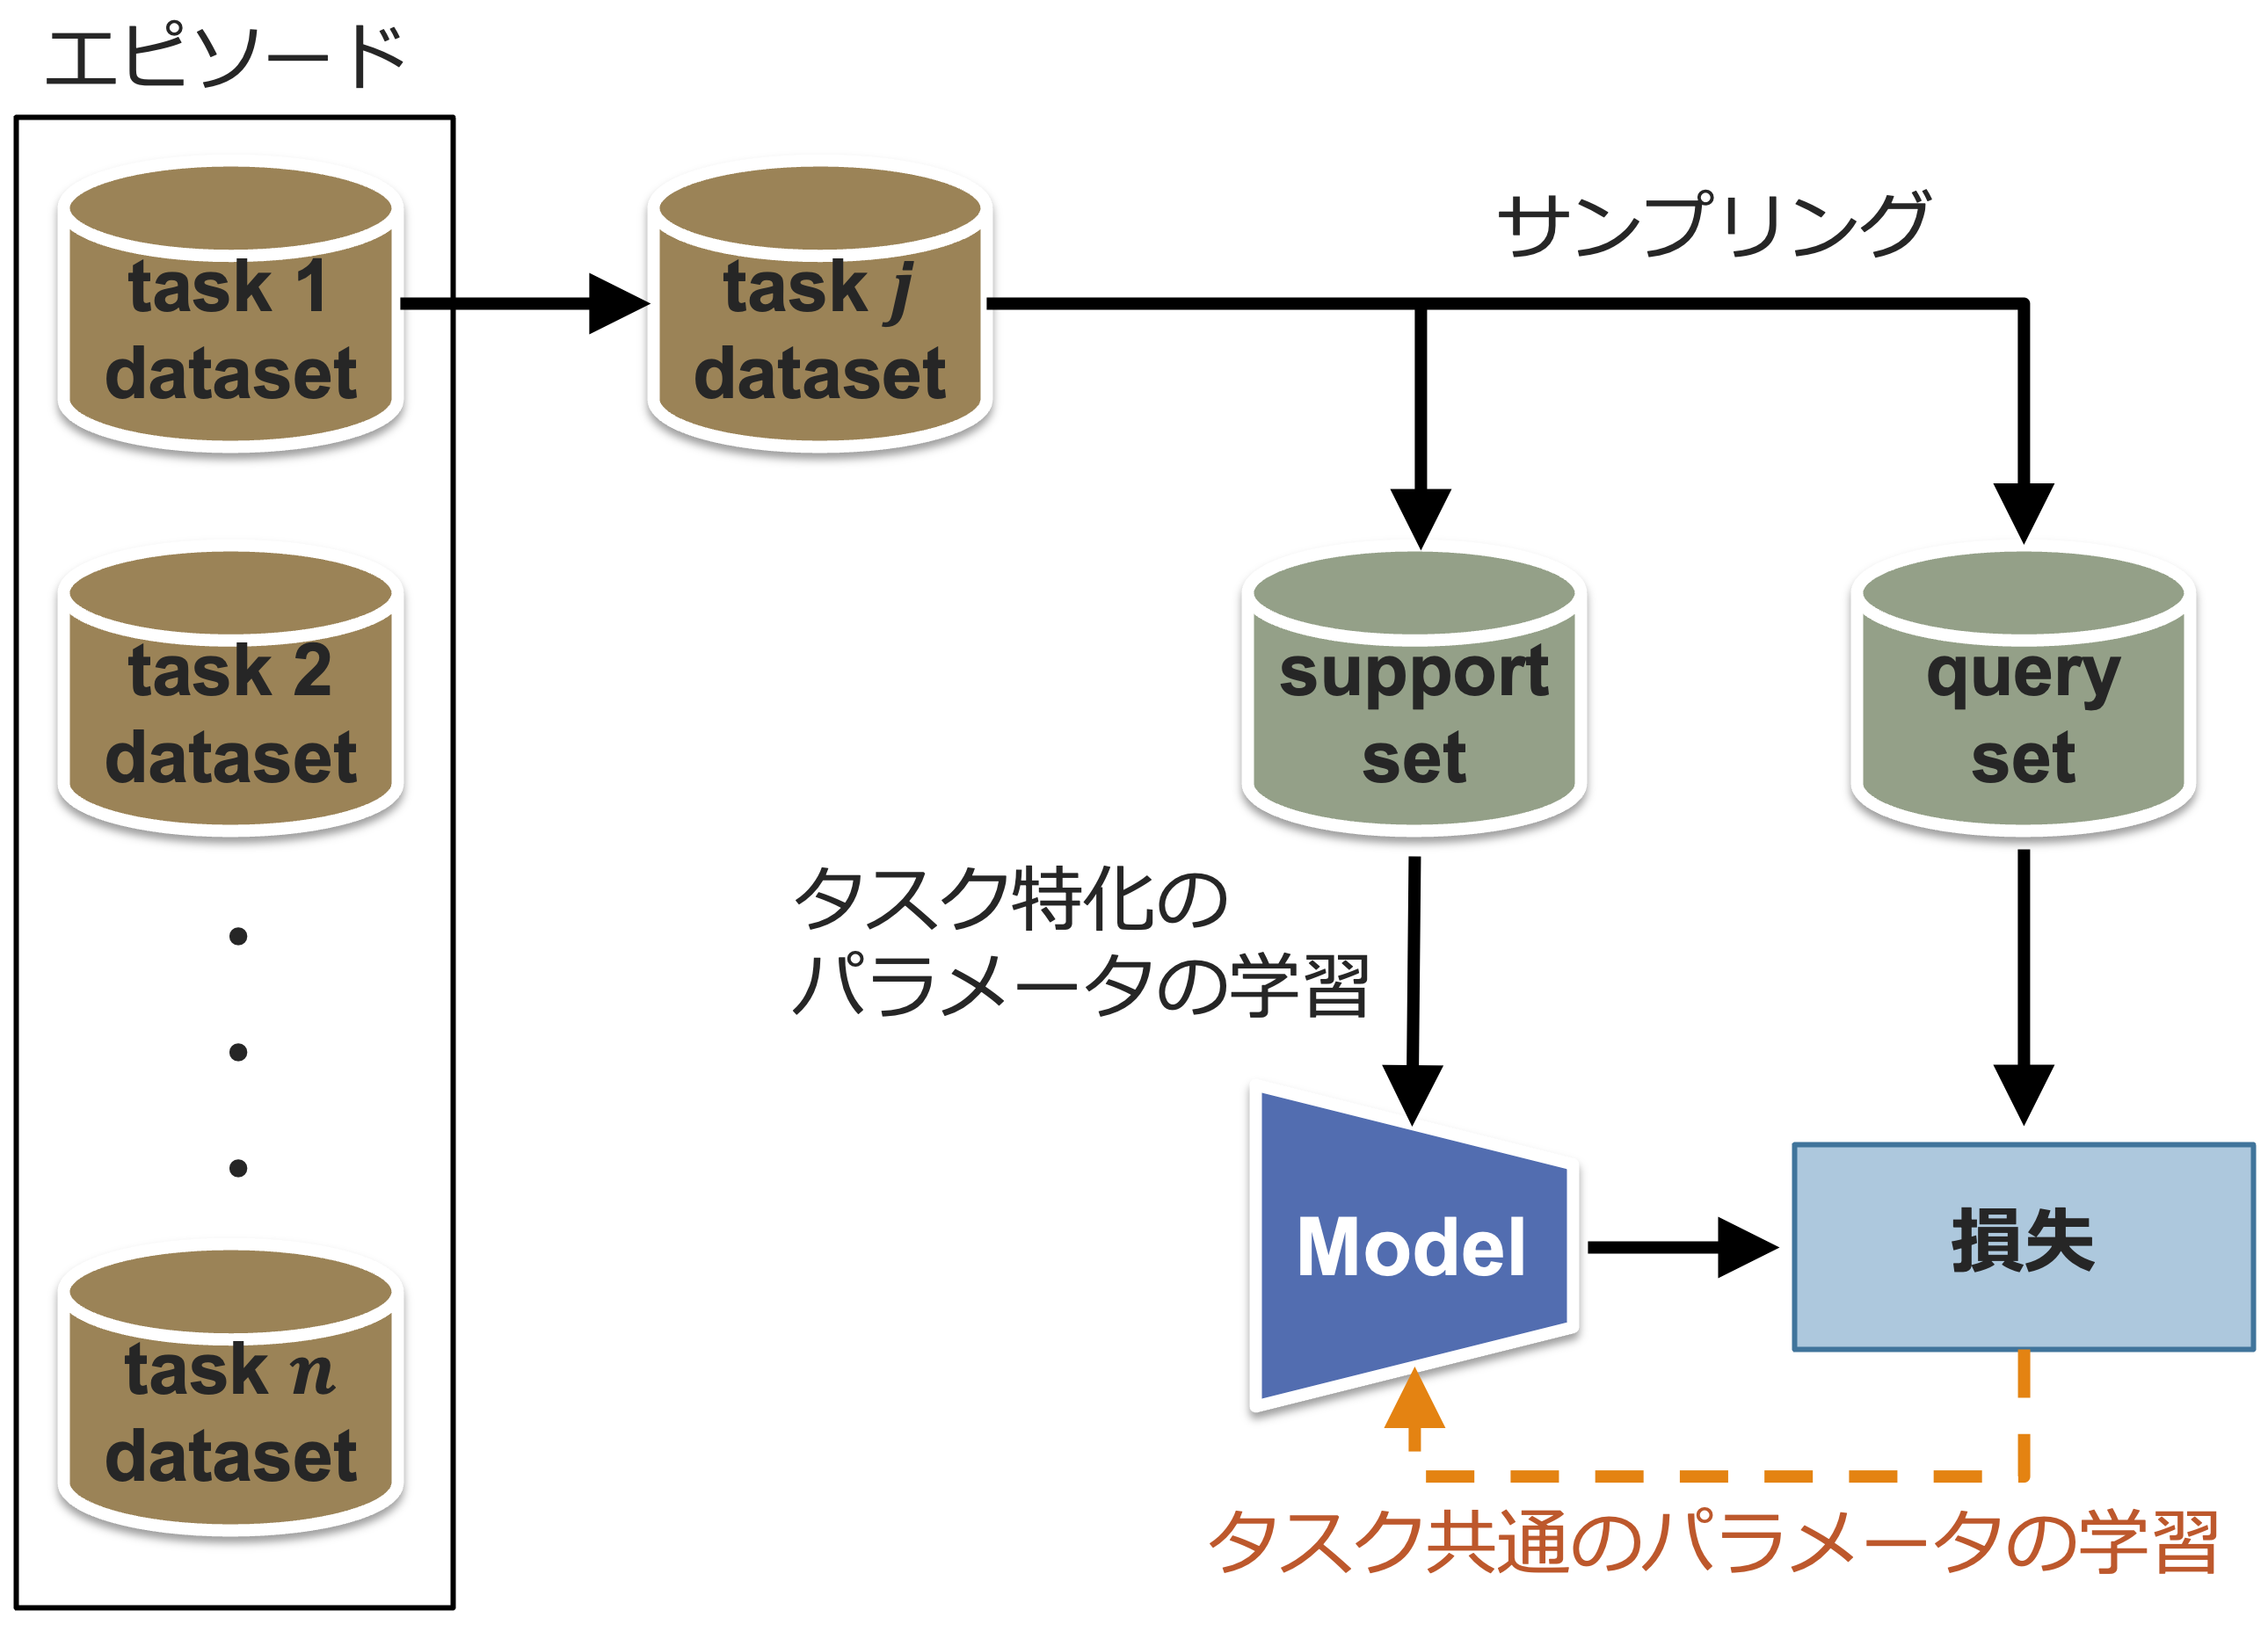
\includegraphics[width=0.7\linewidth, keepaspectratio]{image/protonet.png}
  \caption{ProtoNetの概要}
  \label{fig:protonet}
\end{figure}
% 
ProtoNetでは,モデルに登録するクラスセットであるサポートセット (support-set) と,サポートセットを評価するためのクエリセット (query-set) を用いて学習を行う.
ProtoNetは,入力データと各クラスのプロトタイプとの距離に基づいて分類のための特徴空間を学習し,少数データにおける分類を実現する.
プロトタイプはサポートセットの埋め込みベクトルの平均として定義される.
具体的に,サポートデータは各クラスのプロトタイプを中心としたクラスタを形成するような空間に埋め込まれ,
分類時には,クエリデータの埋め込みベクトルに最も近いプロトタイプを持つクラスが予測クラスとして分類される.
このような距離に基づく分類手法により,FSLにおいて課題となる過学習に対処している.

近年,メタ学習アルゴリズムがFew-Shot Open-Set Recognition (FSOSR) の分野に拡張され,
登録クラスの分類と未登録クラスの検出の両方を同時に高い精度で実現する手法が提案された.
Liuらは,モデルの学習過程で登録クラスの分類と未登録クラスの検出に取り組むPEELERアルゴリズムを提案した \cite{peeler}.
従来のソフトマックス分類器は,学習クラスを過剰に適合させる傾向があるため,未登録クラスの検出が困難であった.
PEELERはこの課題に対し,エピソードごとに新規クラスをランダムに選択し,これらのクラスの事後エントロピーを最大化することにより未登録クラスの検出能力の向上を図っている.
さらに,メタ学習をオープンセット認識に拡張したことにより,より一般化された特徴抽出における表現力を獲得し,
認識タスクの様々なスケールや複雑さに対して効果的な学習フレームワークを提供する.

PELLERの概要を図 \ref{fig:peeler}に示す.
% 
\begin{figure}[tbp]
  \centering
  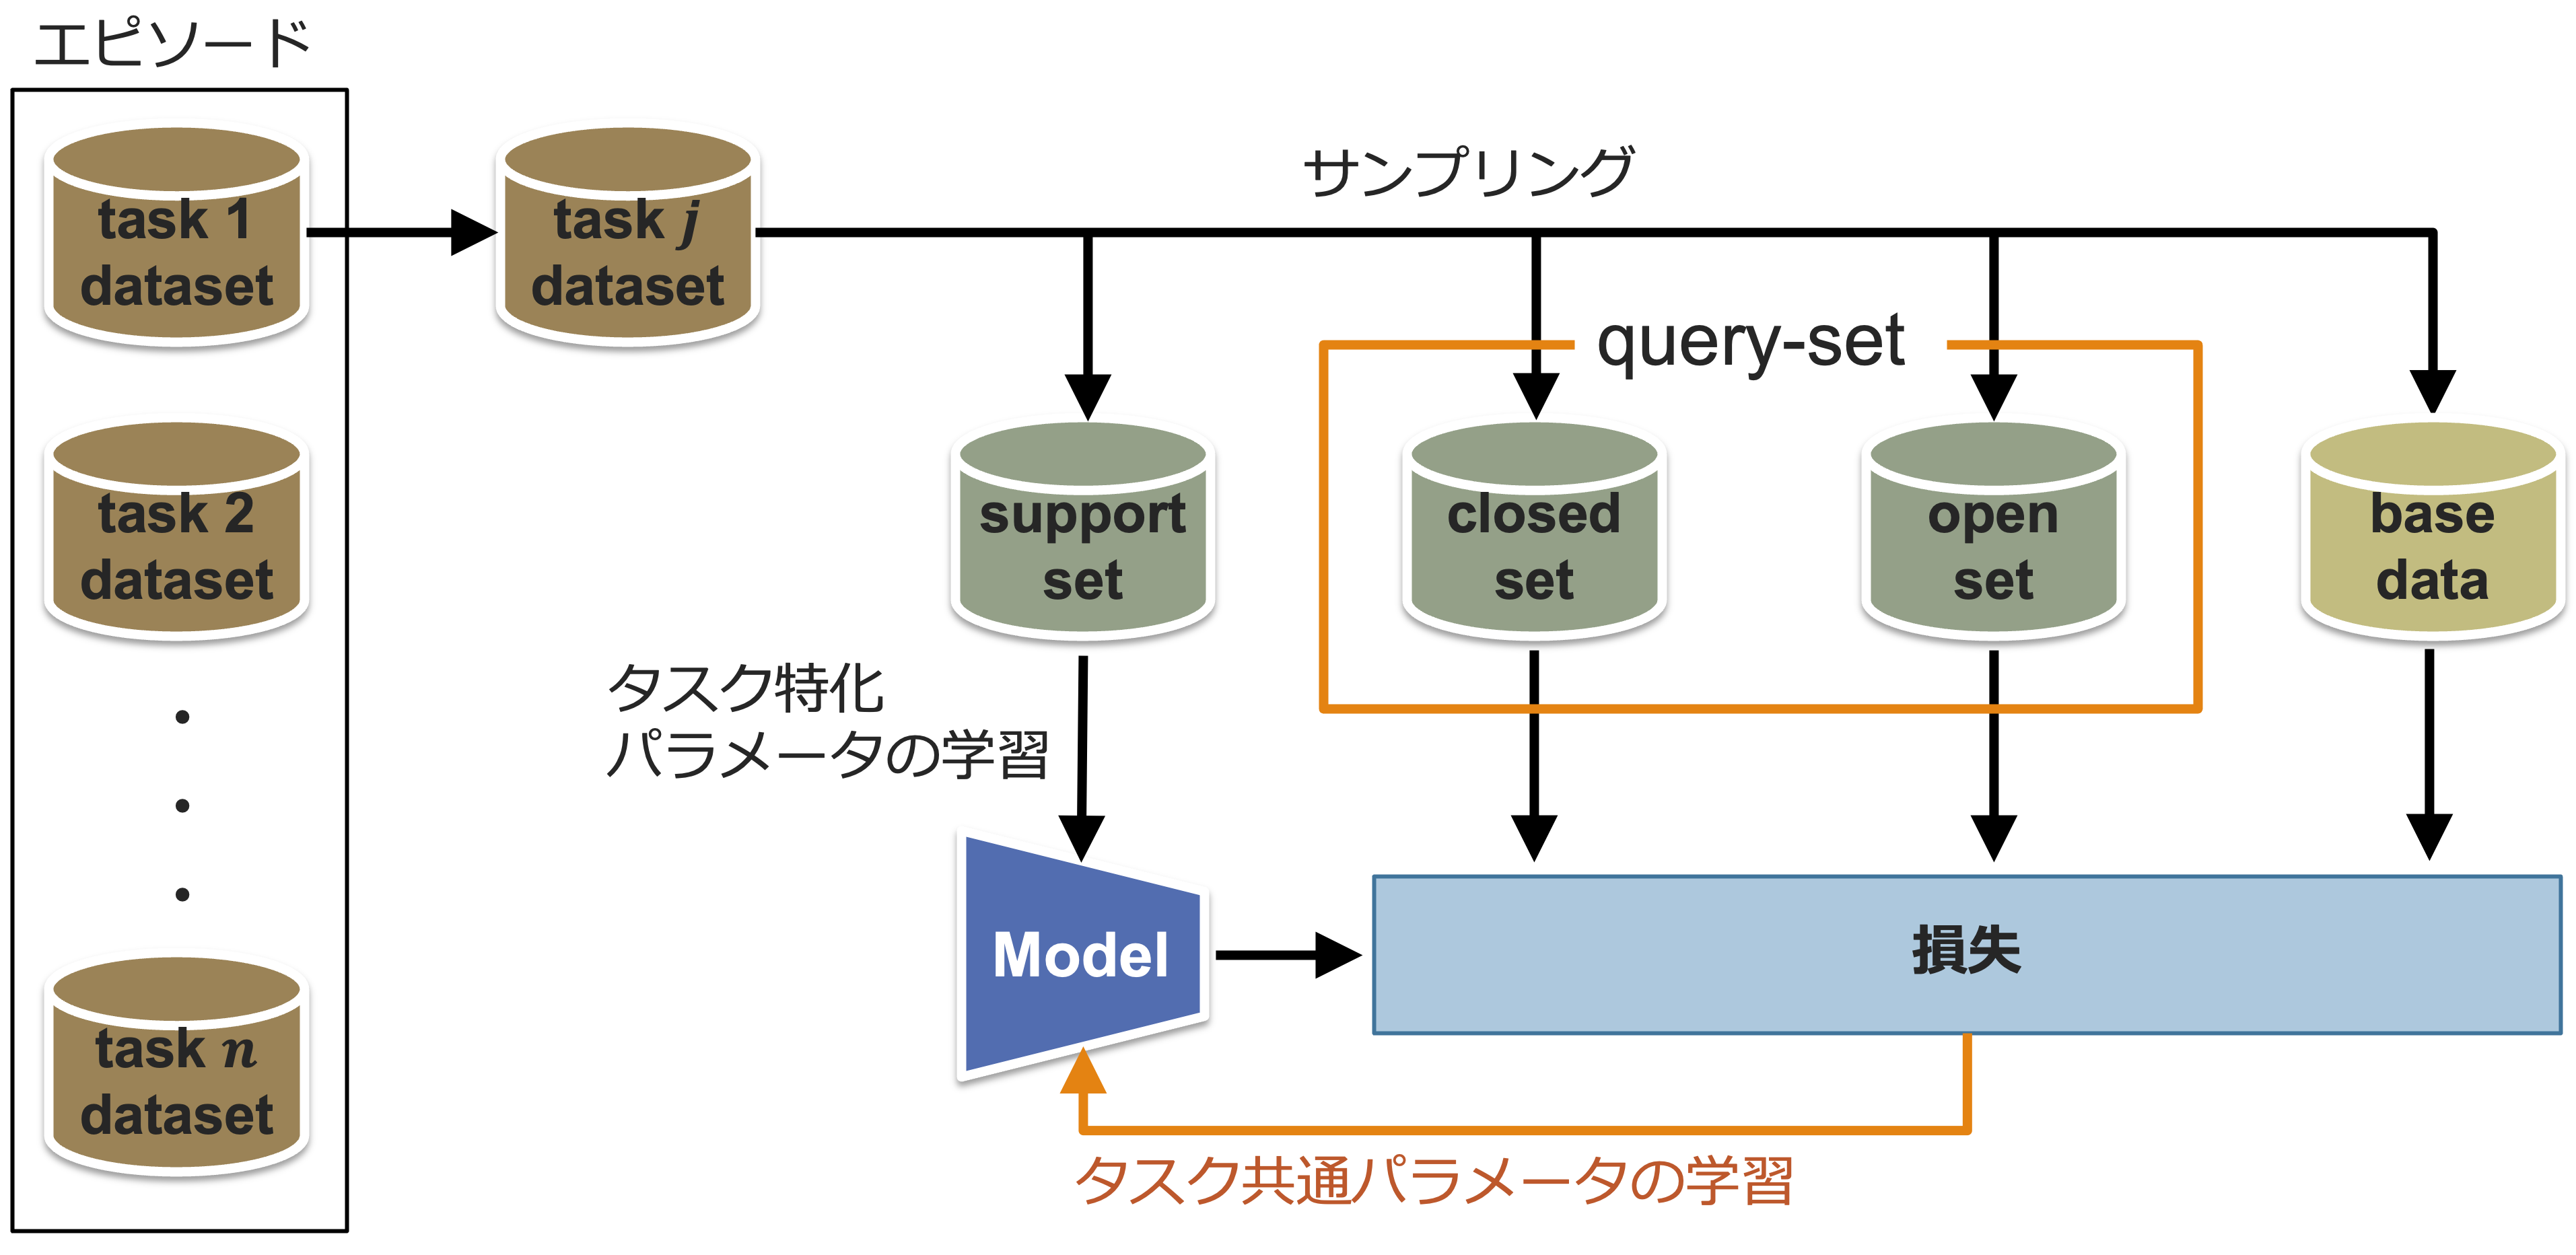
\includegraphics[width=\linewidth, keepaspectratio]{image/peeler.png}
  \caption{PEELERの概要}
  \label{fig:peeler}
\end{figure}
% 
各タスクではサポートセット (support-set) と呼ばれる登録用データとクエリセット (query-set) と呼ばれる評価用データを使用する.
$N$-Way, $K$-Shot分類におけるサポートセットは$\mathcal{D}^S = \left\{ \bm{x}^S_i, y^S_i \right\}^{NK}_{i=1}$と表される.
ここで,$\bm{x}^S_i \in \mathcal{X}^S$はサポートセットの入力画像空間$\mathcal{X}^S$における入力画像であり,$y^S_i \in \mathcal{Y}^S$は登録クラス空間$\mathcal{Y}^S$における教師ラベルを示す.
また,$N$はサポートセットのクラス数,$K$は各クラスのサンプル数を表す.
さらに,クエリセットはサポートセットと同じクラスから構成されるクローズドクエリセット (closed-query set) と,
サポートセットと異なるクラスから構築されるオープンクエリセット (open-query set) の2つに分けられる.
クローズドクエリセットは$\mathcal{D}^C = \left\{ \bm{x}^C_i \in \mathcal{X}^C, y^C_i \in \mathcal{Y}^S \right\}^{NQ}_{i=1}$と表される.
ここで,$\bm{x}^C_i$はクローズドクエリセットの入力画像空間$\mathcal{X}^C$における入力画像であり,$y^C_i$は登録クラス空間$\mathcal{Y}^S$における教師ラベルを示す.
また,$N$はクローズドクエリセットのクラス数,$Q$は各クラスのサンプル数を表す.
一方で,オープンクエリセットは$\mathcal{D}^O = \left\{ \bm{x}^O_i \in \mathcal{X}^O, y^O_i \in \mathcal{Y}^O \right\}^{N^U}_{i=1}$と表される.
ここで,$\bm{x}^O_i$はオープンクエリセットの入力画像空間$\mathcal{X}^O$における入力画像であり,$y^O_i$は未登録クラス空間$\mathcal{Y}^O$における教師ラベルを示す.
また,オープンクエリセットはモデルに未登録のデータ集合であるため$\mathcal{Y}^S \cap \mathcal{Y}^O = \emptyset$ が成り立つ.
サポートセットやクローズドクエリセットがクラス数を明示的に定義するのに対し,オープンクエリセットは未登録クラスの検出を目的とするため,クラス数を定義せず総サンプル数$N^U$のみで表される.
PEELERではこの未登録クラスを単一クラスとして定義することにより,未登録クラスの検出に焦点を当てている.
サポートデータ,クローズドクエリデータ,オープンクエリデータの選択方法の概要を図 \ref{fig:peeler_data}に示している.
% 
\begin{figure}[tbp]
  \centering
  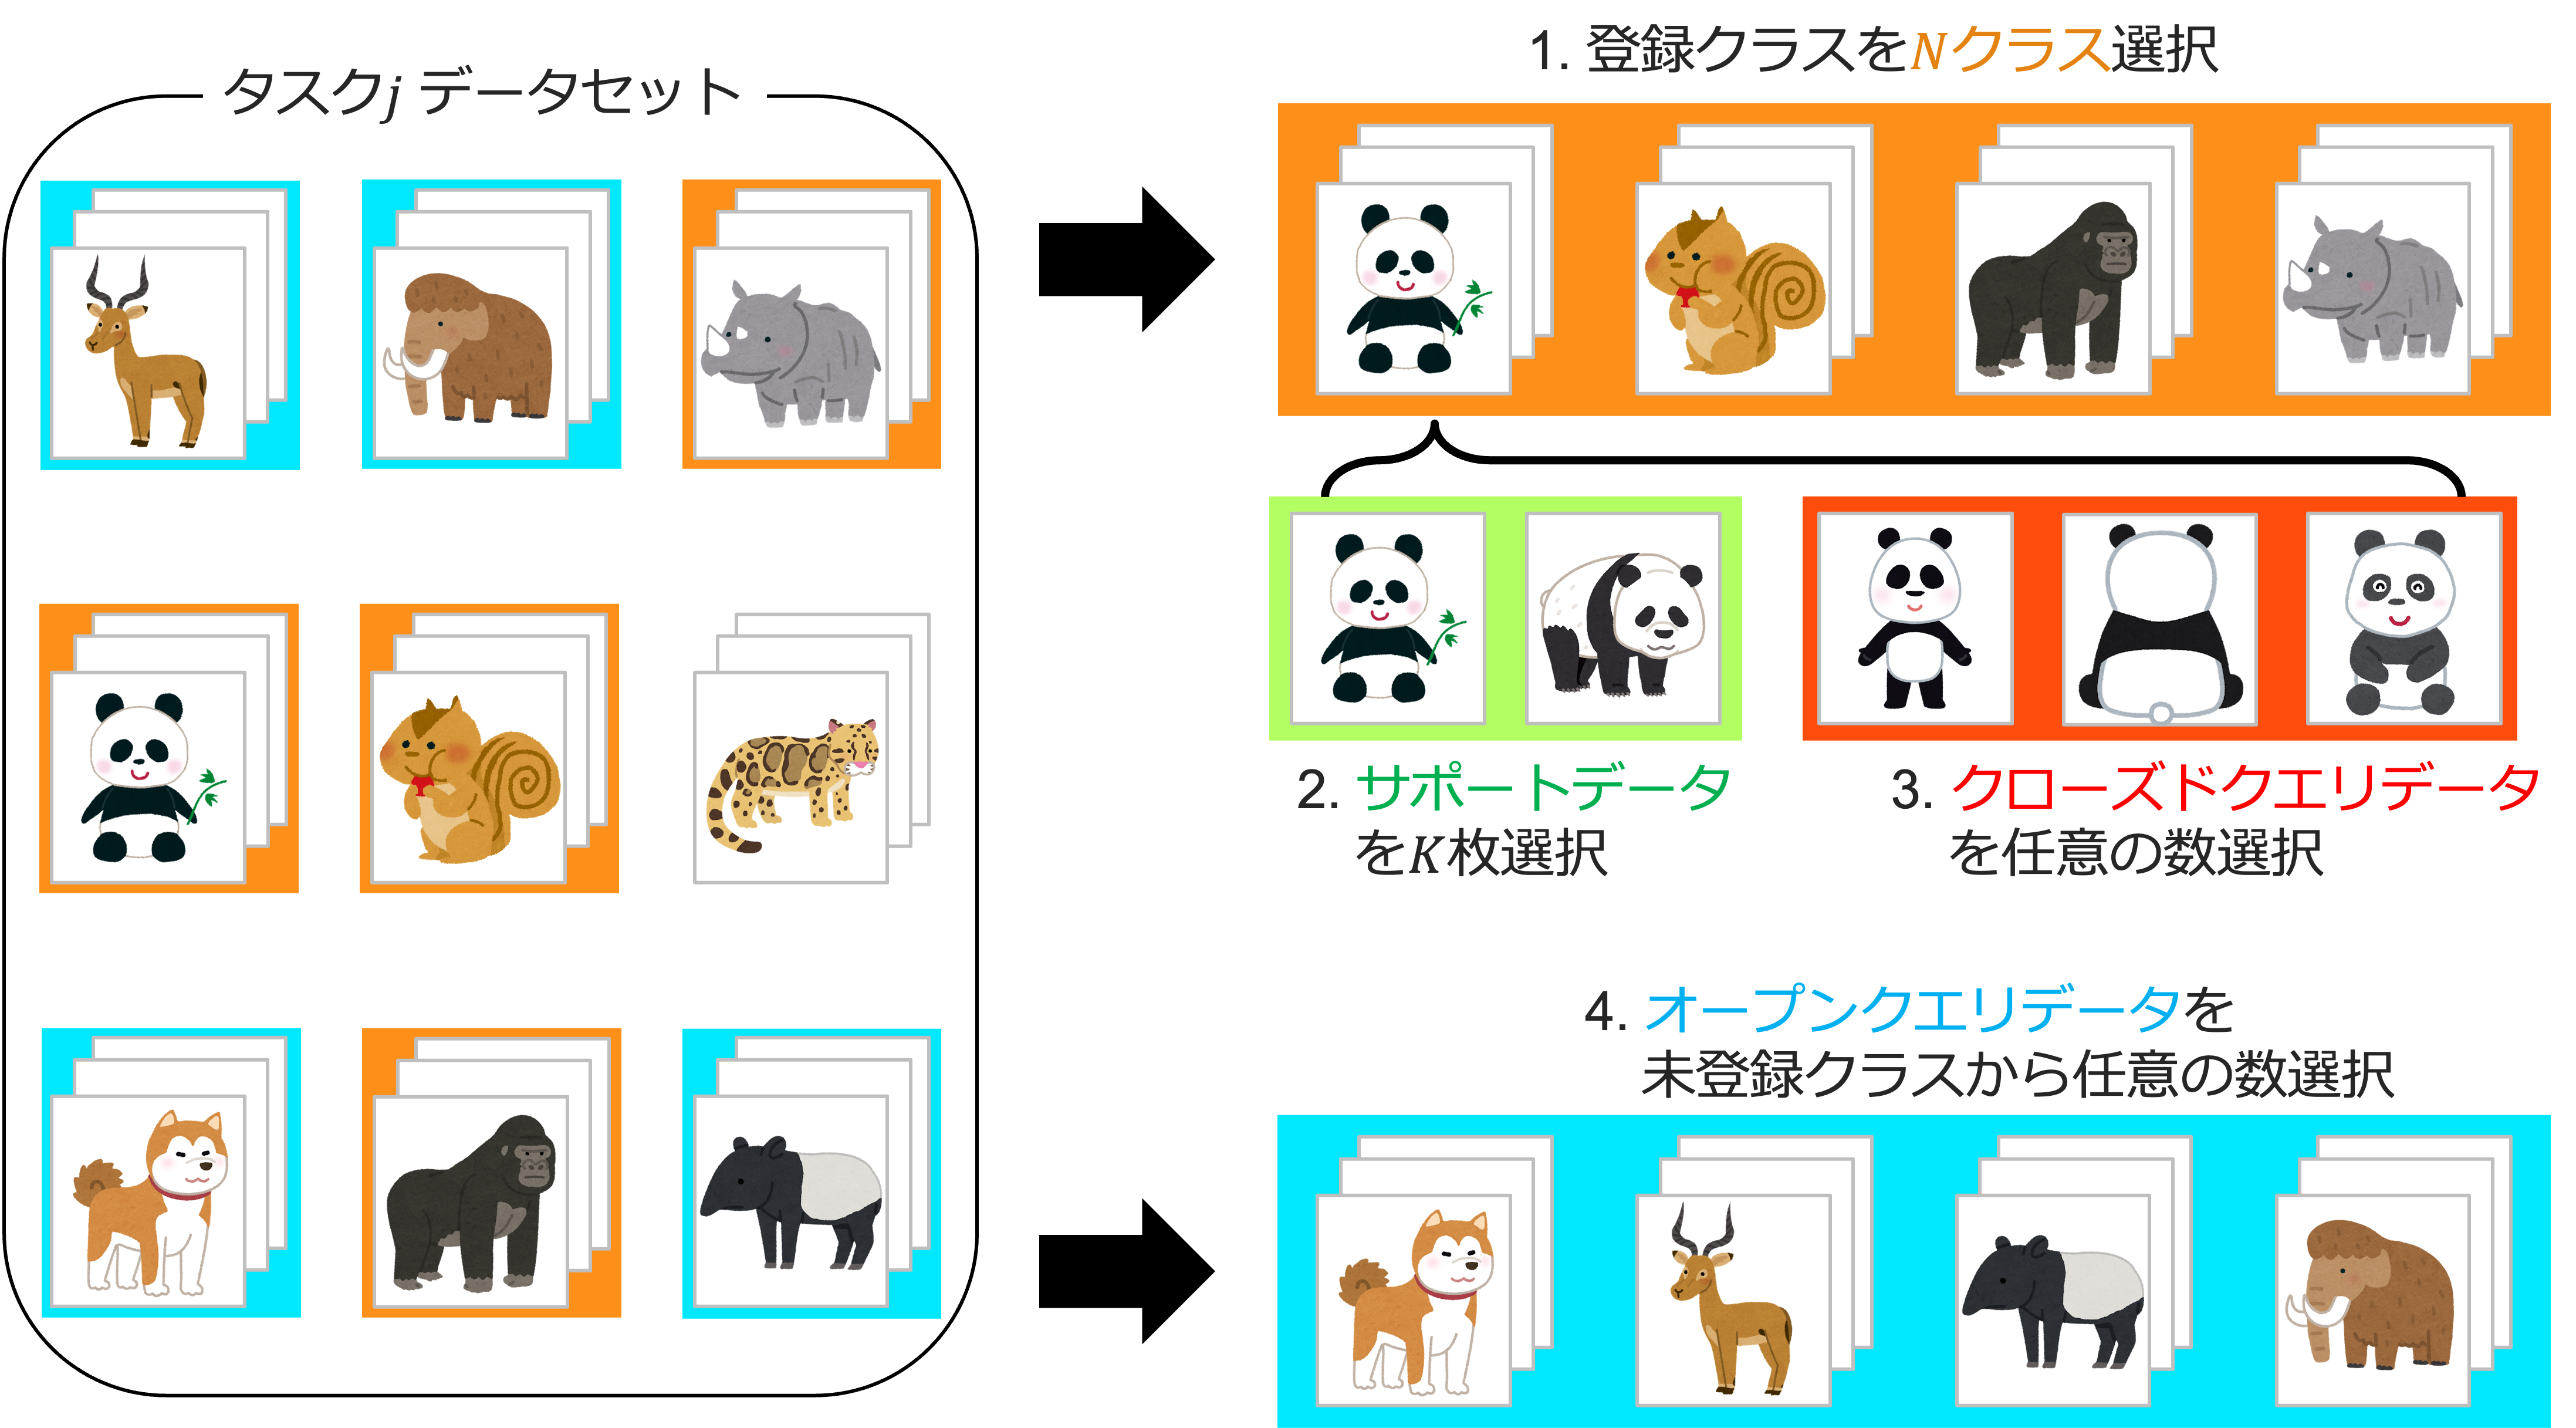
\includegraphics[width=\linewidth, keepaspectratio]{image/meta-class.png}
  \caption{登録クラス・未登録クラスの選択方法}
  \label{fig:peeler_data}
\end{figure}
%
PEELERは,プロトタイプと入力データとの距離に基づいて分類を行う.
具体的には,クエリデータが各プロトタイプの閾値より大きい場合は未登録クラス,閾値よりも小さい場合は最も近いプロトタイプのクラスに分類される.
PEELERはモデルに登録されたクラスの分類と未登録クラスの検出において高い精度を達成するため,FSL損失,OSR損失,分類損失の3つの異なる損失関数を採用している.
FSL損失は,プロトタイプとクローズドクエリセットを近づけることで,少数データにおける登録クラスの分類性能を向上させる.
OSR損失はプロトタイプとオープンクエリセットを離すことで,未登録クラスの検出精度を向上させる.
最後に,分類損失は,ランダムな画像から構成されるベースデータから適切な特徴を抽出し,モデルの分類能力を最適化するように設計されている.
エピソードを通してタスク間で異なるクラスセットを学習することにより,モデルは特定のタスクではなく,タスク間の共通性を学習することが期待される.

FSL損失の導出には,学習用データセットから選択されるサポートセットとクローズドクエリセットが用いられる.
メタ学習の過程において,クローズドクエリデータから抽出された特徴ベクトルをサポートデータの正解クラスに近づける学習を行うことで,
モデルは正確な分類を実現する特徴マッピングが習得可能となる.
図\ref{fig:fsl_loss}では,FSL損失で学習することにより効果的に登録クラスの分類が可能になる例を示している.
% 
\begin{figure}[tbp]
  \centering
  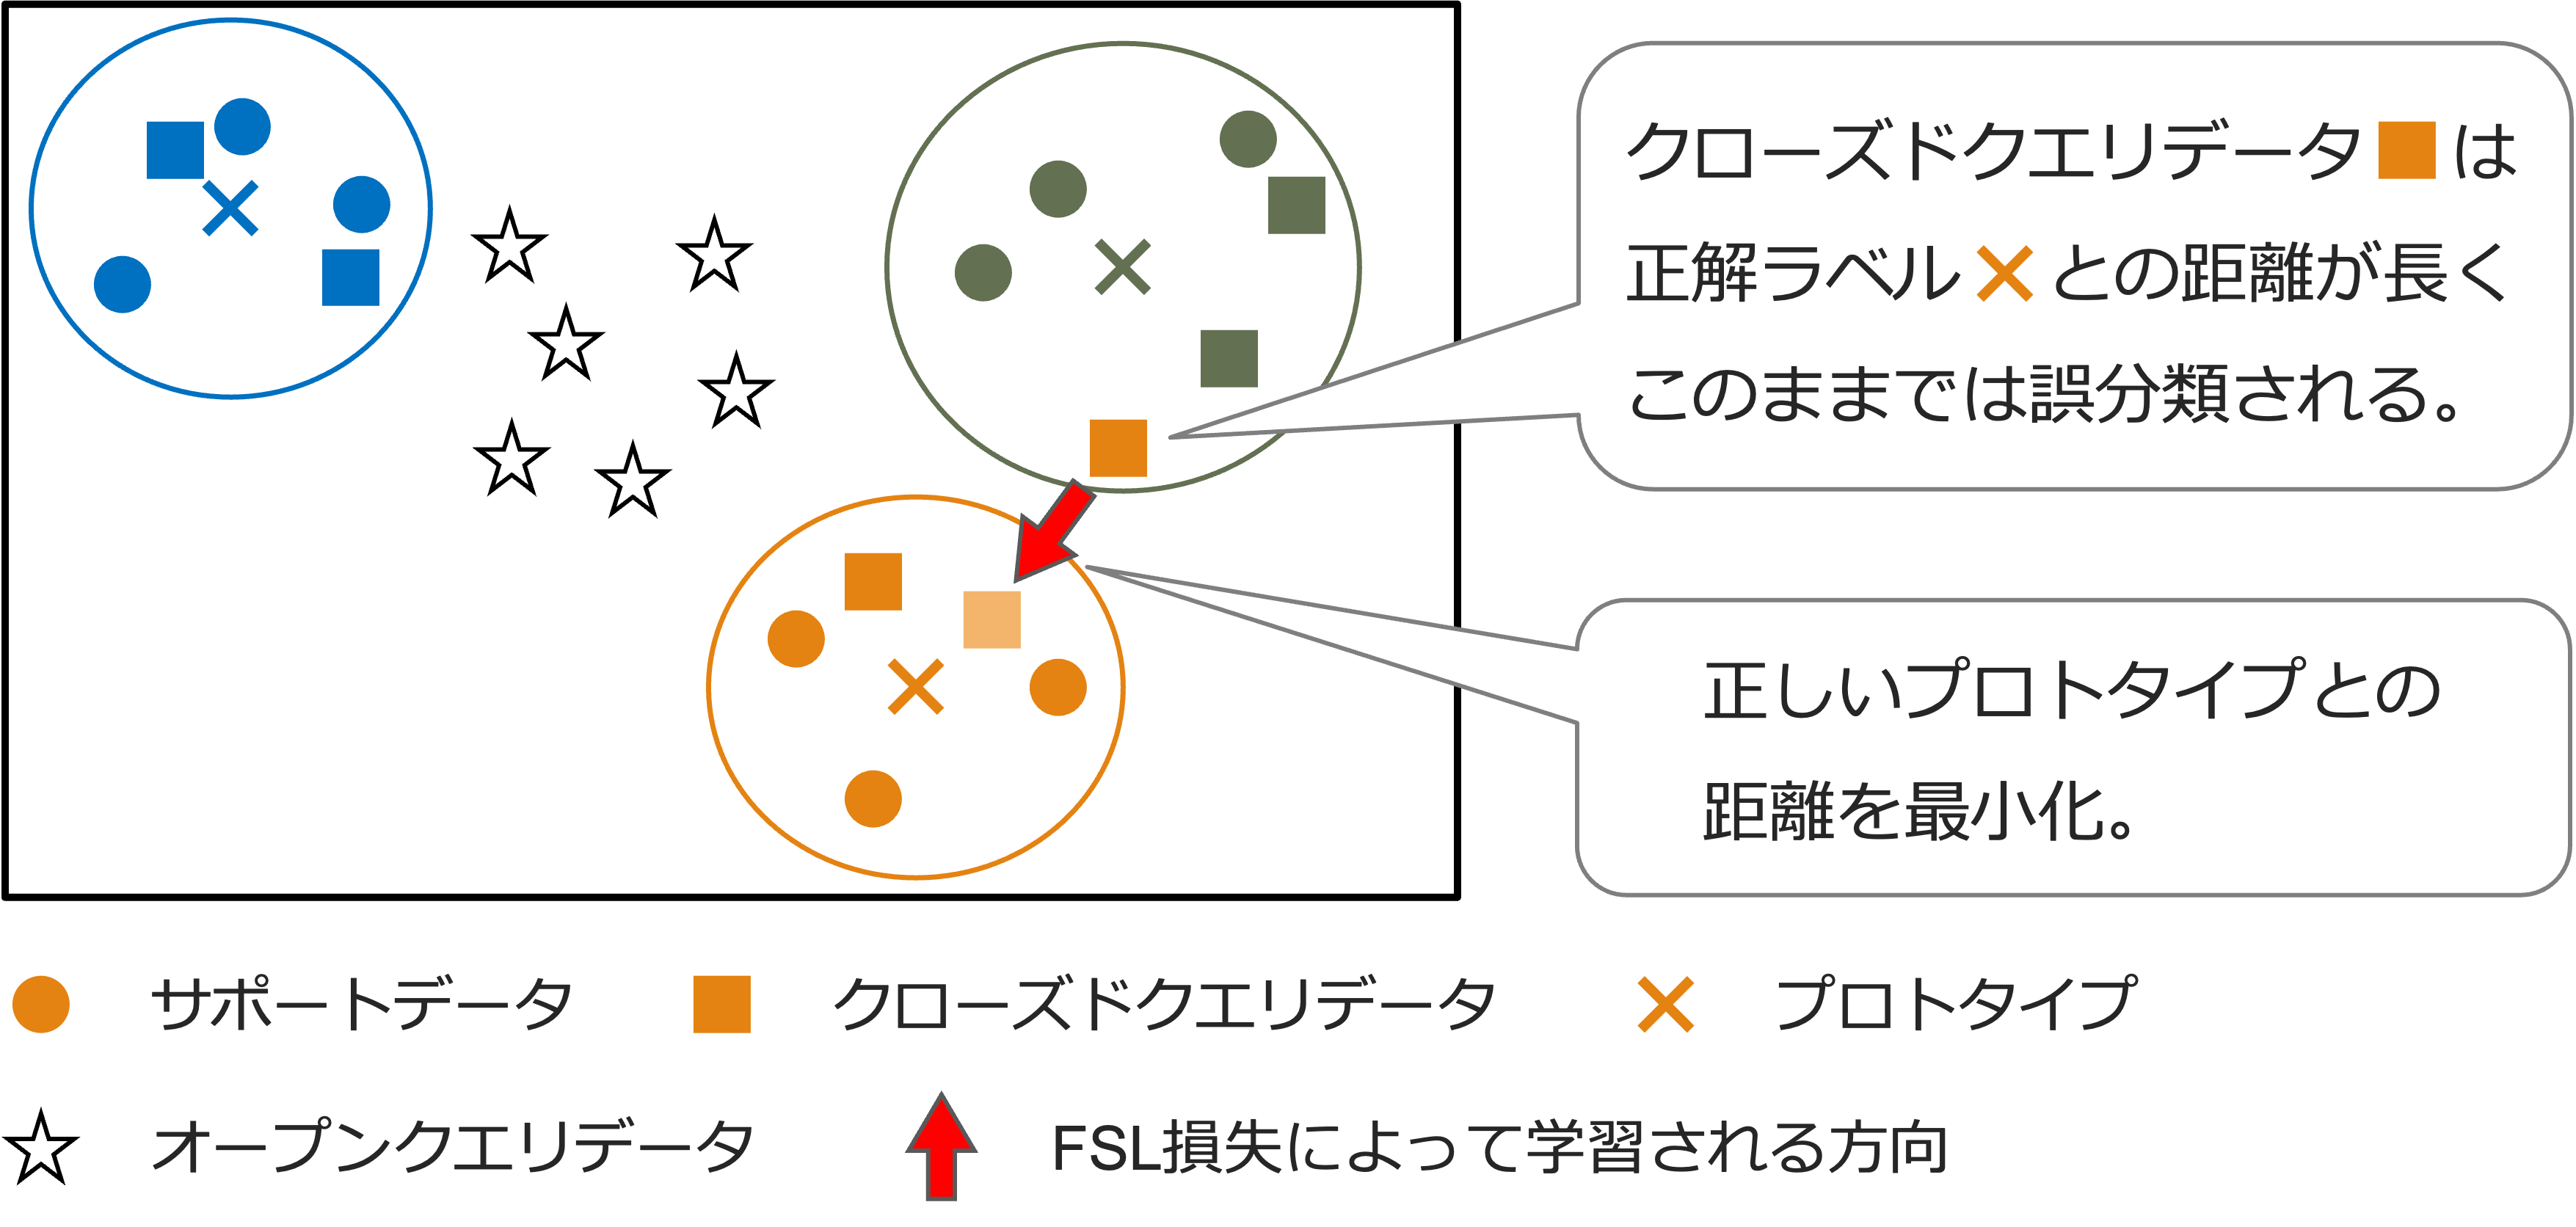
\includegraphics[width=\linewidth, keepaspectratio]{image/fsl_loss.png}
  \caption{FSL損失での学習が登録クラスの分類精度を向上させる例}
  \label{fig:fsl_loss}
\end{figure}
% 
以下に具体的なFSL損失の導出過程を述べる.

まず,プロトタイプとクローズドクエリデータの特徴ベクトル間のユークリッド距離を計算する.

\begin{equation}
  dist(f_{\phi}(\bm{x^C}),\mu_{k})=(f_{\phi}(\bm{x^C}) - \mu_{k})^{\top} (f_{\phi}(\bm{x^C}) - \mu_{k})
\end{equation}

\noindent
ここで,$f_{\phi}(\bm{x^C}) \in \mathcal{F}$ はクローズドクエリセットにおける入力画像 $\bm{x}^C \in \mathcal{X}^C$ の特徴ベクトルを表す.
ただし,$\mathcal{X} \subseteq \mathbb{R}^D$ は$D$次元の入力画像空間, $\mathcal{F} \subseteq \mathbb{R}^V$ は$V$次元の特徴空間を表す.
また,$f_{\phi}: \mathcal{X} \rightarrow \mathcal{F}$ はニューラルネットワークによる特徴抽出器であり,$\phi$ は学習可能なパラメータである.
$\mu_{k}$ は$k$番目のクラスのプロトタイプを表し,以下の式で算出される.

\begin{equation}
  \mu_{k} = \frac{1}{K} \sum_{\bm{x}^S_i \in \mathcal{X}^S_k} {f_\phi(\bm{x}^S_i)}
\end{equation}

\noindent
ここで,$\mathcal{X}^S_k$はクラス$k$におけるサポートデータ集合である.

次に,ユークリッド距離に負の符号を付けてソフトマックス関数に適用する.

\begin{equation}
\label{eq:fsl_prob}
  p_{\phi}(y^C=k \mid \bm{x}^C, \mathrm{M}) 
              = \frac{\exp(-dist(f_\phi(\bm{x}^C),\mu_{k}))}{\sum_{i \in \mathcal{Y}^S} {\exp(-dist(f_\phi(\bm{x}^C),\mu_{i}))}}
\end{equation}

\noindent
ここで,$p_{\phi}(\cdot \mid \cdot, \cdot)$は分類確率を表し,$\mathrm{M} = \left\{\mu_0, \mu_1, \ldots, \mu_{N-1} \right\}$はプロトタイプ集合を示す.
式 \ref{eq:fsl_prob}より,サポートデータとクローズドクエリデータの特徴ベクトル間のユークリッド距離が短いほど,正しく分類できる確率が高くなることが分かる.
よって,深層学習モデルの学習において,プロトタイプとクローズドクエリデータ間の距離が長い場合に大きな損失を与えることが望ましい.
最終的に,FSL損失はクロスエントロピー損失を用いて以下のように計算される.

\begin{equation}
  \mathcal{L}_{\mathrm{FSL}} [y^C, \bm{x}^C] = \sum_{(\bm{x}^C_i,y^C_i) \in \mathcal{D}^C} - \log {p_{\phi} (y^C_i \mid \bm{x}^C_i, \mathrm{M})}
\end{equation}

次に,OSR損失の計算の際は,学習用データセットから選択されるサポートセットとオープンクエリセットが用いられる.
ここで用いるサポートセットとは,前述したFSL損失の計算時に利用したものと同一のサンプルセットである.
一方,オープンクエリセットは,未登録クラスの検出能力を評価するためのサンプルセットであり,学習用データセットからサポートセットと異なるクラスの画像がランダムに選択される.

メタ学習の過程において,オープンクエリデータから抽出された特徴ベクトルを全てのプロトタイプから遠ざけることにより,
深層学習モデルは正確な未登録の検出能力を習得することが期待される.
図 \ref{fig:osr_loss}に,OSR損失で学習することにより効果的に未登録クラスの検出が可能になる例を示す.
% 
\begin{figure}[tbp]
  \centering
  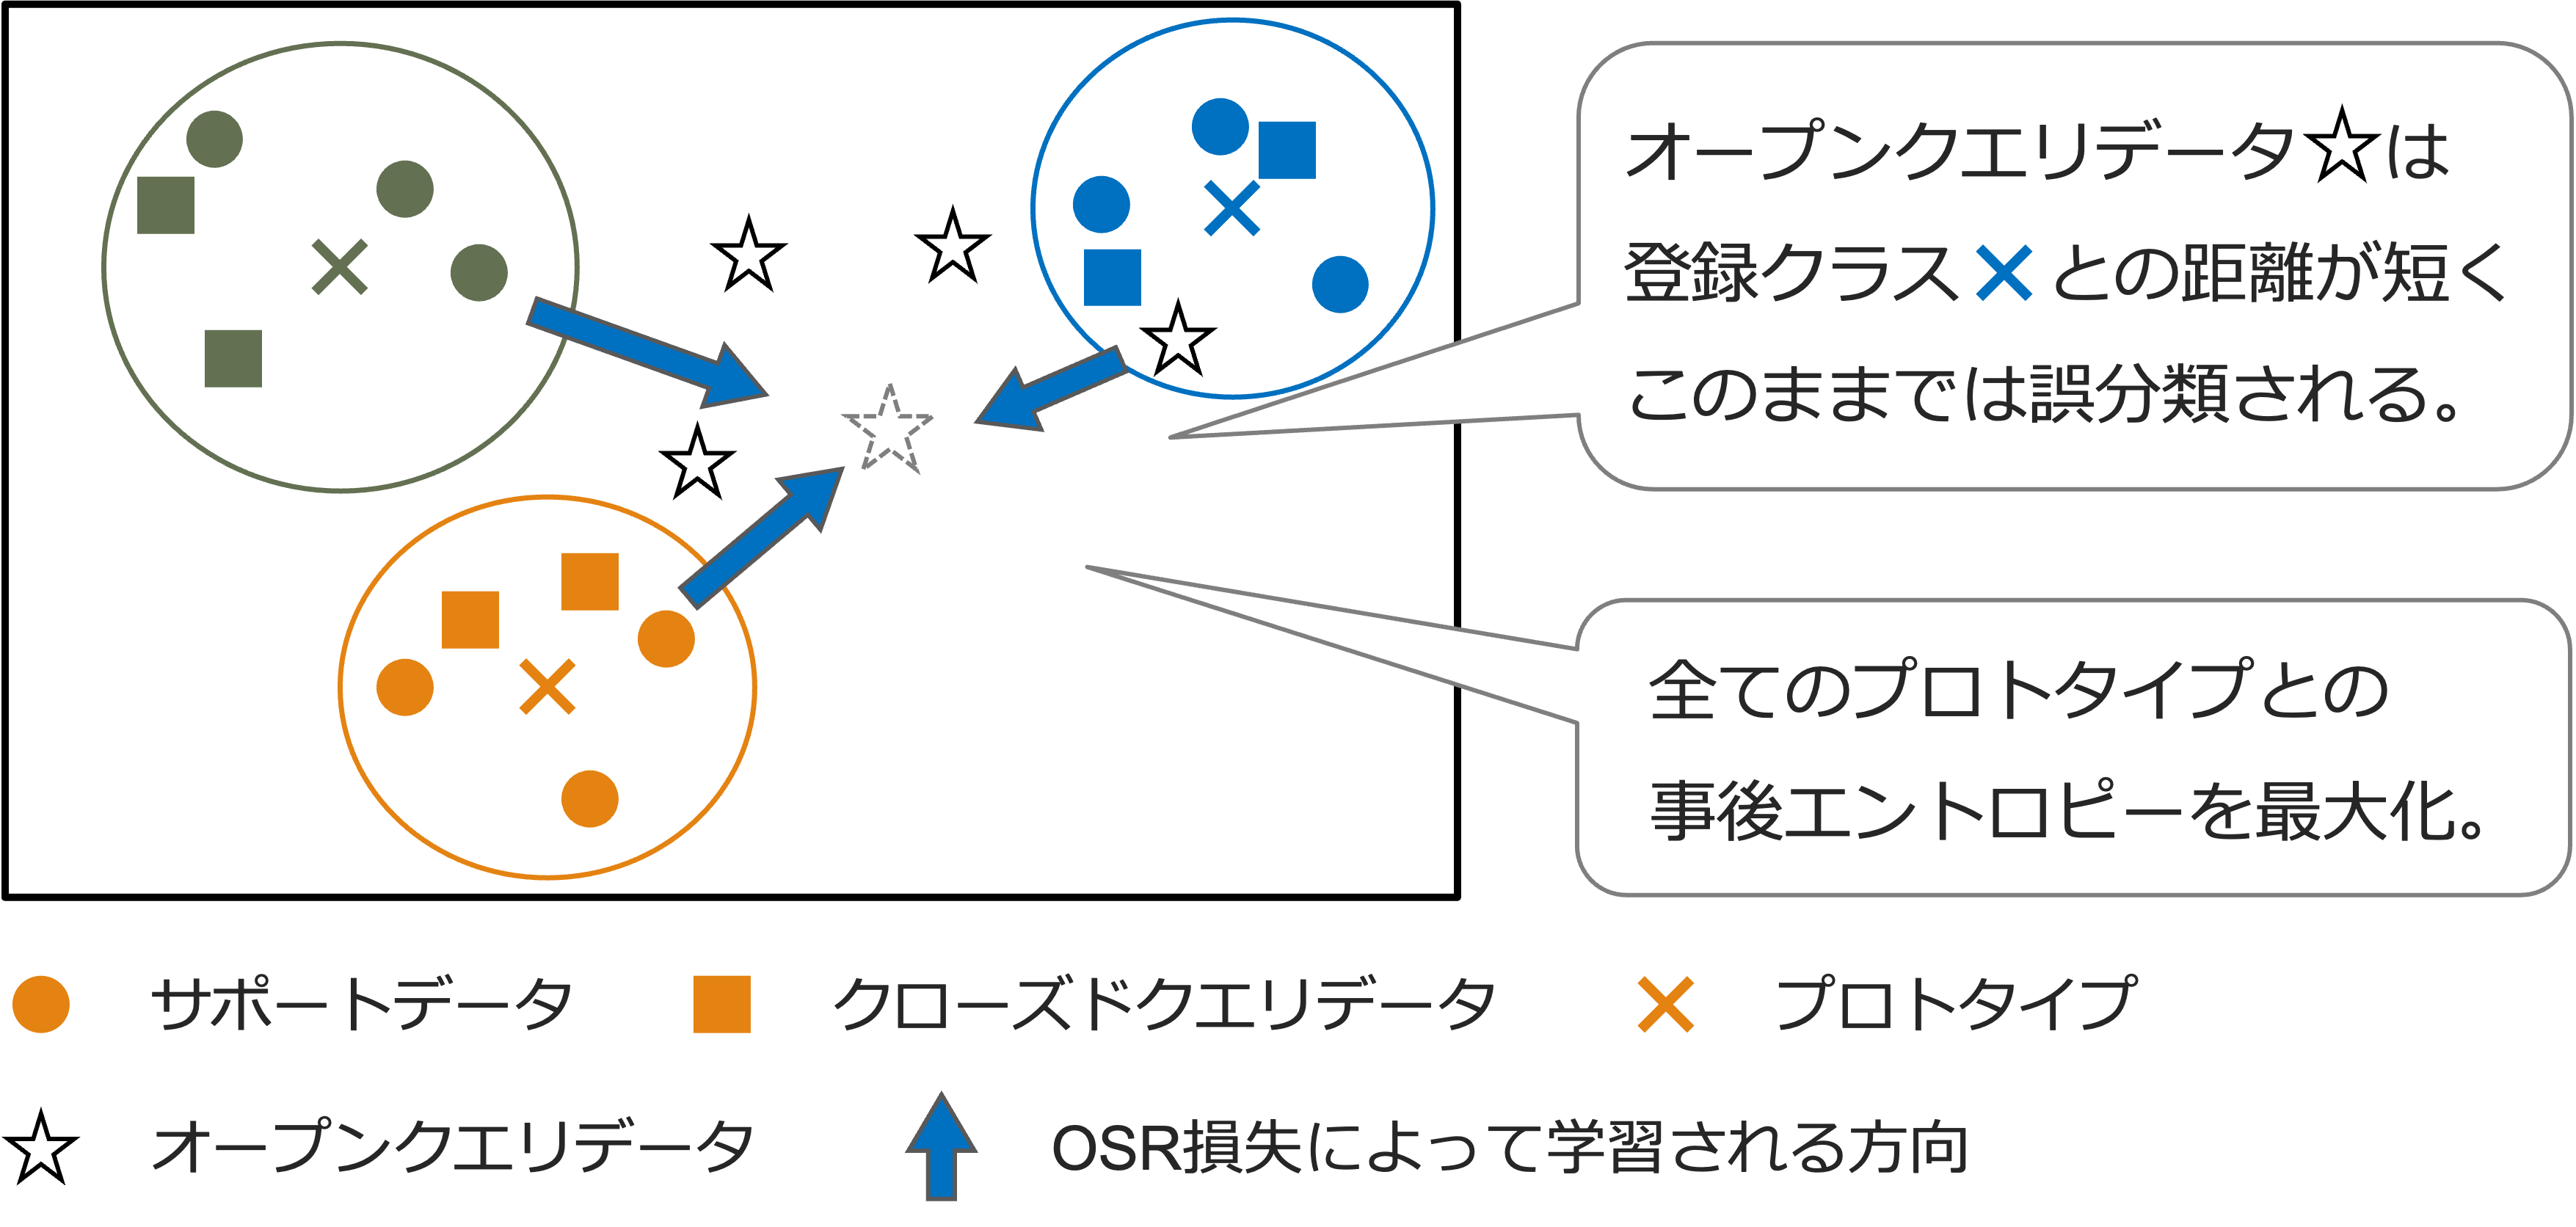
\includegraphics[width=\linewidth, keepaspectratio]{image/osr_loss.png}
  \caption{OSR損失での学習が未登録クラスの検出精度を向上させる例}
  \label{fig:osr_loss}
\end{figure}
% 
以下に具体的なOSR損失の導出過程を述べる.

モデルは,正しく未登録の検出を行うために,未登録クラスからのサンプルに遭遇した際,サポートデータのどのクラスにおいても大きな確率を割り当てるべきではない.
この場合,プロトタイプ集合に対するオープンクエリセットの最大のクラス確率$\underset{k \in \mathcal{Y}^S}{\max} {p_{\phi}(k|\bm{x}^O, \mathrm{M})}$が小さければ,未登録クラスのサンプルを適切に棄却することができる.
この目的を達成するため,PEELERアルゴリズムでは,オープンクエリセットのサンプルに対して,登録済みクラスへの分類確率の最小化を図る.
これは,オープンクエリデータの事後エントロピーを最大化すること,すなわち負のエントロピーを用いることで実現可能である.
この最適化を実現するための損失関数として,OSR損失は以下のように計算される.

\begin{equation}
    \mathcal{L}_{\mathrm{OSR}}[\bm{x}^O]
                = \sum_{k \in \mathcal{Y}^S} {p_{\phi}(k \mid \bm{x}^O, \mathrm{M}) \log{p_{\phi}(k \mid \bm{x}^O, \mathrm{M})}}
\end{equation}

最後に,分類損失の導出では,タスク$j$データセットから任意の数の画像枚数がベースデータとして選択される.
ベースデータは$\mathcal{D}^B = \left\{ \bm{x}^B_i \in \mathcal{X}^B, y^B_i \in \mathcal{Y}^B \right\}^{I J}_{i=1}$と表される.
ここで,$\bm{x}^B_i$はベースデータの入力画像空間$\mathcal{X}^B$における入力画像であり,$y^B_i$は教師ラベル空間$\mathcal{Y}^B$における教師ラベルを示す.
また,$I$はベースデータのクラス数,$J$は各クラスのサンプル数を表す.
% ここで,$\mathcal{X}^B$,$\mathcal{Y}^B$はそれぞれベースデータにおける入力画像空間,教師ラベル空間であり,
% $I$,$J$はそれぞれベースデータのクラス数,下クラスのサンプル数を示す.
この分類損失は,モデルが新しいドメインにおける分類タスクに対して,一般的かつ有用な特徴抽出を学習するために使用される.
モデルは,ベースデータから特徴抽出を行う際は特徴空間上での距離による分類ではなく,分類ヘッドを用いて学習を進める.
これは,学習用データセットに含まれる全てのクラスの分類問題を解くことと同義である.
分類確率の計算は,以下のソフトマックス関数を用いて行われる.

\begin{equation}
    p(y^B=k \mid \bm{x}^B;\phi,\mathbf{w}_k) 
        = \frac{\exp(\mathbf{w}_k^{\top} f_{\phi}(\bm{x}^B))}{\sum_{i \in \mathcal{Y}^B} \exp(\mathbf{w}_{i}^{\top} f_{\phi}(\bm{x}^B))}
\end{equation}

\noindent
ここで,$\mathbf{w}_k$は特徴抽出器の重みベクトルを表す.
よって,分類損失はクロスエントロピー損失を用いて以下のように表される.

\begin{equation}
  \mathcal{L}_{\mathrm{base}} [y^B, \bm{x}^B] = \sum_{(\bm{x}^B_i,y^B_i) \in \mathcal{D}^B} - \log {p(y^B_i \mid \bm{x}^B_i)}
\end{equation}

最終的に,FSL損失,OSR損失及び分類損失を線型結合し,バックプロパゲーションすることによりモデルのパラメータを更新する.
この学習手法により,深層学習モデルは登録クラスの正確な分類と未登録クラスの検出の両方を効果的に実現することが可能となる.
具体的には以下の最適化問題を解くことにより,$e \in \{1, 2, \ldots, N_e\}$エピソードにおけるモデル$h^*$を更新する.

\begin{align}
  h^* & = \arg \min_h \left\{ \sum_{(x_i,y_i) \in \mathcal{D}^C|y_i \in \mathcal{Y}^S}{\mathcal{L}_{\mathrm{FSL}}[y_i,h'(x_i)]} \right. \nonumber \\
      & \hspace{20mm} + \lambda \sum_{(x_i,y_i) \in \mathcal{D}^O|y_i \in \mathcal{Y}^O}{\mathcal{L}_{\mathrm{OSR}}[h'(x_i)]}
        \left. + \sigma \sum_{(x_i,y_i) \in \mathcal{D}^B|y_i \in \mathcal{Y}^B}{\mathcal{L}_{\mathrm{base}}[y^B_i,x^B_i]} \right\}
\end{align}

\noindent
ここで,$h'$は$e$エピソードにおいてサポートセットが登録されたモデルであり,
学習アルゴリズム$\mathcal{M}(\cdot)$,$e-1$エピソードにおけるモデル$h$を用いて以下のように表される.

\begin{align}
  h' = \mathcal{M}(h, D^S)
\end{align}

本研究では,FSOSRに用いられるメタ学習手法の1つであるPEELERを\ref{sec:ifor}節で提案したIFORに適用し,その有効性を検証する.
FSOSRと比較して,IFORはターゲットタスクが赤外線画像であることや,学習時と評価時に異なるデータセットを使用しているためドメインシフトが存在するなど,より厳しい問題設定となっている.
したがって,これらの本質的に異なる問題設定に対して,メタ学習アプローチの汎用性と頑健性を実証的に評価する.

\section{未登録クラスに対する多クラス分類の高精度化に向けたクラスタリングに基づく損失関数}

\subsection{メタ学習にクラスタリングを導入する目的}
\label{subsec:purpose}

既存のOSRやFSOSRは,未登録クラスの検出に取り組んでおり,多クラス分類に適した特徴空間の構築が十分に行われていなかった.
図 \ref{fig:classification_goals}に未登録クラスの多クラス分類の概要を示す.
% 
\begin{figure}[tbp]
  \centering
  \begin{subfigure}[b]{0.45\linewidth}
    \centering
    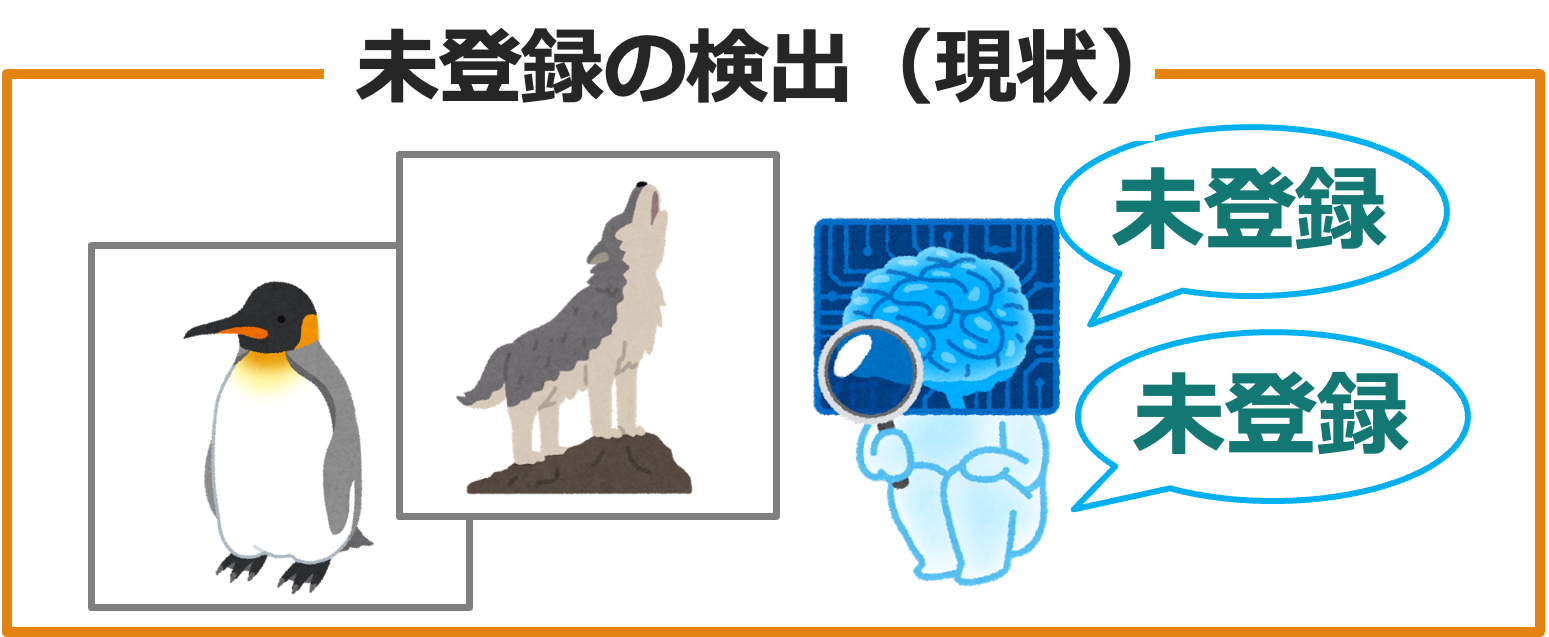
\includegraphics[width=\linewidth, keepaspectratio]{image/detection.png}
    \caption{未登録クラスの検出}
    \label{fig:detection}
  \end{subfigure}
  \hfill
  \begin{subfigure}[b]{0.45\linewidth}
    \centering
    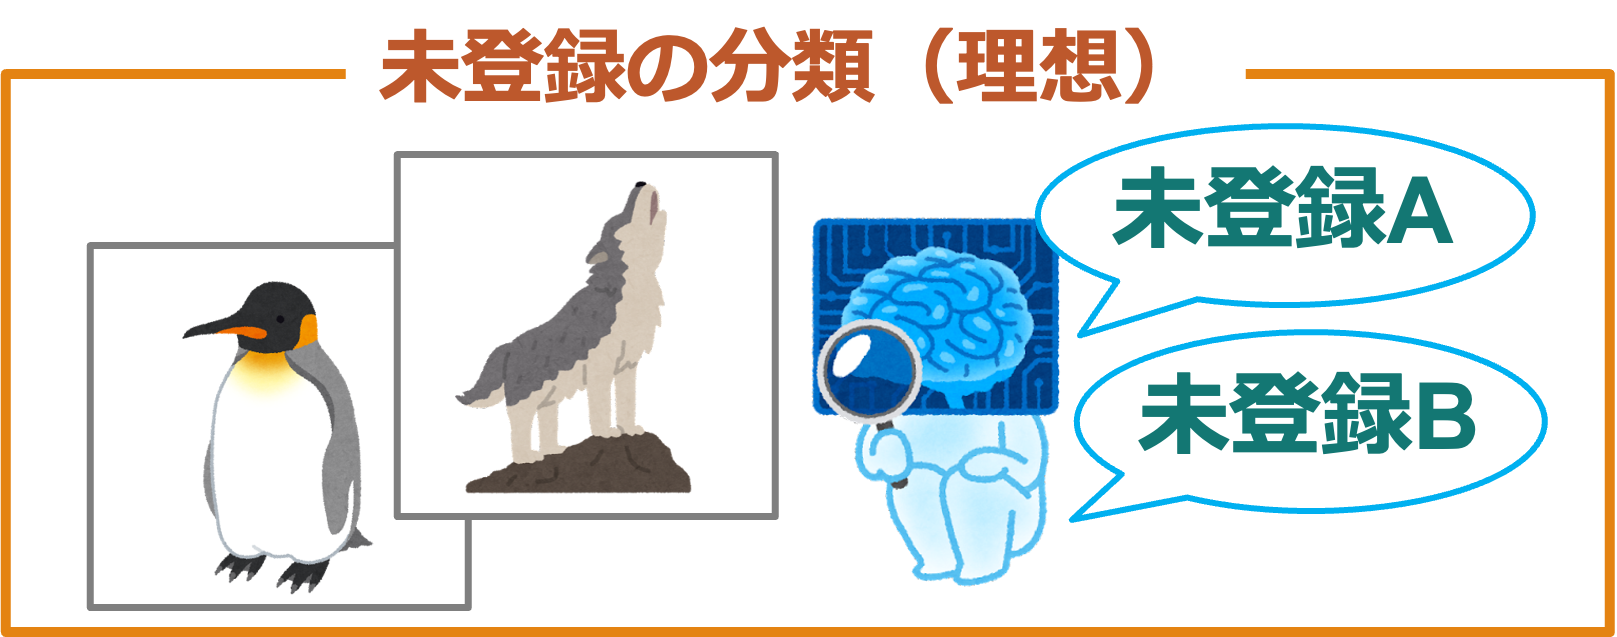
\includegraphics[width=\linewidth, keepaspectratio]{image/classification.png}
    \caption{未登録クラスの分類}
    \label{fig:classification}
  \end{subfigure}
  \caption{未登録クラスの多クラス分類}
  \label{fig:classification_goals}
\end{figure}
%
\ref{sec:detection_approach}節では,既存手法と同様に図 \ref{fig:detection}のような未登録クラスの検出に取り組んでいた.
これに対し本説ではIFORを発展させ,図 \ref{fig:classification}のような未登録クラスに対する多クラス分類精度の向上に焦点を当てている.
図 \ref{fig:feature_space}は,学習時における特徴空間上の各クラス分布を示す2つの例である.
% 
\begin{figure}[tbp]
  \centering
  \begin{subfigure}[b]{0.45\linewidth}
    \centering
    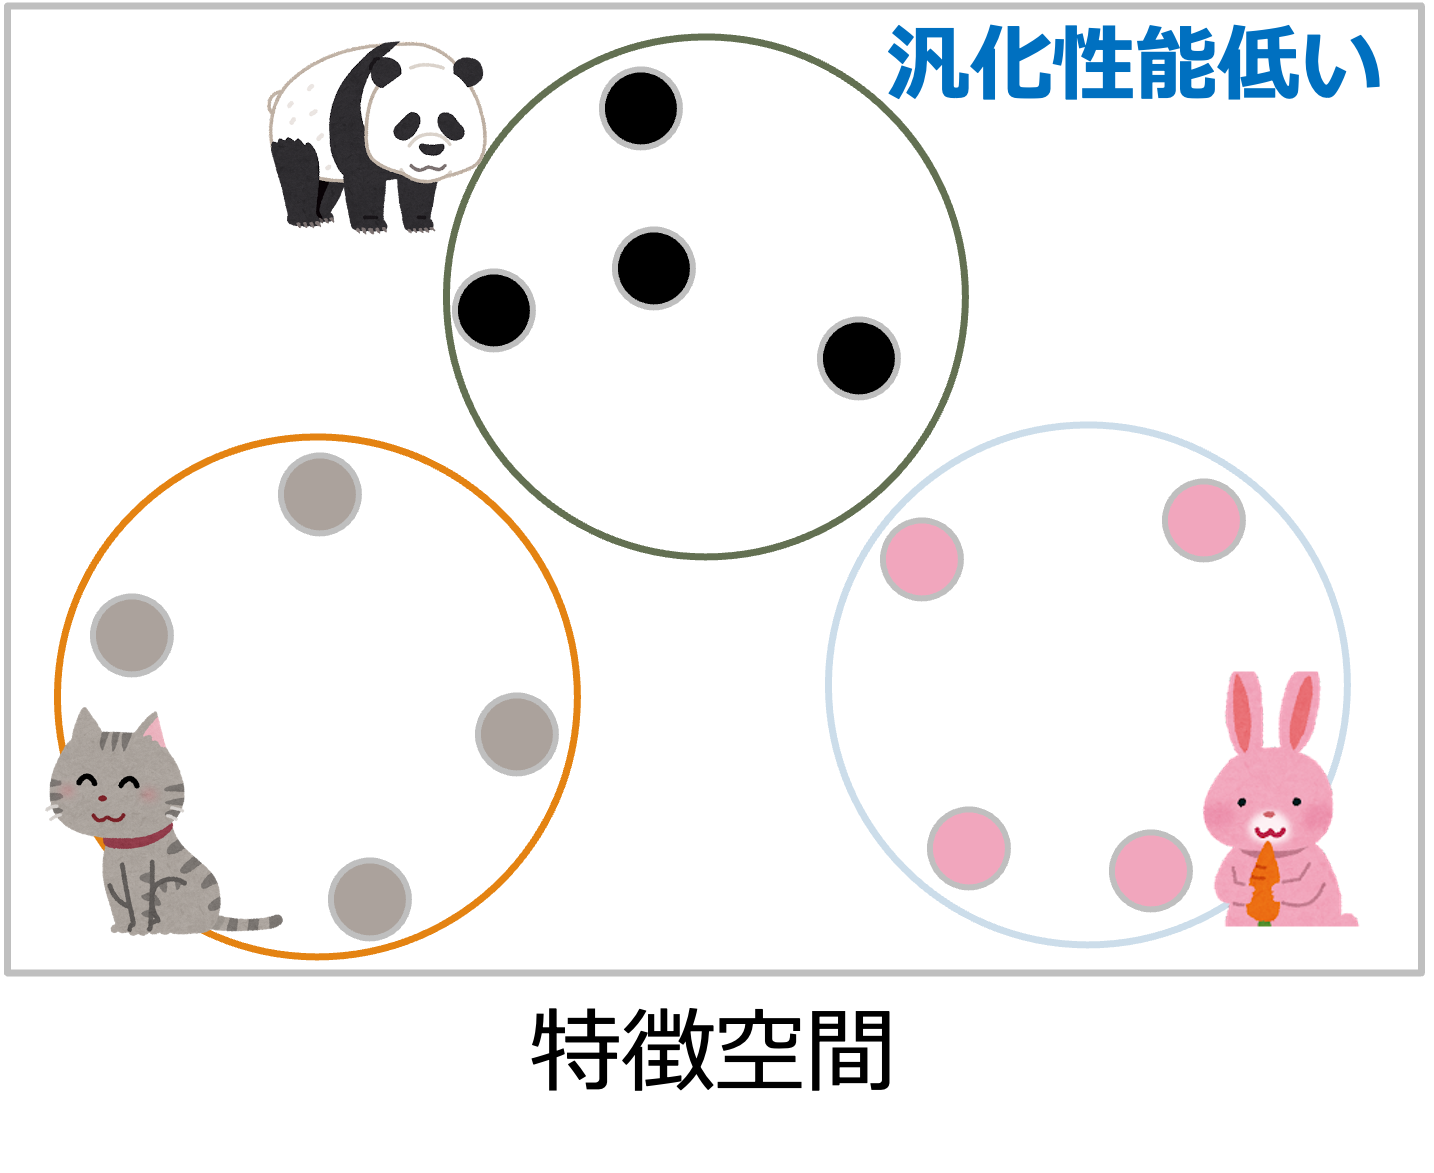
\includegraphics[height=0.9\linewidth, keepaspectratio]{image/bad_featurespace.png}
    \caption{汎化性能の低い特徴空間の例}
    \label{fig:bad_featurespace}
  \end{subfigure}
  \hfill
  \begin{subfigure}[b]{0.45\linewidth}
    \centering
    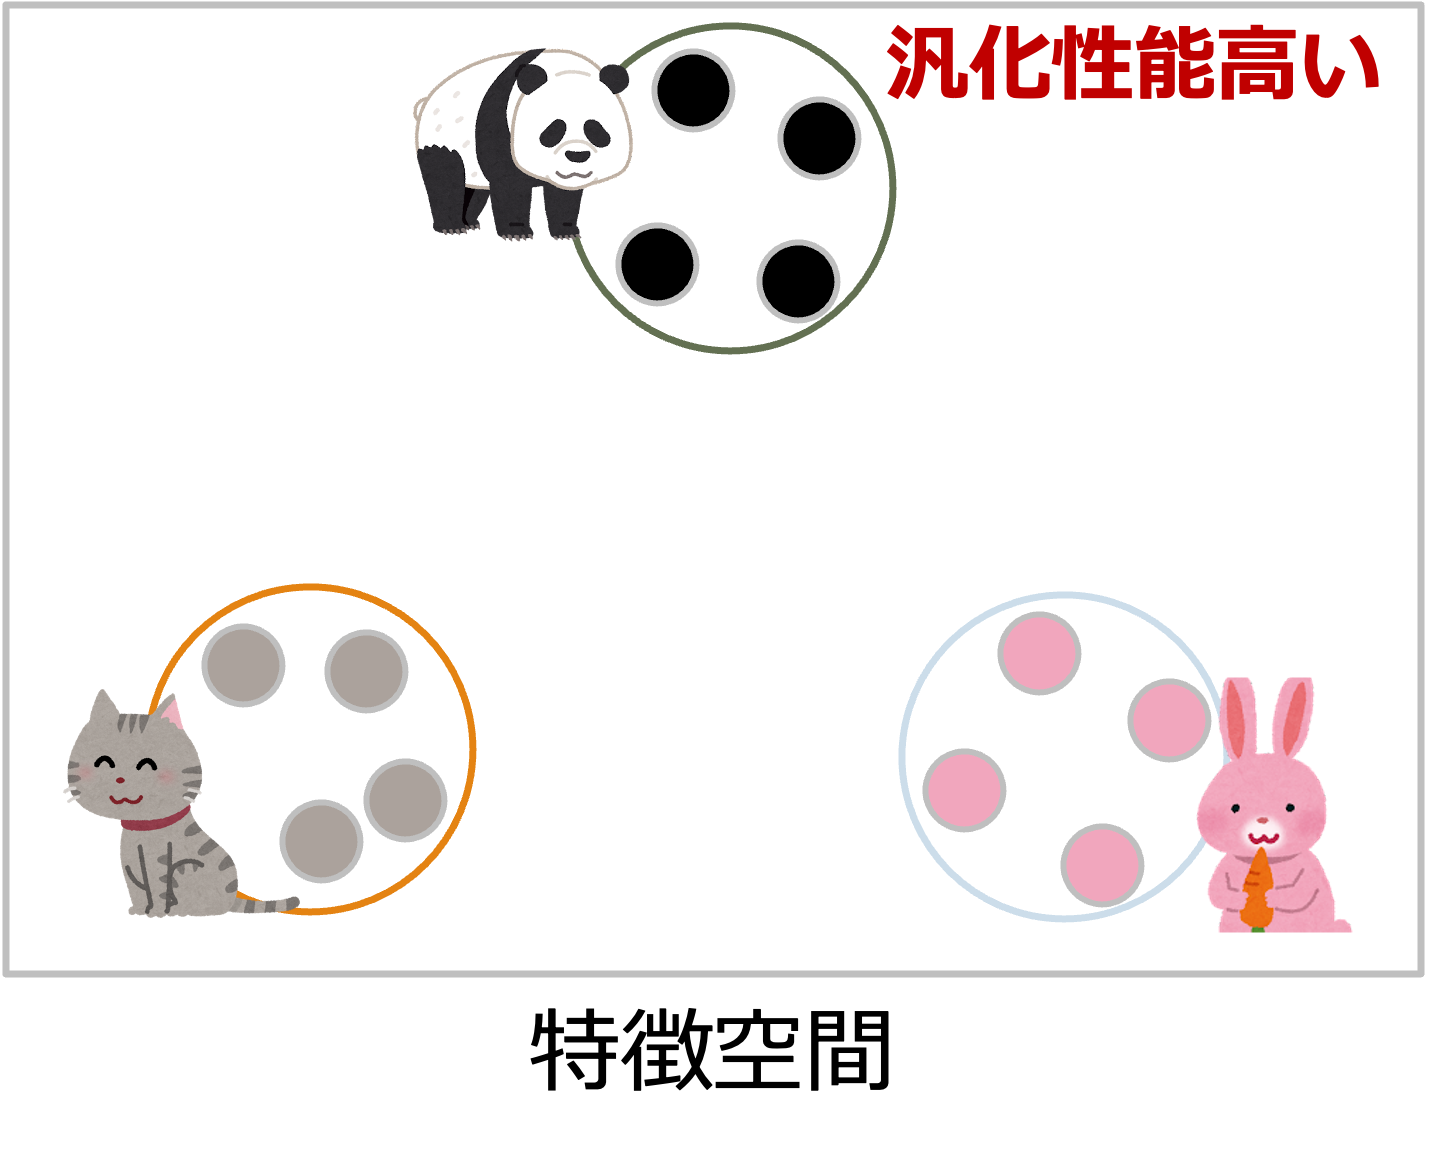
\includegraphics[height=0.9\linewidth, keepaspectratio]{image/good_featurespace.png}
    \caption{汎化性能の高い特徴空間の例}
    \label{fig:good_featurespace}
  \end{subfigure}
  \caption{学習時における特徴空間上の各クラス分布の例}
  \label{fig:feature_space}
\end{figure}
% 
四角形の枠線は特徴空間,点は特徴ベクトル,点を包含している丸い枠線はクラス分布領域の境界を表している.
図 \ref{fig:bad_featurespace}及び図 \ref{fig:good_featurespace}に示された特徴空間は,
いずれも登録済みのクラスに対して同程度の分類精度であるが,評価時のドメインシフトなどを考慮した場合,
図 \ref{fig:good_featurespace}の特徴空間の方が,新規地域に対する高い汎化性能を有していると考えられる.
これは,図 \ref{fig:good_featurespace}の方がクラス内分散が小さく,かつクラス間分散が大きいため,
新規地域においても分類が容易となるような特徴空間の構築が期待できるからである.

したがって,本研究では,メタ学習にクラスタリングに基づく損失関数を導入することにより,
クエリセットに対するクラス内分散の最小化・クラス間分散の最大化を実現する.
これにより,IFORにおける未登録クラスの多クラス化に向けて分類精度の向上を図る.

\subsection{損失関数}

本研究では,FSL損失,OSR損失,分類損失に加え,\ref{subsec:purpose}で述べたクラスタリングに基づく損失関数としてk-means損失と Between-Class損失 (BC損失)を導入する.
k-means損失は,Chinら \cite{k-means}が異常検知タスクにおいて提案した損失関数であり,k-meansクラスタリングによって集約される類似した性質を持つ特徴量から,
より識別的な特徴表現の学習を可能にする.
% より優れた特徴表現を学習するための損失関数である.
IFORフレームワークにおいて,k-means損失は以下のように定義される.

\begin{align}
\mathcal{L}_{\mathrm{k-means}} = \sum_i{\min_k \lVert f(x_i)-c_k \rVert_2}
\end{align}

\noindent
ここで,$f(x_i)$は$i$番目の入力画像を特徴抽出器$f(\cdot)$に入力した際の特徴量,$c_k$は$k$番目のクラスタ中心を表す.

k-means損失による学習の例を図 \ref{fig:kmeans_loss}に示す.
% 
\begin{figure}[tbp]
  \centering
  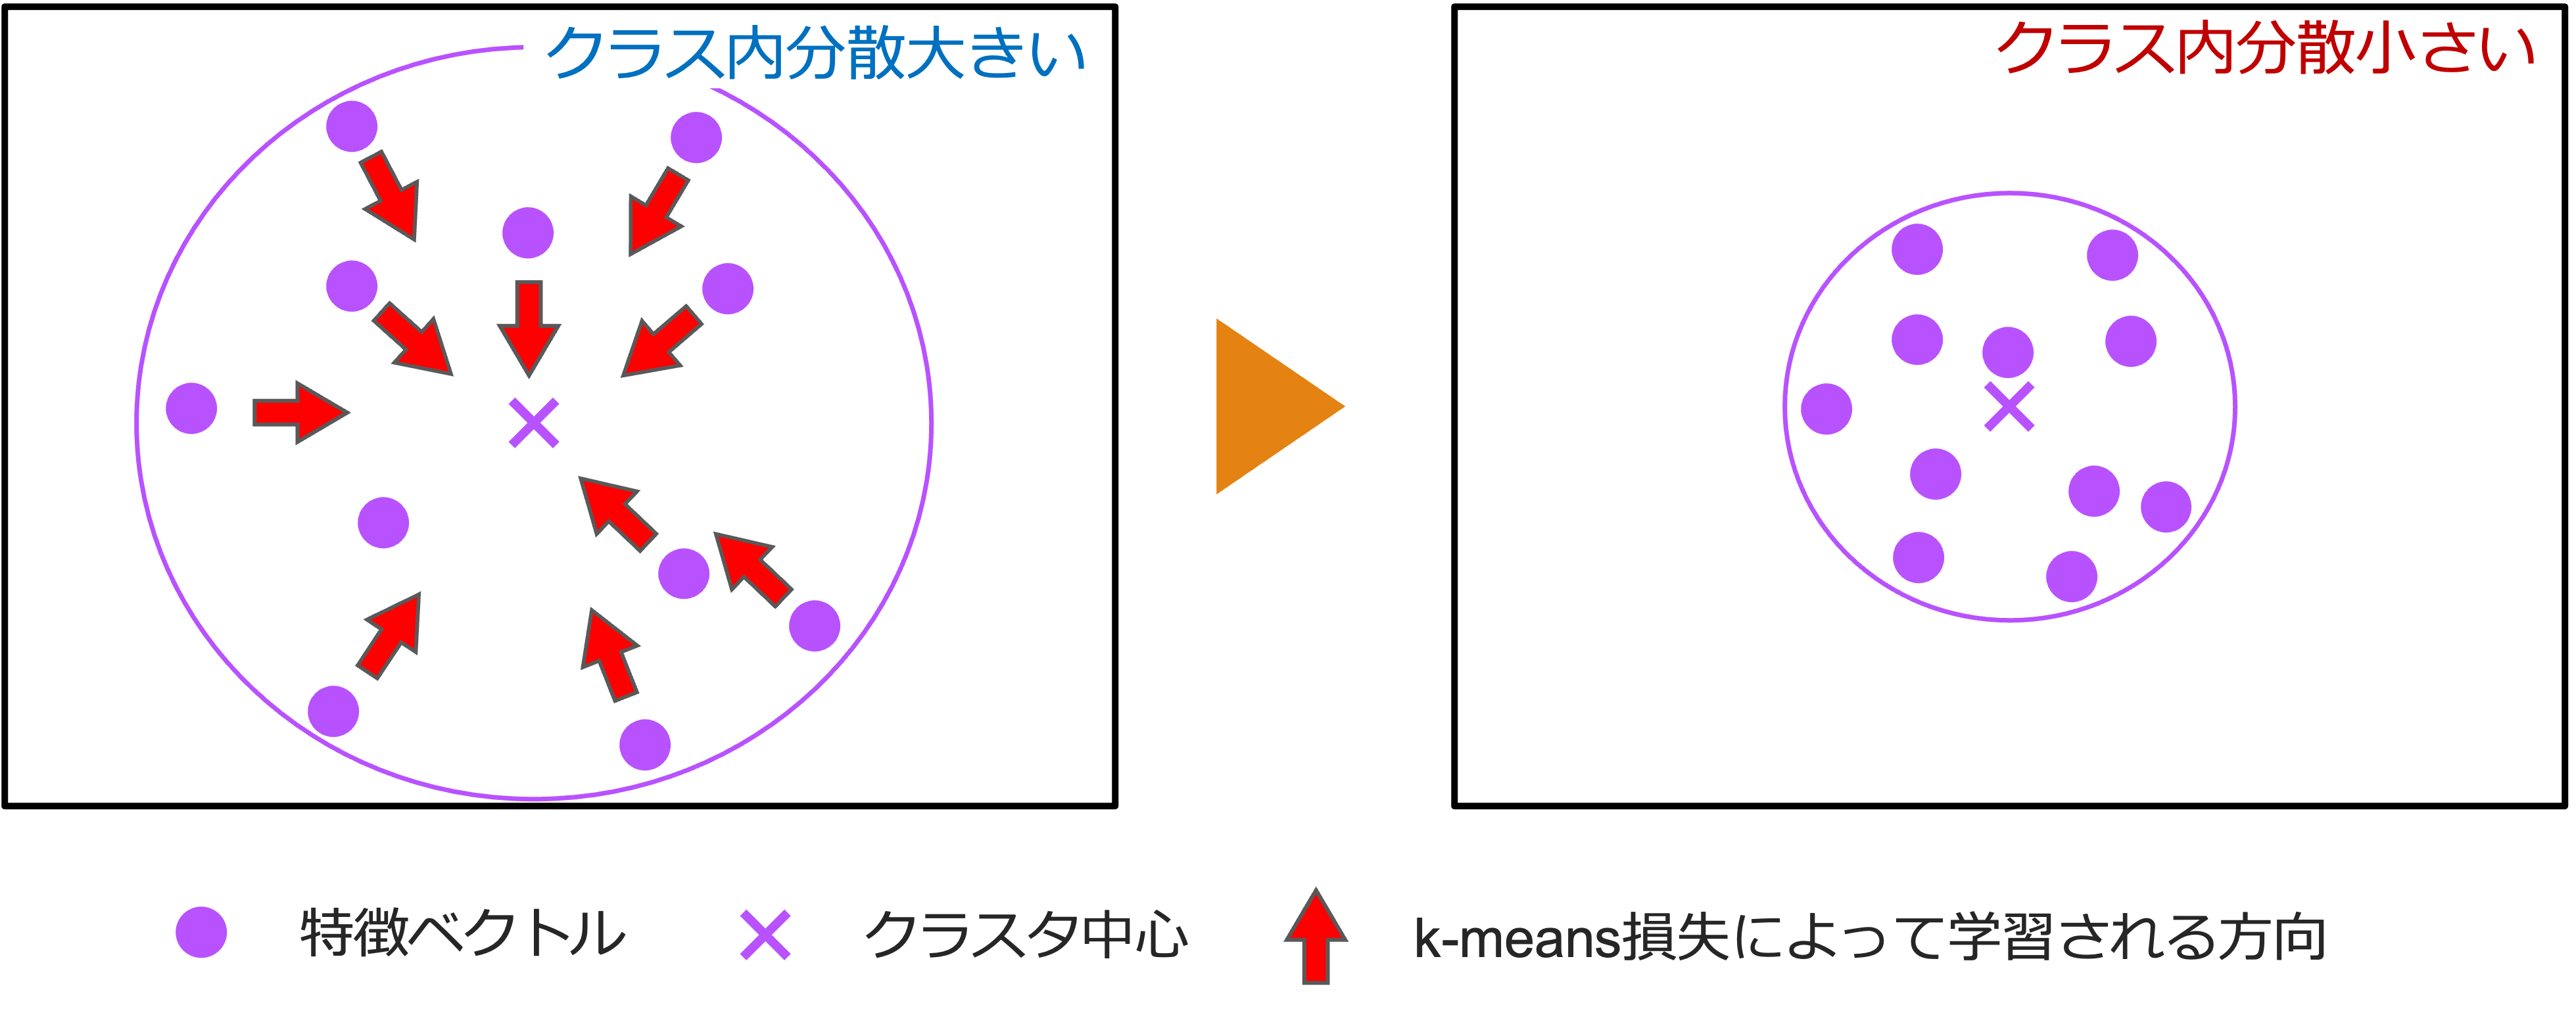
\includegraphics[width=\linewidth, keepaspectratio]{image/kmeans_loss.png}
  \caption{k-means損失によってクラス内分散が小さくなる例}
  \label{fig:kmeans_loss}
\end{figure}
% 
この損失関数の最小化により,各クラスタ中心とそのクラスタに属する特徴ベクトルとの距離が最小となることが期待される.
本研究では,類似した性質を持つ特徴量のクラスタリングにより,特徴空間上の各クラスのクラス内分散を最小化することを目指し,k-means損失の有効性を検証する.

一方,BC損失は,クラス分布のコンパクトな表現に加え,各クラスの分布が可能な限り離れているような特徴空間の構築が,
多クラス分類性能の向上に寄与するという考えに基づいている.
IFORフレームワークにおいて,BC損失は以下のように定義される.

\begin{align}
  \mathcal{L}_{\mathrm{Between-Class}} = -\log{\sum_{k_1} {\sum_{k_2} {\lVert c_{k_1} - c_{k_2} \rVert_2}}}
\end{align}

\noindent
ここで,$c_{k_1}$と$c_{k_2}$は$k_1$番目,$k_2$番目のクラスタ中心を表す.
負の符号を付与することにより,クラス間分散の最大化問題を損失関数の最小化問題として扱っている.

BC損失による学習の例を図 \ref{fig:bc_loss}に示す.
% 
\begin{figure}[tbp]
  \centering
  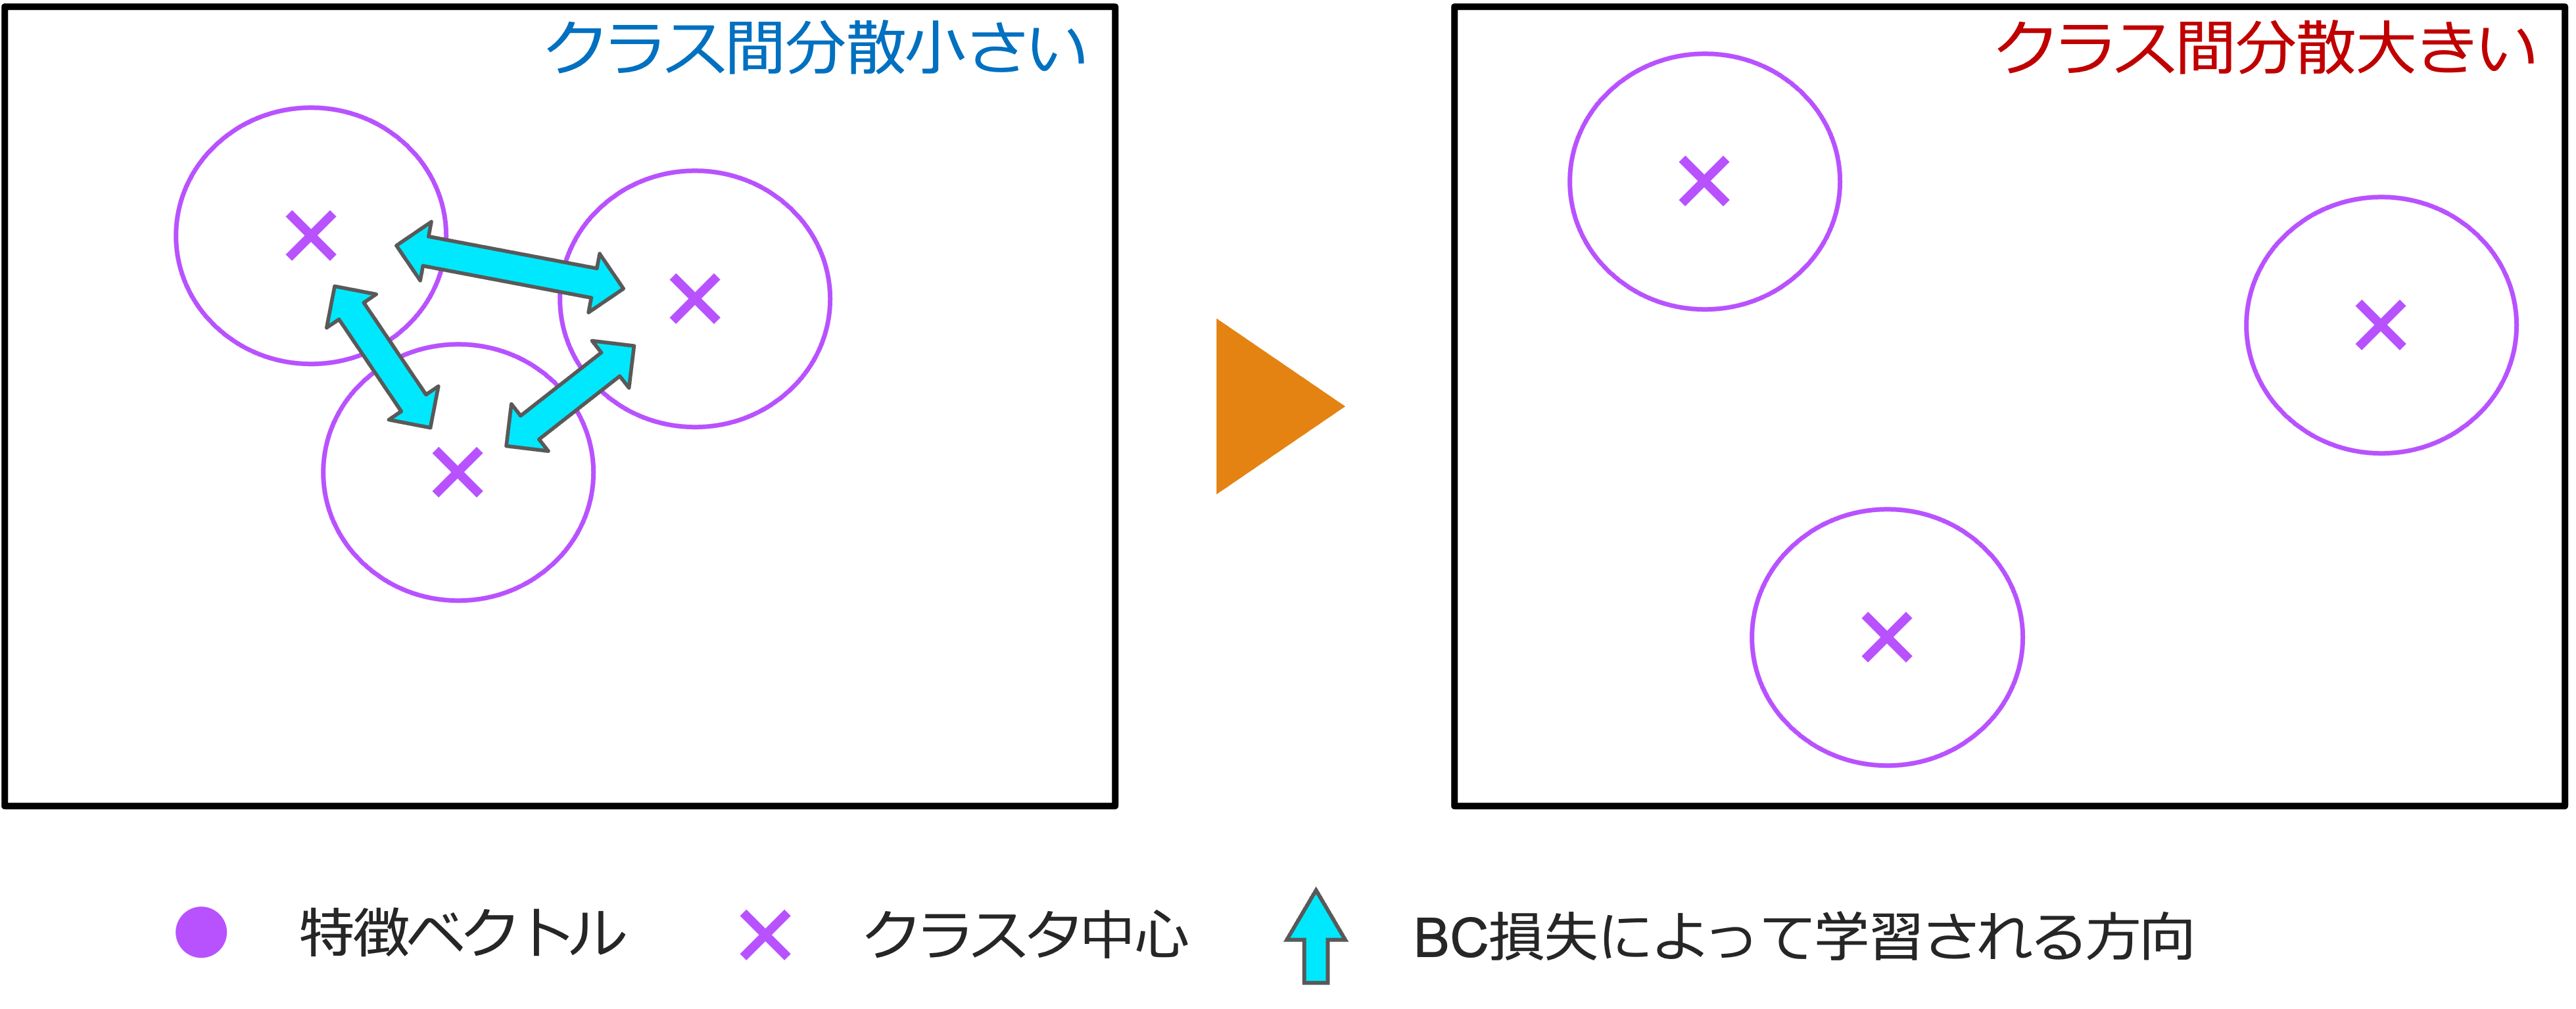
\includegraphics[width=\linewidth, keepaspectratio]{image/bc_loss.png}
  \caption{Between-Class損失によってクラス間分散が大きくなる例}
  \label{fig:bc_loss}
\end{figure}
%
この損失関数では,k-meansクラスタリングによって得られる各クラスタ中心間の距離を最大化することにより,クラス間分散の最大化を図っている.
% /01_draft/chapter4/chapter4_v2.tex

\chapter{評価実験}

\section{データセット}

IFOR手法の開発において,地域間のドメインシフトを考慮したモデルの性能評価は重要である.
このドメインシフトを実現するため,学習用と評価用のデータセットを異なる地域から選定した.
具体的には,学習用データセットとして南米の野生動物画像を集めたWCS Camera Traps (WCS) \cite{wcs}を,
評価用データセットとして北米の野生動物画像から構成されるCaltech Camera Traps (CCT) \cite{cct}をそれぞれ採用した.

本実験では,提案手法の有効性を多角的に検証するため,各データセットにおいて赤外線画像と可視光画像それぞれから構成される2種類のデータセットを作成した.
このアプローチにより,提案手法が赤外線画像特有の性質に対して有効であるのか,
あるいは,赤外線画像や可視光画像を問わず広義の画像分類に対して有効であるのかを検証することが可能となる.

データセットの前処理では,各画像を赤外線画像と可視光画像に分類し,
アノテーションとして提供されているバウンディングボックスに基づいてクロッピングを行い,動物が存在している領域を切り出した.
バウンディングボックスに基づき動物領域が切り出された例を図 \ref{fig:cropping}に示す.
% 
\begin{figure}[tbp]
  \centering
  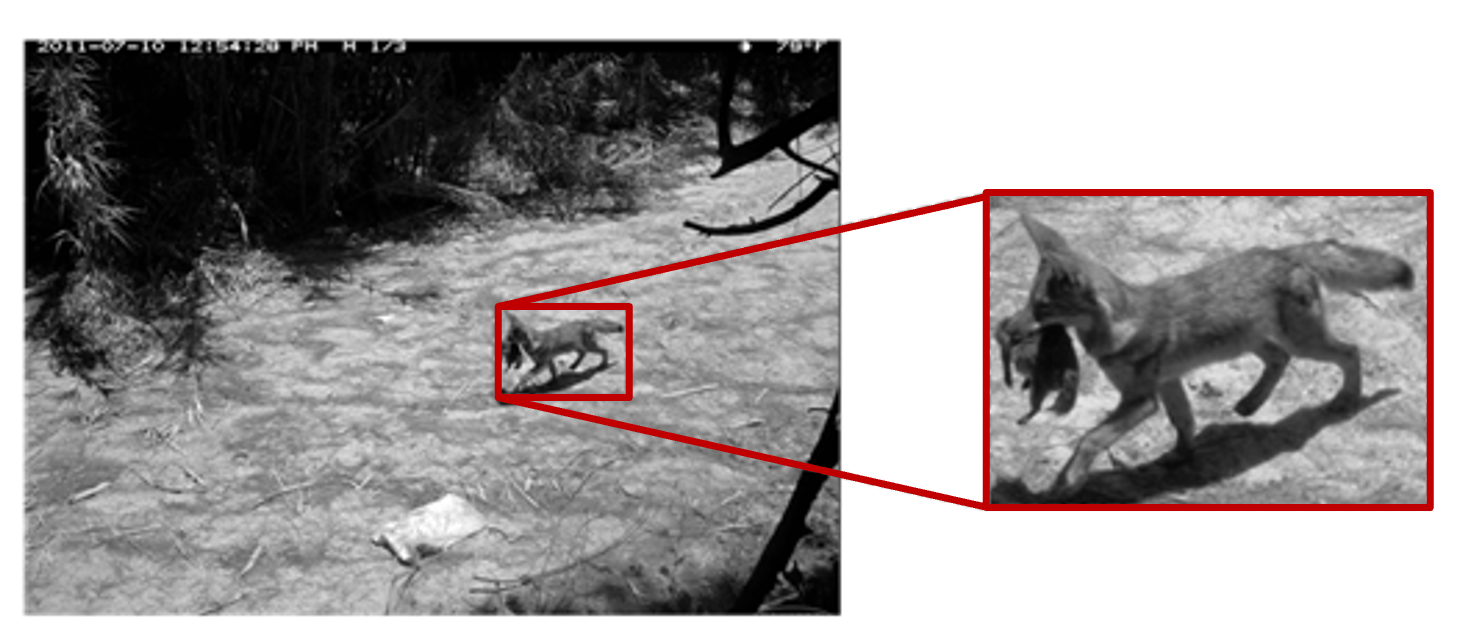
\includegraphics[width=\linewidth, keepaspectratio]{image/cropping.png}
  \caption{バウンディングボックスによって動物領域が切り出されている例}
  \label{fig:cropping}
\end{figure}
% \begin{figure}[tbp]
%   \centering
%   \begin{subfigure}[b]{0.45\linewidth}
%     \centering
%     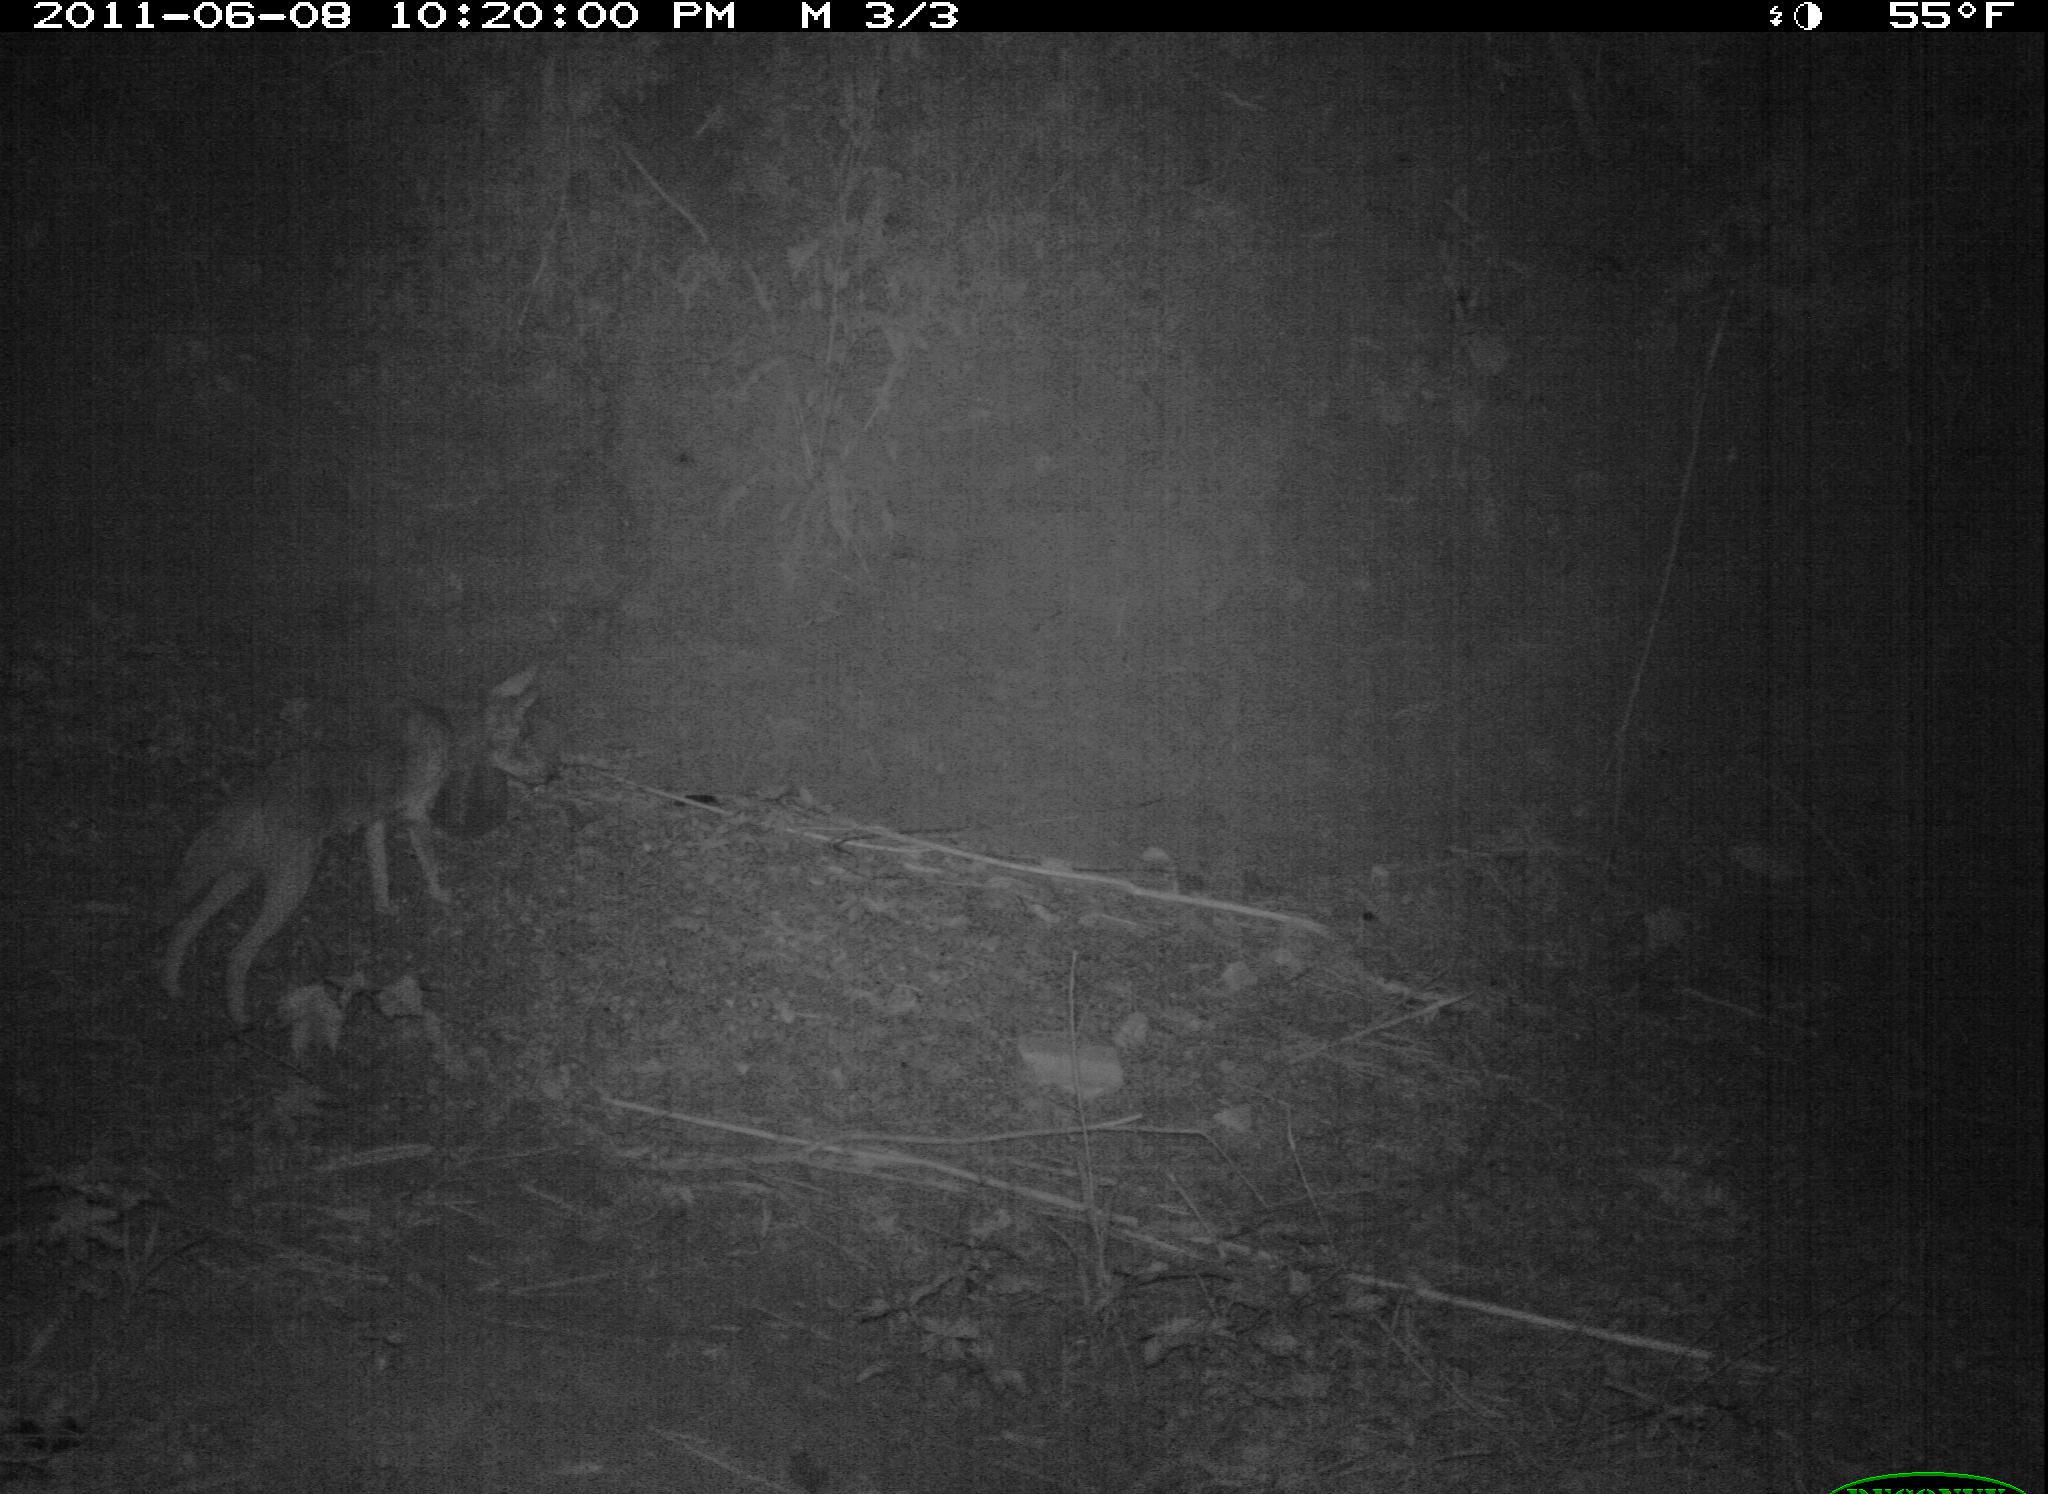
\includegraphics[height=0.9\linewidth, keepaspectratio]{image/coyote_full.png}
%     \caption{原画像}
%     \label{fig:fullimg}
%   \end{subfigure}
%   \hfill
%   \begin{subfigure}[b]{0.45\linewidth}
%     \centering
%     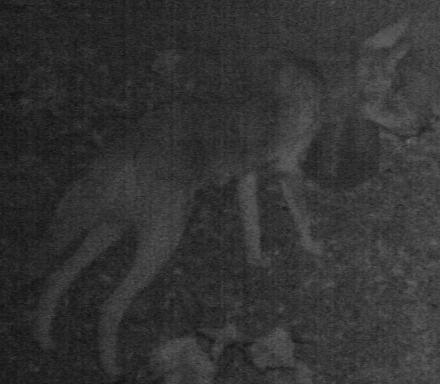
\includegraphics[height=0.9\linewidth, keepaspectratio]{image/coyote_cropped.png}
%     \caption{クロッピングされた画像}
%     \label{fig:croppedimg}
%   \end{subfigure}
%   \caption{バウンディングボックスによって}
%   \label{fig:cropbybbox}
% \end{figure}
% 
その後,実験の公平性を確保するため,赤外線画像と可視光画像による学習用データセット間でクラス数と画像枚数を同数に統一した.
同様に,評価用データセットについてもクラス数と画像枚数を同一に設定した.
具体的には,学習用データセットは28クラス,各クラス約500枚ずつの合計14,000枚の画像で構成され,
評価用データセットは11クラス,各クラス100枚ずつの合計1,100枚の画像により構成される.
これらの処理により,学習用データセットとして赤外線画像及び可視光画像による2種類の WCS データセット,
評価用データセットとして赤外線画像及び可視光画像による2種類の CCT データセットの計4種類のデータセットを作成した.
ただし,画像の前処理過程において,学習用データセットでは赤外線画像が13,687枚,可視光画像が13,812枚と若干の不均衡が生じたが,
この僅かな差異は実験結果に重大な影響を及ぼさないと考えられる.
これらの前処理によって作成された各データセットの詳細を表 \ref{tbl:wcs}及び表 \ref{tbl:cct}に示す.

\begin{table}[tbp]
  \centering
  \caption{学習用データセット (WCS Camera Traps)データセットの詳細}
  \label{tbl:wcs}
  \begin{tabular}{c|c|c}
      \hline
      動物種                    & 赤外線画像(枚) & 可視光画像(枚) \\ \hline\hline
      acryllium vulturinum     & 500          & 500          \\
      aepyceros melampus       & 500          & 500          \\
      bos taurus               & 500          & 500          \\
      capra aegagrus           & \textbf{337} & 500          \\
      cephalophus nigrifrons   & 500          & 500          \\
      crax rubra               & 500          & 500          \\
      cuniculus paca           & 500          & \textbf{495} \\
      dasyprocta punctata      & 500          & 500          \\
      equus quagga             & 500          & 500          \\
      giraffa camelopardalis   & 500          & 500          \\
      leopardus pardalis       & 500          & 500          \\
      loxodonta africana       & 500          & 500          \\
      madoqua guentheri        & 500          & 500          \\
      mazama americana         & 500          & 500          \\
      mazama temama            & 500          & 500          \\
      meleagris ocellata       & 500          & 500          \\
      mitu tuberosum           & 500          & 500          \\
      nasua narica             & \textbf{350} & 500          \\
      panthera onca            & 500          & 500          \\
      papio anubis             & 500          & 500          \\
      pecari tajacu            & 500          & 500          \\
      phacochoerus africanus   & 500          & \textbf{317} \\
      psophia leucoptera       & 500          & 500          \\
      puma concolor            & 500          & 500          \\
      syncerus caffer          & 500          & 500          \\
      tapirus terrestris       & 500          & 500          \\
      tayassu pecari           & 500          & 500          \\
      urocyon cinereoargenteus & 500          & 500          \\ \hline\hline
      合計                      & 13,687       & 13,812       \\ \hline
  \end{tabular}
\end{table}

\begin{table}[tbp]
  \centering
  \caption{評価用 (Caltech Camera Traps)データセットの詳細}
  \label{tbl:cct}
  \begin{tabular}{c|c|c}
      \hline
      動物種       & 赤外線画像(枚) & 可視光画像(枚) \\ \hline\hline
      bird        & 100      & 100       \\
      bobcat      & 100      & 100       \\
      cat         & 100      & 100       \\
      coyote      & 100      & 100       \\
      deer        & 100      & 100       \\
      dog         & 100      & 100       \\
      fox         & 100      & 100       \\
      opossum     & 100      & 100       \\
      rabbit      & 100      & 100       \\
      skunk       & 100      & 100       \\
      squirrel    & 100      & 100       \\ \hline\hline
      合計         & 1,100    & 1,100     \\ \hline
  \end{tabular}
\end{table}

\section{未登録クラスの検出に対する提案手法の評価}
\label{sec:detect}

\subsection{実験条件}

本実験では,IFORフレームワークにおける特徴抽出器の有効性を評価するため,異なる性質を持つCNNベース及びViTベースの特徴抽出器について検証を行う.
CNNベースのモデルには,18層の深さと約1,170万のパラメータを有するResNet18 \cite{resnet}を採用した.
ResNet18は,小規模から中規模のデータセットに対して,十分な分類性能を維持しながら効率的な処理が可能なアーキテクチャとして知られている.
一方,ViTベースのモデルとして,Data-efficient image Transformers (DeiT) \cite{deit} の最軽量モデルであるDeit-Tiを利用した.
このアーキテクチャは,約500万のパラメータを有し,モデルのスケールと計算効率の両立を実現している.
DeiTは,入力画像を16$\times$16 pix.のパッチに分割し,自己注意機構を適用することによって特徴抽出を行う.
これらのモデルはImageNetデータセットまたはFDSLを用いた事前学習が適用されており,
それぞれの転移学習手法がIFORフレームワークのモデル性能に与える影響について検証することが可能である.

IFORでは,特定の地域に生息する野生動物の画像を大量に収集することが困難な状況を想定している.
このような実世界での制約を考慮し,本研究で用いるデータ設定は極めて厳しい条件である5-Way, 1-Shot問題として定義した.
本実験設定は,新規地域において,わずか1クラスあたり1枚の画像を収集するだけでモデルが利用できる状況を仮定しており,システムの初期導入時に想定される最小限のデータ条件である.

学習の際には,各エピソードにつき学習用データセットから10クラスがランダムに選択される.
このうち5クラスは登録クラス,残りの5クラスは未登録クラスとして設定される.
サポートセットとクローズドクエリセットには登録クラスからのデータのみが使用され,オープンクエリセットには未登録クラスからのデータが割り当てられる.

メタ学習の各学習エピソードでは,学習用データセットからサポートセットとして1クラスにつき1枚,クローズドクエリセットとして1クラスにつき15枚,
オープンクエリセットとして1クラスにつき15枚の画像を用いる.
これに加えて,75枚の画像がベースデータとしてランダムに選択される.
最適化関数にはAdamを採用し,入力画像は224$\times$224 pix. にリサイズを行った.
学習エピソードの総数は30,000エピソードとし,学習過程でモデルが局所最適解に陥るのを防ぐため,10,000エピソード時と20,000エピソード時に学習率を0.1倍ずつ減少させた.
本実験では,様々な転移学習手法や特徴抽出器の組み合わせを検証するため,各実験設定における最適な初期学習率が異なる.
そこで,初期学習率を$10^{-6}$から$10^{-2}$まで10倍ずつ増加させて最適な学習率の探索を行い,最も高い精度が得られた重みを採用した.

評価実験では,新規地域で収集された限られたデータによる実運用を想定し,評価用データセットを用いて実用的な条件下でのモデルの性能評価を行った.
本実験は5-Way,1-Shot問題として定義され,5つのクラスにそれぞれ1枚ずつ,合計5枚のサポートセットによる評価を行った.
クエリセットも学習時と同様に,サポートセットと同一の5クラスを登録クラス,サポートセットと異なる5クラスを未登録クラスとして設定した.
具体的な評価手順は次の通りである.

まず,評価用データセットからランダムに選択された5つのクラスから,それぞれ1枚の画像をプロトタイプとしてモデルに登録する.
次に,特徴抽出器によって得られたクローズドクエリセットの特徴ベクトルを距離が最も近いプロトタイプのクラスへと分類し,正しく分類できた割合に基づいて分類精度を測定する.
オープンクエリデータを未登録クラスとして検出するモデルの能力は,AUROC (Area Under the Receiver Operating Characteristic Curve)指標により評価される.
AUROCは,クエリデータとプロトタイプ間の距離スコアに対する閾値を変化させた際の,偽陽性率 (False Positive Rate, FPR)と
真陽性率 (True Positive Rate, TPR)の関係をプロットしたグラフの曲線下の面積として定義されている.
この指標は値が100\%に近づくほど,未登録クラスに対する検出精度が高いことを示す.
% この指標は,0から100の範囲をとり,100に近いほど未登録クラスに対する検出精度が高いことを示す.
ここで,TPRはオープンクエリデータを正しく未登録クラスとして検出できたサンプルの割合を表し,FPRは登録クラスを誤って未登録クラスとして検出したサンプルの割合を示す.
評価用データセットからのクラス選択が特定のクラスに集中することで生じるバイアスなどを排除し,実験結果の妥当性を担保するため,この評価手順を10,000エピソードにわたり実施した.

\subsection{実験結果及び考察}

本実験では,異なる特徴抽出器であるResNet18とViTについて,ImageNet転移学習,フラクタル転移学習,転移学習なしの3つの実験条件で比較を行った.
なお,転移学習なしの条件では,モデルの重みをランダムに初期化し,WCSデータセットを用いたメタ学習によりモデルのパラメータをスクラッチから更新した.
これらの条件下におけるIFORに対するそれぞれの実験結果を表 \ref{tbl:exp1}に示す.
% 
\begin{table}[tbp]
  \centering
  \caption{IFORに対する各特徴抽出器と転移学習の組み合わせによる実験結果}
  \label{tbl:exp1}

  \begin{tabular}{cc||c|c|c|c|c|c}
      \hline
      \multicolumn{2}{c||}{学習方法}            & \multicolumn{6}{c}{メタ学習 (PEELER)}                        \\ \hline
      \multicolumn{2}{c||}{特徴抽出器}           & \multicolumn{3}{c|}{ResNet18} & \multicolumn{3}{c}{ViT}     \\ \hline
      \multicolumn{2}{c||}{転移学習}            &  ImageNet  &  FDSL  &  なし   &   ImageNet    & FDSL & なし  \\ \hline\hline
      \multirow{2}{*}{赤外線画像} & 分類精度 (\%) &    45.8    &  38.8  &  38.6  & \textbf{51.0} & 36.5 & 36.2 \\
                                & AUROC (\%)   &    58.4    &  54.3  &  56.3  & \textbf{61.0} & 54.4 & 54.5 \\ \hline
      \multirow{2}{*}{可視光画像} & 分類精度 (\%) &    53.0    &  32.8  &  33.2  & \textbf{60.2} & 32.7 & 31.4 \\
                                & AUROC (\%)   &    60.8    &  55.2  &  54.3  & \textbf{67.8} & 54.6 & 53.9 \\ \hline
  \end{tabular}
\end{table}
% 
表 \ref{tbl:exp1}に示す全ての実験において,モデルの学習にメタ学習を適用した.
各特徴抽出器に対する実験結果から,赤外線画像の分類においてViTがResNet18よりも高い精度を示すことが明らかとなった.
ただし,転移学習なしの条件下では,ViTはResNet18よりも低い精度を示した.
これは,転移学習を適用しない場合,ViTよりもCNNベースのモデルの方が優れた性能を示すという従来の知見 \cite{vit}と一致する結果である.

表 \ref{tbl:exp1}より,ResNet18とViTの両モデルにおいて,ImageNetを用いた転移学習が赤外線画像と可視光画像の双方のデータセットに対して最も高い精度を示した.
FDSLによる転移学習は,転移学習なしの場合と比較して,赤外線画像と可視光画像ともに精度をわずかに改善しただけであった.
このような傾向が見られた背景として,フラクタル画像のドメインが自然画像とは異なることから,赤外線画像や可視光画像の動物分類タスクにおいて効果が限定的となった可能性が考えられる.
一方で,FDSLを用いた先行研究では,自然画像で構成されるCIFAR10データセットにおいて,FDSLによって転移学習されたモデルがImageNetを用いて転移学習したモデルを凌駕する性能を示している \cite{fdsl}.
この知見から,FDSLを赤外線画像分類に効果的に適用するためには,自然画像で構成されたデータセットによるファインチューニングが必要である可能性を示唆している.

本研究では,IFORフレームワークにおけるメタ学習の影響も検証しており,その結果を表 \ref{tbl:exp2}に示す.
% 
\begin{table}[tbp]
  \centering
  \caption{ImageNet転移学習を用いた場合のViTによる各学習方法のIFORに対する実験結果}
  \label{tbl:exp2}
  \begin{tabular}{cc||c|c|c}
      \hline
      \multicolumn{2}{c||}{特徴抽出器}          &          \multicolumn{3}{c}{ViT}                \\ \hline
      \multicolumn{2}{c||}{転移学習}            &          \multicolumn{3}{c}{ImageNet}           \\ \hline
      \multicolumn{2}{c||}{学習方法}            & メタ学習 (PEELER)  & 従来法 (ミニバッチ学習) & なし  \\ \hline\hline
      \multirow{2}{*}{赤外線画像} & 分類精度 (\%) &  \textbf{51.0}   &        39.9          & 39.6  \\
                                & AUROC (\%)   &  \textbf{61.0}   &        53.3          & 55.0  \\ \hline
  \end{tabular}
\end{table}
% 
本実験では,ImageNetで事前学習されたViTモデルを特徴抽出器として使用し,WCSデータセットを用いて動物分類タスクのためにファインチューニングを行った.
なお,「学習方法」によってファインチューニングのアプローチが異なることに注意が必要である.
メタ学習の場合,分類ヘッドを使用せずに各エピソードで特徴抽出器をファインチューニングしている.
具体的には,特徴空間におけるサポートセットとクローズドクエリセット間並びにサポートセットとオープンクエリセット間の距離に基づいて,特徴抽出器のパラメータを更新した.
一方,従来の学習手法であるミニバッチ学習の場合,28個のクラスノードを持つ分類ヘッドを用いて,特徴抽出器を含むすべての層を更新した.
この手法は,ImageNetを用いた事前学習と,ターゲットタスクデータセットを用いたミニバッチ学習を組み合わせた一般的な学習アプローチであり,本研究におけるベースラインとして位置付けされる.
また,学習なしの場合,ImageNetで事前学習された重みをWCSデータセットでの追加学習を行わずに使用した.
本研究の評価方法は特徴空間上の距離に基づいて分類を行うため,一般的な転移学習で行われる重みの凍結や分類ヘッドの再学習は不要であった.
メタ学習との公平な評価条件を確保するため,学習に使用する画像枚数を統一し,学習エポック数を690エポックに設定した.
初期学習率は$10^{-6}$から$10^{-2}$まで10倍ずつ増加させて最適値の探索を行い,学習過程において,学習率は230エポックごとに0.1倍ずつ減少させた.
IFORフレームワークにおけるモデルの性能評価は,評価用データセットを用いて10エポックごとに検証を行い,得られた最も高い精度を最終的な実験結果として採用した.

表 \ref{tbl:exp2}は,IFORフレームワークにおいて,ミニバッチ学習や学習なしの条件と比較して,メタ学習が分類精度とAUROCの両方を顕著に改善したことを示している.
ミニバッチ学習は,学習なしの条件と比較して分類精度をわずかに向上させたものの,AUROCは低下する結果となった.
% この結果は,未登録クラスの検出を考慮せずに28クラスの赤外線画像を分類する手法がAUROCの低下につながったことを示しており,IFORにおけるメタ学習の有効性を裏付けている.
この結果は,従来の学習手法であるミニバッチ学習が28クラスの識別に特化した特徴抽出器の学習を行うため,特徴空間上の各クラスの分布が未登録クラスの検出に適さない形で最適化されたことを示唆している.
一方,メタ学習では特徴空間における距離関係を直接的に学習することにより,登録クラスの分類と未登録クラスの検出を同時に考慮した特徴表現の獲得が可能となり,結果としてAUROCの向上につながったと考えられる.

% 結論として,本研究は赤外線画像を用いたタスク分類の複雑さを探究し,色情報の欠如による困難さの増大を強調している.
% 可視光画像と赤外線画像に対する分類性能の比較分析により,赤外線画像に関連する課題の高さが確認された.
本実験を通じて,赤外線画像による動物分類タスクの複雑性が明らかとなり,特に色情報の欠如に起因する課題の重要性が示された.
さらに,可視光画像と赤外線画像の分類性能の比較分析により,赤外線画像特有の課題の顕著さが確認された.

また,本{実験}ではIFORにおける基盤モデルを用いた意味的な特徴抽出の有効性についても検証を行った.
本実験で用いる特徴抽出器のモデル構造には,ViTの標準的なモデルサイズであるViT-Baseを採用した.
基盤モデルについては,ViTベースのCLIPモデルとしてViT-B/16を利用し,以降,これをCLIPと表記する.
一方,比較対象であるテキストを用いた学習が行われていないViTはViT-Baseと表記する.
これらのアーキテクチャは,約8,600万のパラメータを有しており,入力画像を16$\times$16 pix.のパッチに分割し特徴抽出が行われる.
CLIPはインターネットを介して収集された約4億組の画像とテキストのペアから構成されるWebImageText (WIT)という大規模データセットを使用して事前学習されている.
一方で,ViT-BaseはImageNet-1kの拡張版データセットであり,21,000クラスを含むImageNet-21kを用いて事前学習が行われている.

表 \ref{tbl:exp3}にCLIPの追加学習の有無が赤外線画像の分類類性能に与える影響を示している.
% 
\begin{table}[tbp]
  \centering
  \caption{IFORにおける基盤モデルの追加学習の有無による分類性能の実験結果}
  \label{tbl:exp3}

  \begin{tabular}{cc||c|c|c|c}
      \hline
      \multicolumn{2}{c||}{特徴抽出器}      & \multicolumn{2}{c|}{CLIP} & \multicolumn{2}{c}{ViT-Base} \\ \hline
      \multicolumn{2}{c||}{転移学習}       &  \multicolumn{2}{c|}{WIT}  & \multicolumn{2}{c}{ImageNet-21k} \\ \hline
      \multicolumn{2}{c||}{学習方法}       & メタ学習 (PEELER) &   なし   & メタ学習 (PEELER) &    なし    \\ \hline\hline
      \multirow{2}{*}{赤外線画像} & 分類精度 (\%) &       58.6      &   36.7   &  \textbf{61.1}  &    39.8    \\
                                & AUROC (\%)   &       64.8      &   54.9   &  \textbf{68.6}  &    58.0    \\ \hline
  \end{tabular}
\end{table}
% 
実験結果から,追加学習の有無に関わらずIFORにおけるCLIPの性能はViT-Baseに劣ることが明らかとなった.
本実験では,特徴空間上での距離に基づいた評価を行ったが,先行研究 \cite{clip}ではテキストエンコーダを用いた分類を行っている.
CLIPの学習ではテキストの特徴ベクトルと画像の特徴ベクトルとの類似度に基づき分類を行っているため,画像の特徴ベクトルのみを用いた分類には不向きである可能性がある.
この事実から,CLIPをIFORフレームワークに効果的に適用するためには,テキストエンコーダを用いた類似度計算が必要である可能性を示唆している.

\section{未登録クラスの多クラス分類に対する損失関数の評価}

\subsection{実験条件}

未登録の動物種に対する分類精度の評価に際し,本実験では新たな評価手法を導入した.
\ref{sec:detect} 節の実験の評価時には,登録クラスから得られるプロトタイプのみを用いて分類精度を求めていたが,
本実験では登録クラスのプロトタイプに加えて,未登録クラスから算出されるプロトタイプを用いて未登録クラスに対する分類精度も測る.
ここで,登録クラスから構成されたサポートセットをクローズドサポートセット (closed-support set)と呼び,それから得られるプロトタイプをクローズドプロトタイプ(closed-prototype)と呼ぶ.
同様に,未登録クラスから構成されたサポートセットをオープンサポートセット (open-support set)と呼び,それから得られるプロトタイプをオープンプロトタイプ (open-prototype)と呼ぶ.
図 \ref{fig:openprototype}にクローズドプロトタイプとオープンプロトタイプを用いた評価方法の概要を示している.
% 
\begin{figure}[tbp]
  \centering
  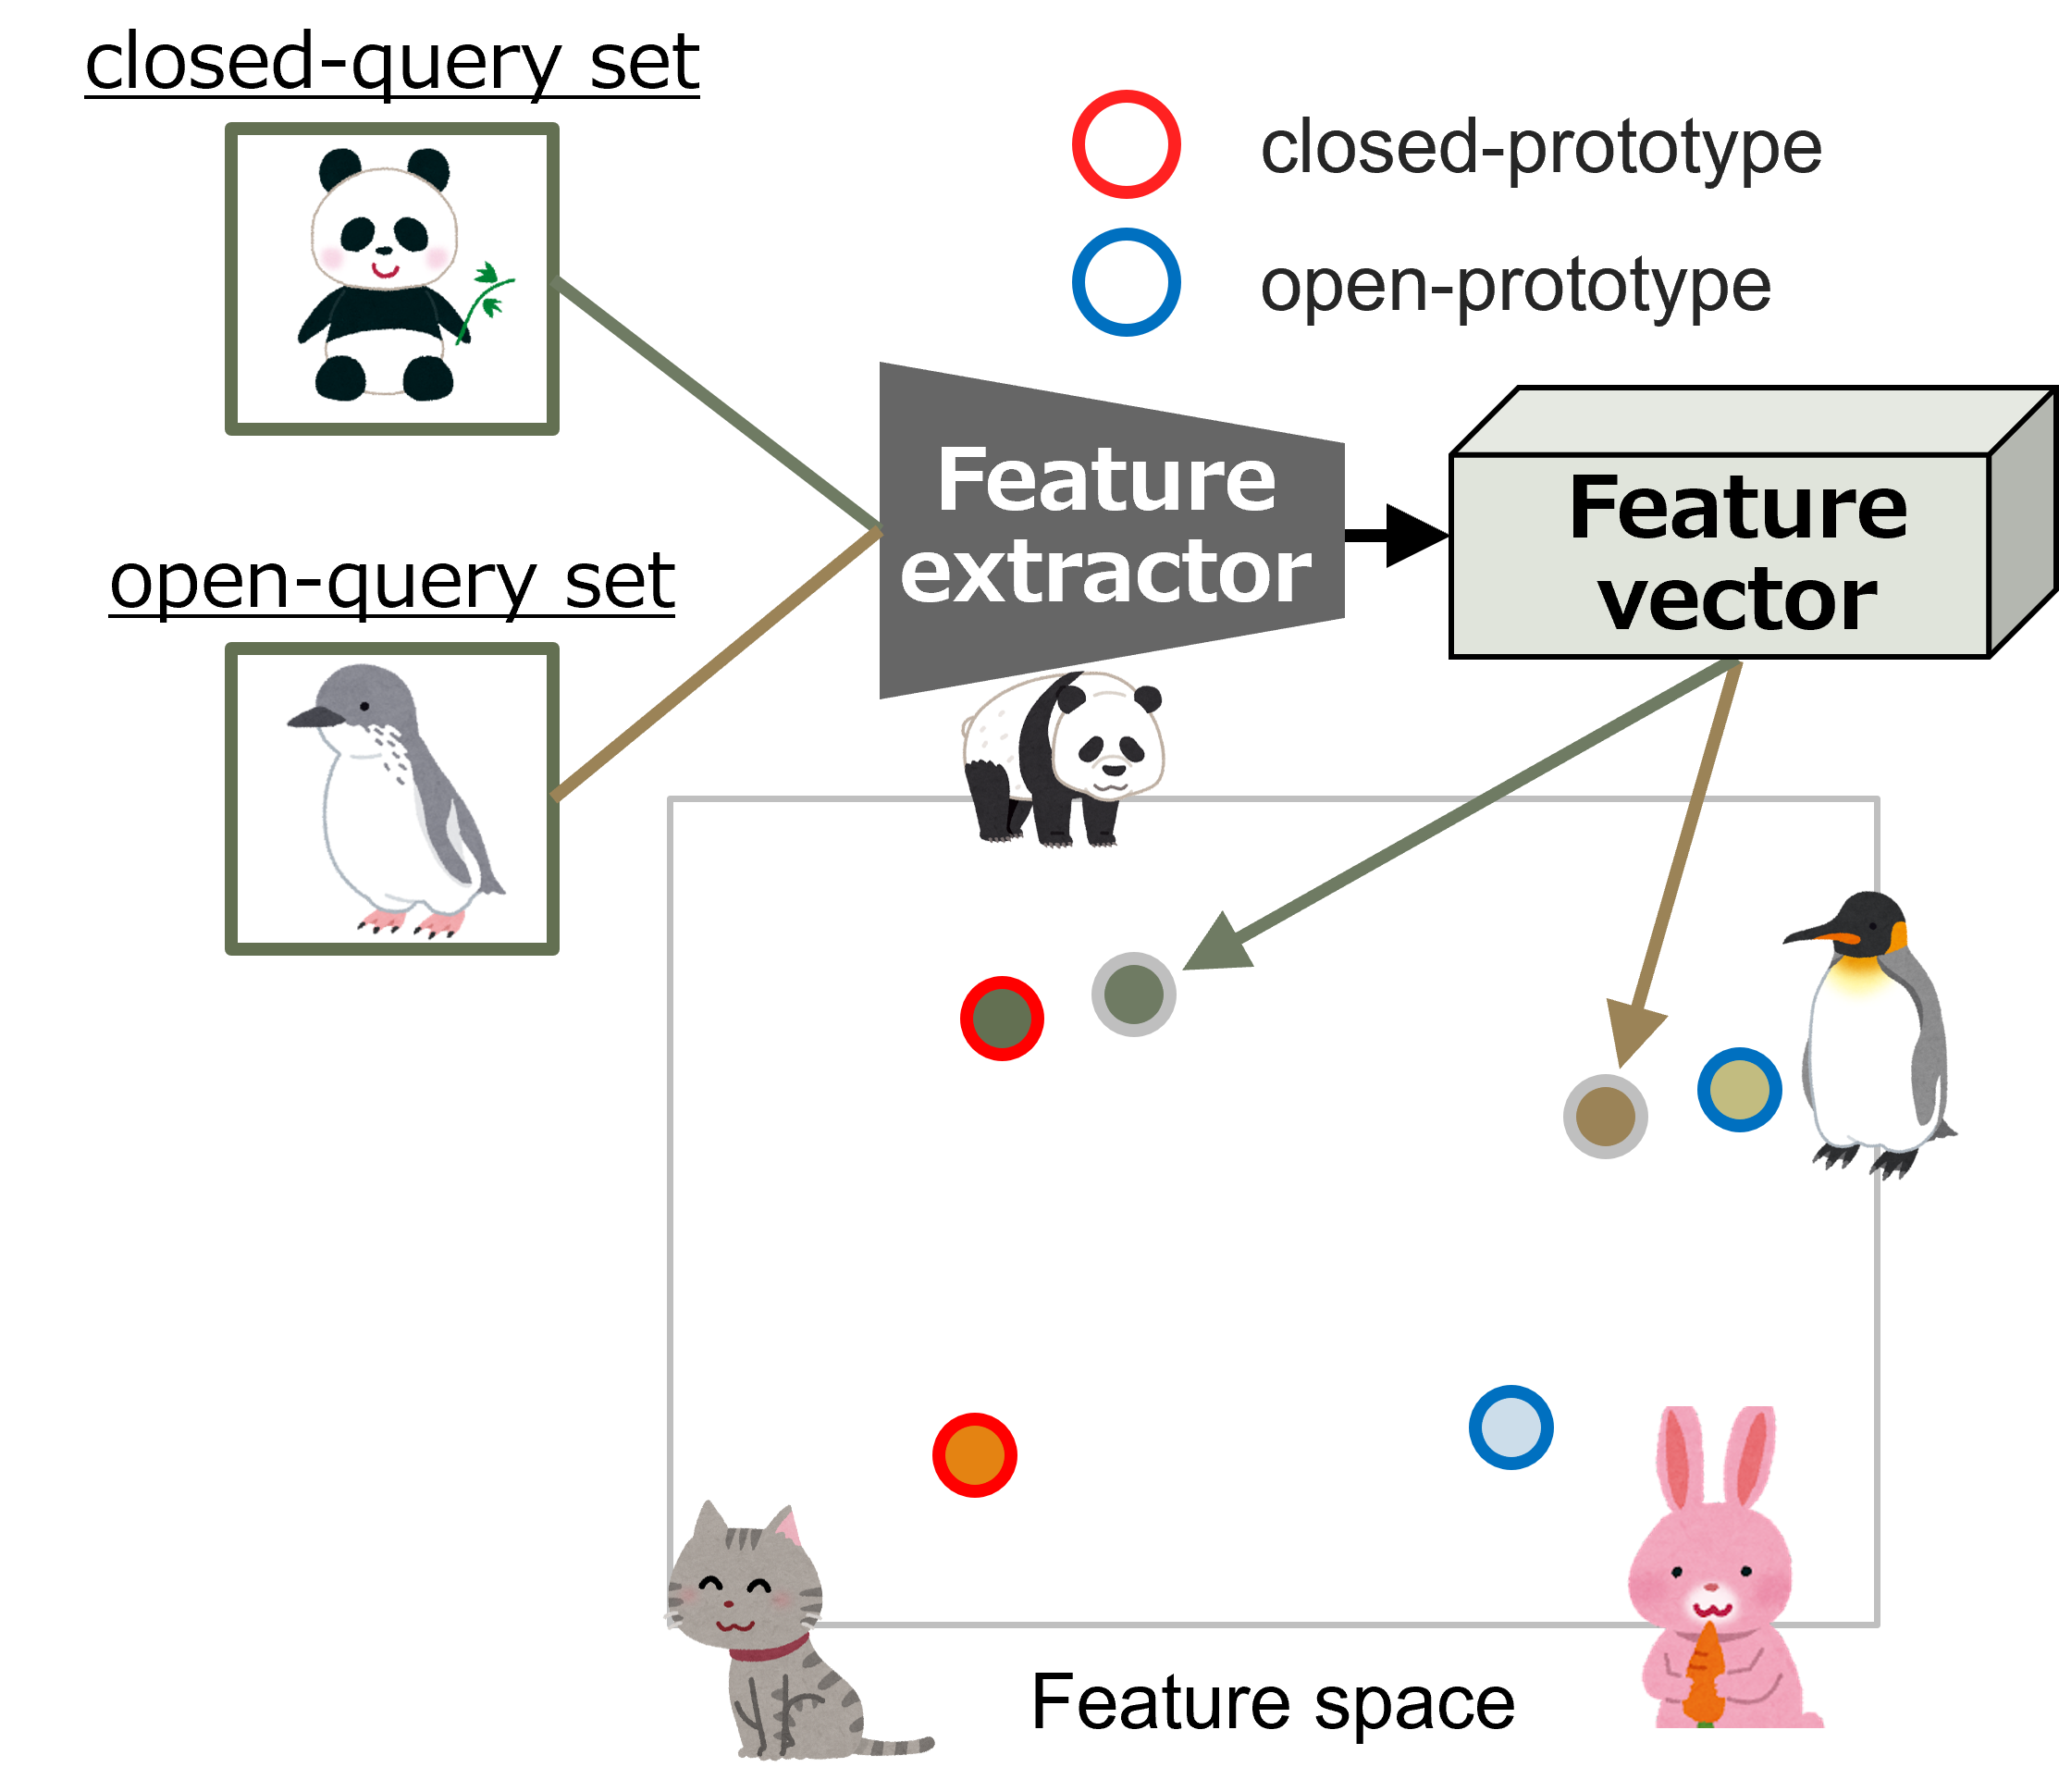
\includegraphics[width=0.8\linewidth, keepaspectratio]{image/open-prototype.png}
  \caption{クローズドプロトタイプとオープンプロトタイプを用いた評価方法}
  \label{fig:openprototype}
\end{figure}
% 
本評価方法においても,特徴抽出器に入力されたクエリセット中の画像は特徴空間上にプロットされ,距離が最も近いプロトタイプのクラスへと分類される.
分類精度は,このようにしてプロトタイプベースの分類が正しく行われた割合に基づき測定される.
ただし,\ref{sec:detect}節とは異なり,クエリデータの特徴点がオープンプロトタイプに近ければそのプロトタイプが属する未登録クラスに分類され,
クローズドプロトタイプに近ければそのプロトタイプが属する登録クラスに分類される.
この評価において,クローズドクエリデータのみの分類精度はClosed Accuracy,オープンクエリデータのみの分類精度はOpen Accuracy,
クローズドクエリデータとオープンクエリデータの分類精度を平均した精度はAll Accuracyとして表される.

本実験の評価設定としても5-Way,1-Shot問題を採用し,評価用データセットから各エピソードにおいて5つの登録クラスと5つの未登録クラスを選択した.
このうち,クローズドサポートセットとオープンサポートセットには1クラスにつき1枚の画像を選択し,クローズドクエリセットとオープンクエリセットには1クラスにつき15枚の画像を用いて評価を行った.

\subsection{実験結果及び考察}

表 \ref{tbl:exp4}に未登録の動物種の分類結果を示す.
% 
\begin{table*}[tbp]
  \centering
  \renewcommand{\arraystretch}{1.4}
  \caption{IFORにおけるk-means損失とBC損失のアブレーション結果}
  \label{tbl:exp4}
  % \footnotesize
  \small
  \setlength{\tabcolsep}{4pt} % 列幅のパディングをdefaltの6ptから4ptに変更
  \begin{tabular}{c||c|c||c|c|c|c} \hline
    学習フレームワーク                                        &    k-means   &      BC      & Closed Accuracy (\%) & Open Accuracy (\%) & All Accuracy (\%) &      AUROC     \\ \hline\hline
    \multirow{4}{*}{PEELER}                                &              &              &         38.3         &        37.8        &        38.1       & \textbf{49.7} \\ \cline{2-7}
                                                           & $\checkmark$ &              &         38.3         &        37.8        &        38.1       & \textbf{49.7} \\ \cline{2-7}
                                                           &              & $\checkmark$ &         38.3         &        37.8        &        38.1       & \textbf{49.7} \\ \cline{2-7}
                                                           & $\checkmark$ & $\checkmark$ &         39.0         &        38.3        &        38.7       &      49.6     \\ \hline
    \multirow{3}{*}{\shortstack[c]{PEELER\\(w/o 分類損失)}} & $\checkmark$ &              &         39.3         &    \textbf{39.2}   &        39.2       &      49.6     \\ \cline{2-7}
                                                           &              & $\checkmark$ &     \textbf{39.5}    &    \textbf{39.2}   &    \textbf{39.3}  &      49.6     \\ \cline{2-7}
                                                           & $\checkmark$ & $\checkmark$ &         39.3         &    \textbf{39.2}   &        39.2       &      49.6     \\ \hline
  \end{tabular}
\end{table*}
% 
本実験では,距離学習に基づくFSL損失とOSR損失に加え,分類損失を組み合わせた既存のPEELERフレームワークをベースラインとし,k-means損失,BC損失の有効性について検証を行った.
また,すべての実験において,PyTorch Image Models (timm)ライブラリ \cite{timm}によって提供される,
ImageNetで事前学習済みのViTモデル \texttt{deit\_tiny\_patch16\_224}を特徴抽出器として用いた.

結果より,既存手法のPEELERにk-means損失,または,BC損失を個別に組み合わせた場合,モデルの分類精度はベースラインとほぼ同等の性能であった.
一方,k-means損失とBC損失の両方をベースラインのPEELERに組み合わせることによって,ベースラインより高い性能を達成することが確認された.
次に,分類損失を用いないPEELERにk-means損失及びBC損失を組み合わせた結果を確認すると,k-means損失のみ,BC損失のみ,
k-means損失及びBC損失を組み合わせた場合のいずれにおいてもベースラインの精度より高くなることが確認された.
この結果は,IFORの5-Way,1-Shot問題において,分類損失を用いずにk-means損失やBC損失を単体で用いることの有効性を示している.

% 表 \ref{tbl:exp4}は,新規地域において1枚の画像のみを用いた学習という極めて厳しい条件下での評価結果である.
% ここから,前節の結果を載せるようにする
% しかし,実運用においては,新規地域で撮影された画像が徐々に蓄積されていくため,学習に利用可能な画像枚数 (サポートセット) は増加していく.
% Fig. 5では,評価時の学習画像数𝐾を変化させた場合の分類精度の推移を示した.

\ref{sec:detect}節の表 \ref{tbl:exp1}, \ref{tbl:exp2}及び \ref{tbl:exp3},本節の表 \ref{tbl:exp4}に示された結果は,新規地域においてサポートセットとしてわずか1枚の画像のみを使用するという,極めて厳しい条件下で評価されている.
しかし,システムの継続的な運用に伴い,サポートセットとして利用できる画像の数は自然に増加することが期待される.
このような実運用シナリオを考慮し,図 \ref{fig:k-shot}に示すように,評価時のショット数$K$が分類精度とAUROCに与える影響ついて検証を行った.
% 
\begin{figure}[tbp]
  \centering
  \begin{subfigure}[b]{0.45\linewidth}
    \centering
    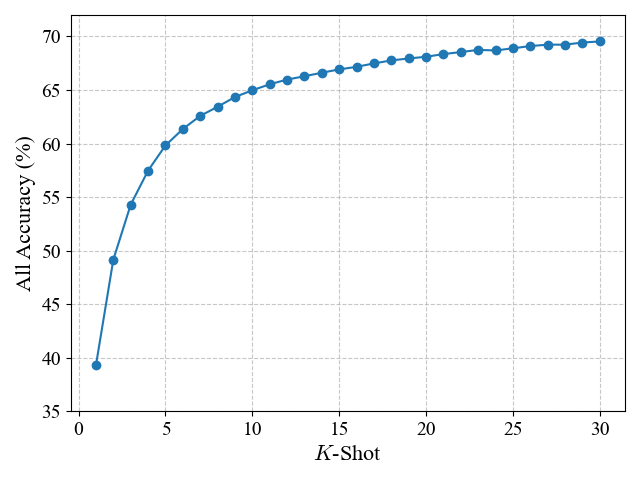
\includegraphics[height=0.9\linewidth, keepaspectratio]{image/sec2k-shotVSaccuracy.png}
    \caption{All Accuracyの推移}
    \label{fig:sec2Accuracy}
  \end{subfigure}
  \hfill
  \begin{subfigure}[b]{0.45\linewidth}
    \centering
    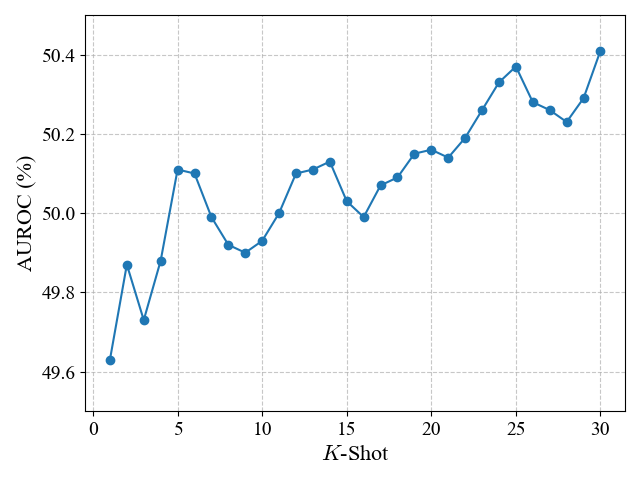
\includegraphics[height=0.9\linewidth, keepaspectratio]{image/sec2k-shotVSAUROC.png}
    \caption{AUROCの推移}
    \label{fig:sec2AUROC}
  \end{subfigure}
  \caption{評価時におけるサポートデータ数$K$が変化した際のAll AccuracyとAUROC}
  \label{fig:k-shot}
\end{figure}
% 
% 本評価では,特徴抽出器としてViT,転移学習手法としてImageNet,学習方法としてメタ学習を採用したモデルを使用した.
% 実験の結果,1クラスあたりの登録データの数を10枚,すなわち,10-shotとすることで,分類精度が75\%を超えることが確認された.
この評価では,特徴抽出器としてViT,転移学習手法としてImageNet,学習方法としてメタ学習,損失関数としてFSL損失,OSR損失,BC損失を採用したモデルを使用した.
実験の結果,図 \ref{fig:sec2Accuracy}に示すように,1クラスあたりのサポートデータを30枚,すなわち,30-Shotまで増加させることによって分類精度が約70\%に達することを確認した.
また,表 \ref{tbl:shot}に各カテゴリーにおける分類精度を示す.

% 表を修正する
\begin{table}[tbp]
  \centering
  \caption{サポートデータのShot数が変化した際の各カテゴリの分類精度}
  \label{tbl:shot}
  \begin{tabular}{c||c|c|c|c|c}
      \hline
      動物種        & 1-shot & 5-shot & 10-shot & 20-shot & 30-shot \\ \hline\hline
      bird         & 26.1   & 49.2   & 55.4    & 58.9    & 60.1    \\
      bobcat       & 36.7   & 55.7   & 59.8    & 61.6    & 64.7    \\
      cat          & 19.4   & 34.5   & 40.9    & 46.6    & 50.5    \\
      coyote       & 25.8   & 41.0   & 47.9    & 53.1    & 54.5    \\
      deer         & 55.4   & 81.9   & 86.1    & 88.0    & 88.1    \\
      dog          & 29.6   & 55.1   & 62.7    & 67.0    & 67.5    \\
      fox          & 34.3   & 47.7   & 54.3    & 58.9    & 60.7    \\
      opossum      & 47.2   & 70.1   & 75.5    & 79.1    & 80.6    \\
      rabbit       & 36.2   & 59.0   & 64.5    & 66.7    & 68.2    \\
      skunk        & 64.3   & 83.5   & 85.6    & 86.3    & 86.9    \\
      squirrel     & 56.7   & 79.1   & 80.9    & 81.6    & 81.9    \\ \hline\hline
      All Accuracy & 39.2   & 59.7   & 64.9    & 68.0    & 69.4    \\ \hline
  \end{tabular}
\end{table}

各実験結果の詳細な分析により,本研究における主要な課題として動物の姿勢による誤分類が明らかとなった.
特に,動物の背面のみが撮影された画像や複雑な姿勢をとる個体の画像など,出現頻度の低い姿勢パターンに対して分類精度の低下が観察された.
図 \ref{fig:animalback}は,このような姿勢の影響により誤分類された画像の具体的な事例を示している.
この課題に対する実用的な解決策としては,カメラトラップにより連続的に撮影された画像群をシーケンスデータとして扱うアプローチが有効である.
複数の連続画像における時間的文脈を考慮することにより,単一の画像からでは判断が困難な姿勢に対しても高精度な分類が期待できる.
この改善案は,モデルの頑健性及び実環境における適用可能性の向上に寄与しつつ,IFORフレームワークの本質的な利点を維持することが可能である.

\begin{figure}[tbp]
  \centering
  \begin{subfigure}[b]{0.45\linewidth}
    \centering
    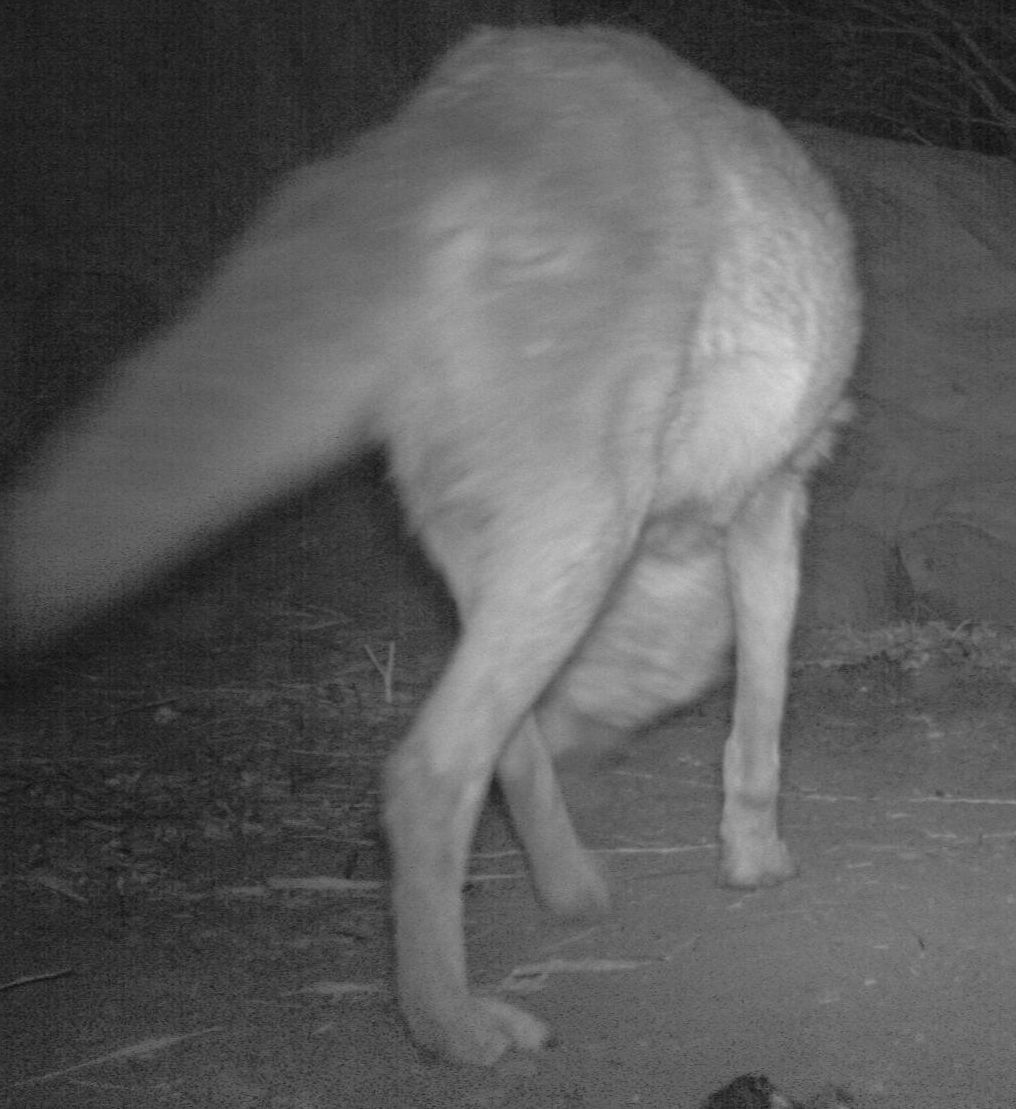
\includegraphics[height=0.9\linewidth, keepaspectratio]{image/coyote.png}
    \caption{coyoteの画像例}
    \label{fig:coyote}
  \end{subfigure}
  \hfill
  \begin{subfigure}[b]{0.45\linewidth}
    \centering
    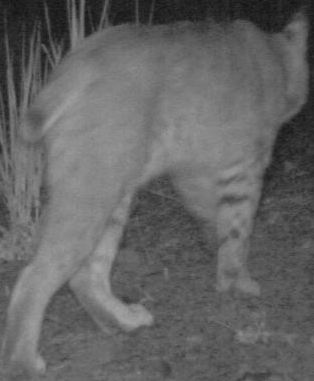
\includegraphics[height=0.9\linewidth, keepaspectratio]{image/bobcat.png}
    \caption{bobcatの画像例}
    \label{fig:bobcat}
  \end{subfigure}
  \caption{姿勢が原因で誤分類された画像例 (正解カテゴリ: coyote, 予測カテゴリ: bobcat)}
  \label{fig:animalback}
\end{figure}
% /01_draft/chapter5/chapter5_v2.tex

\chapter{結論}

本論文では,限られた赤外線画像を用いた効果的な野生動物モニタリングのための新たな概念として,Infrared Few-shot Open-set Recognition (IFOR)を提案した.
本研究では,最小限の赤外線画像データを用いて,モデルに登録された動物の分類と未登録の動物の識別を実現するIFORフレームワークを開発した.

包括的な分析により得られた主要な知見として,まず特徴抽出器について,ViTは赤外線画像の分類においてCNN(ResNet18)と比較して優れた性能を示し,分類精度が5.2\%向上した.
これは,ViTの大域的な注意機構が赤外線野生動物画像における特徴抽出において高い有効性を持つことを示唆している.
一方で,基盤モデルであるCLIPはViT-Baseと比較して有効性を示せなかった.
この結果を踏まえ,今後の研究課題として,テキストエンコーダやプロンプトを用いた学習フレームワークの検証が必要である.
これにより,IFORにおけるテキストと画像のペアを用いた対象学習の有効性を理論的かつ実験的に明らかにすることが可能となる.
転移学習については,ImageNetによる事前学習が,フラクタル画像ベースの事前学習及び事前学習なしの場合と比較して一貫して優れた性能を示した.
このことから,自然画像から学習した特徴抽出器が赤外線野生動物分類タスクに対して高い汎化性能を持つことを示している.
メタ学習に関しては,提案したメタ学習アプローチが従来の学習手法であるミニバッチ学習と比較して分類精度を11.1\%向上させ,未登録クラスに対する検出性能であるAUROCを7.7\%改善した.
この結果は,データ数が限られた条件下において,モデルを新規クラスに適応させる際のメタ学習の有効性を実証している.
未登録クラスの多クラス分類においては,k-means損失とBetween-Class損失の導入により既存のPEELERモデルと比較して,登録クラスと未登録クラスを含む全体の分類精度(All Accuracy)を改善した.
これらの実験により,クラスタリングに基づく損失関数が未登録クラスの多クラス分類に対して有効であることが実証された.

また,異なる地域から収集された学習用データセットと評価用データセットを用いることにより,ドメインシフト下におけるモデルの適応性に関する知見を得た.
さらに,学習に用いるサポートデータのShot数の増加がモデルの分類性能に及ぼす影響を検証し,Shot数を増やすことで分類精度が大幅に向上することを明らかにした.
これらの知見は,夜間環境という困難な条件下における野生動物モニタリング技術の進展に貢献するとともに,生態学の研究において直面する限られたデータ条件下でも適用可能な,
効率的かつ汎用性の高い機械学習モデルの開発に向けた基盤となる成果を提供している.

野生動物モニタリングの実用化に向けた今後の課題として,本研究で取り組んだ画像分類に加えて,物体検出手法の開発が挙げられる.
特に,少数の赤外線画像データという制約下においても,画像内の動物領域を高精度に検出可能な手法の開発が急務である.
また,将来の研究における有望な方向性として,IFORフレームワークの性能を潜在的に向上させる多段階転移学習アプローチが挙げられる.
具体的には,ImageNetのような大規模データセットにより事前学習されたモデルを基盤とし,Snapshot Serengetiのような大規模なカメラトラップ画像データセットを用いた中間的なファインチューニングを経て,
最終段階で,ターゲットタスクであるCCTやWCSのような小規模な赤外線画像データセットを用いたメタ学習を行うアプローチである.

% \chapter*{謝辞}
\tocack    % 目次に謝辞を追加
% /01_draft/chapter5/chapter5_v2.tex

\chapter*{謝辞}

本研究を進めるにあたり,全過程を通じて御助言,御指導を頂きました,滝本裕則教授に深謝の意を表します.

また,本研究及び本論文の執筆において,様々な面で御協力を頂きました,金川明弘名誉教授に感謝申し上げます.

そして,本研究の遂行にあたり日頃から御討論,御協力を頂いた数理情報メディア工学研究室の皆様に厚く御礼申し上げます.
特に,本研究の基盤となる研究を進められた伊藤嵐丸氏,岸本昌子氏に感謝の意を表します.
% 主な指導を受けた教員への言葉を最初に書く職位に気をつけること。
%本研究を進めるにあたり,終始様々な御助言,御指導を頂きました,滝本裕則准教授に深く感謝致します.

% 研究室の他の教員にお世話になったのであれば合わせて書く
%また,本研究及び本論文執筆の全過程を通じて,
%様々な面で御協力を頂きました,金川明弘教授に感謝致します.

% 研究室の学生への言葉も書くとよいだろう
%そして,本研究を通して日頃から御討論,
%御協力頂いた情報メディア工学研究室の皆様に心より御礼申し上げます.

% ほか,研究を進めるにあたりお世話になった方への感謝を示す


\tocpub    % 目次に研究業績を追加
% /01_draft/chapter5/chapter5_v2.tex

\chapter*{研究業績}

\subsection*{学術雑誌への掲載論文}
\begin{enumerate}
  \item 北山晃生, 岸孝樹, 古賀荘翠, 滝本裕則, 金川明弘, ``室内での見守り実現に向けた全方位画像に対する複数人物追跡,'' 日本福祉工学会誌, Vol.~26, No.~2, pp.~2-8(7ページ), 2024年11月.
  \item Koki Kishi, Ranmaru Ito, Sulfayanti Faharuddin Situju, Hironori Takimoto, and Akihiro Kanagawa, ``Animal Classification Considering Infrared Few-shot Open-set Recognition,'' \mbox{\textit{Cogent Engineering}}, (Accepted), 2025年1月.
\end{enumerate}

\subsection*{国際会議での研究発表}
\begin{enumerate}
  \item ◎Koki Kishi, Masako Kishimoto, Sulfayanti Faharuddin Situju, Hironori Takimoto and Akihiro Kanagawa, ``Few-Shot Learning for CNN-based Animal Classification in Camera Traps using an Infrared Camera,'' In \textit{Proceedings of the 10th IIAE International Conference on Intelligent Systems and Image Processing 2023 (ICISIP2023)}, pp.~11-17(7ページ), 2023年9月.
  \item ◎Koki Kishi, Ranmaru Ito, Sulfayanti Faharuddin Situju, Hironori Takimoto and Akihiro Kanagawa, ``Few-Shot Learning for Animal Classification in Camera Traps using an Infrared Camera,'' In \textit{Proceedings of the SICE Festival 2024 with Annual Conference (SICE FES 2024)}, WeBT7.7, pp.~420-423 (4ページ), 2024年8月.
\end{enumerate}

\subsection*{国内学会(全国レベル)での研究発表}
\begin{enumerate}
  \item ◎古賀荘翠, 北山晃生, 岸孝樹, 滝本裕則, 金川明弘, ``複数物体追跡におけるIDスイッチ抑制のためのMotion SORTの提案,'' 第28回 パターン計測シンポジウム, PM108\_04(4ページ), 2023年11月.
  \item ◎岸孝樹, 伊藤嵐丸, 植田諒大, Sulfayanti Faharuddin Situju, 滝本裕則, ``Infrared Few-shot Open-set Recognitionを考慮したクラスタリングとメタ学習による動物分類,'' 第29回 パターン計測シンポジウム, PM109\_02(8ページ), 2024年11月.
\end{enumerate}

\subsection*{国内学会(支部・県レベル)での研究発表}
\begin{enumerate}
  \item ◎岸孝樹, 伊藤嵐丸, 滝本裕則, 金川明弘, ``赤外線カメラトラップにおける動物分類のための少数データ学習,'' 第26回IEEE広島支部学生シンポジウム (IEEE HISS 26th) 論文集, TP-A-25, pp.~91-94(4ページ), 2024年11月.
\end{enumerate}

\subsection*{受賞}
\begin{enumerate}
  \item The 10th IIAE International Conference on Intelligent Systems and Image Processing 2023 Best Paper Award, 2023年9月(対象は上記の国際会議での研究発表(1)).
  \item 計測自動制御学会 計測部門 パターン計測部会 令和6年度優秀論文賞, 2024年11月(対象は上記の国内学会(全国レベル)での研究発表(2)).
  \item IEEE広島支部学生シンポジウム (HISS) 優秀研究賞, 2024年11月(対象は上記の国内学会(支部・県レベル)での研究発表(1)).
\end{enumerate}

\tocbib
\bibliographystyle{kishiIEEEtr}
\bibliography{references}

\end{document}
